%*************************************************************************
% A Classic Thesis Style
% An Homage to The Elements of Typographic Style
%
% Copyright (C) 2017 André Miede and Ivo Pletikosić
%
% If you like the style then I would appreciate a postcard. My address
% can be found in the file ClassicThesis.pdf. A collection of the
% postcards I received so far is available online at
% http://postcards.miede.de
%
% License:
% This program is free software; you can redistribute it and/or modify
% it under the terms of the GNU General Public License as published by
% the Free Software Foundation; either version 2 of the License, or
% (at your option) any later version.
%
% This program is distributed in the hope that it will be useful,
% but WITHOUT ANY WARRANTY; without even the implied warranty of
% MERCHANTABILITY or FITNESS FOR A PARTICULAR PURPOSE.  See the
% GNU General Public License for more details.
%
% You should have received a copy of the GNU General Public License
% along with this program; see the file COPYING.  If not, write to
% the Free Software Foundation, Inc., 59 Temple Place - Suite 330,
% Boston, MA 02111-1307, USA.
%
% PLEASE SEE ALSO THE AUTHORS' NOTE REGARDING THIS LICENSE
% IN THE DOCUMENTATION (ClassicThesis.pdf --> Chapter 1 / Chapter01.tex)
%*************************************************************************
\RequirePackage{silence} % :-\
    \WarningFilter{scrreprt}{Usage of package `titlesec'}
    %\WarningFilter{scrreprt}{Activating an ugly workaround}
    \WarningFilter{titlesec}{Non standard sectioning command detected}
\documentclass[ openright,titlepage,numbers=noenddot,headinclude,%twoside, %1headlines,% letterpaper a4paper
                footinclude=true,cleardoublepage=empty,abstractoff, % <--- obsolete, remove (todo)
                BCOR=5mm,paper=a4,fontsize=11pt,%11pt,a4paper,%
                ngerman,american,%lockflag%
                ]{scrreprt}

%*************************************************************************
% Note: Make all your adjustments in here
%*************************************************************************
% ****************************************************************************************************
% hdathesis-config.tex 
% Use it at the beginning of your thesis.tex, or as a LaTeX Preamble 
% in your thesis.{tex,lyx} with % ****************************************************************************************************
% hdathesis-config.tex 
% Use it at the beginning of your thesis.tex, or as a LaTeX Preamble 
% in your thesis.{tex,lyx} with % ****************************************************************************************************
% hdathesis-config.tex 
% Use it at the beginning of your thesis.tex, or as a LaTeX Preamble 
% in your thesis.{tex,lyx} with \input{hdathesis-config}
% ****************************************************************************************************

% ****************************************************************************************************
% 1. Personal data and user ad-hoc commands
% ****************************************************************************************************
\newcommand{\myTitle}{Characterisation of SiPM for LHCb SciFi Tracker 202X upgrade}
%\newcommand{\mySubtitle}{An Homage to The Elements of Typographic Style\xspace}
\newcommand{\myDegree}{Master of Science (B.Sc.)\xspace} 
%\newcommand{\myDegree}{Bachelor of Arts (B.A.)\xspace}
%\newcommand{\myDegree}{Master of Science (M.Sc.)\xspace}
%\newcommand{\myDegree}{Master of Arts (M.A.)\xspace}
\newcommand{\myName}{Matthieu Leydier\xspace}
%\newcommand{\myId}{081542\xspace}
\newcommand{\myProf}{Prof. Olivier Schneider\xspace}
\newcommand{\myOtherProf}{Prof. Dr. Martin Stiemerling\xspace}
\newcommand{\myFaculty}{Institute of Physics\xspace}
\newcommand{\myUni}{Swiss Federal Institute of Technology (EPFL) \xspace}
\newcommand{\myLocation}{Lausanne\xspace}
\newcommand{\myTime}{23. June 2023\xspace}
\newcommand{\myVersion}{version 4.4\xspace}

% ****************************************************************************************************
% 2. Is it a master thesis?
% ****************************************************************************************************
\PassOptionsToPackage{master}{hdahesis} % uncomment if this is a master thesis 

% ****************************************************************************************************
% 3. Does the thesis have a lock flag?
% ****************************************************************************************************
%\PassOptionsToPackage{lockflag}{hdathesis} % uncomment if this thesis has a lock flag 

% ****************************************************************************************************
% 4. Loading some handy packages
% ****************************************************************************************************
% ****************************************************************************************************
% Packages with options that might require adjustments
% ****************************************************************************************************

\PassOptionsToPackage{american}{babel}   % change this to your language(s)
% Spanish languages need extra options in order to work with this template
%\PassOptionsToPackage{spanish,es-lcroman}{babel}
\usepackage{babel}
\usepackage{subcaption}
%\usepackage[table,xcdraw]{xcolor}
\usepackage{booktabs}
\usepackage{natbib}
\usepackage{geometry}
\usepackage{pdflscape}

% ****************************************************************************************************

% ****************************************************************************************************
% 1. Personal data and user ad-hoc commands
% ****************************************************************************************************
\newcommand{\myTitle}{Characterisation of SiPM for LHCb SciFi Tracker 202X upgrade}
%\newcommand{\mySubtitle}{An Homage to The Elements of Typographic Style\xspace}
\newcommand{\myDegree}{Master of Science (B.Sc.)\xspace} 
%\newcommand{\myDegree}{Bachelor of Arts (B.A.)\xspace}
%\newcommand{\myDegree}{Master of Science (M.Sc.)\xspace}
%\newcommand{\myDegree}{Master of Arts (M.A.)\xspace}
\newcommand{\myName}{Matthieu Leydier\xspace}
%\newcommand{\myId}{081542\xspace}
\newcommand{\myProf}{Prof. Olivier Schneider\xspace}
\newcommand{\myOtherProf}{Prof. Dr. Martin Stiemerling\xspace}
\newcommand{\myFaculty}{Institute of Physics\xspace}
\newcommand{\myUni}{Swiss Federal Institute of Technology (EPFL) \xspace}
\newcommand{\myLocation}{Lausanne\xspace}
\newcommand{\myTime}{23. June 2023\xspace}
\newcommand{\myVersion}{version 4.4\xspace}

% ****************************************************************************************************
% 2. Is it a master thesis?
% ****************************************************************************************************
\PassOptionsToPackage{master}{hdahesis} % uncomment if this is a master thesis 

% ****************************************************************************************************
% 3. Does the thesis have a lock flag?
% ****************************************************************************************************
%\PassOptionsToPackage{lockflag}{hdathesis} % uncomment if this thesis has a lock flag 

% ****************************************************************************************************
% 4. Loading some handy packages
% ****************************************************************************************************
% ****************************************************************************************************
% Packages with options that might require adjustments
% ****************************************************************************************************

\PassOptionsToPackage{american}{babel}   % change this to your language(s)
% Spanish languages need extra options in order to work with this template
%\PassOptionsToPackage{spanish,es-lcroman}{babel}
\usepackage{babel}
\usepackage{subcaption}
%\usepackage[table,xcdraw]{xcolor}
\usepackage{booktabs}
\usepackage{natbib}
\usepackage{geometry}
\usepackage{pdflscape}

% ****************************************************************************************************

% ****************************************************************************************************
% 1. Personal data and user ad-hoc commands
% ****************************************************************************************************
\newcommand{\myTitle}{Characterisation of SiPM for LHCb SciFi Tracker 202X upgrade}
%\newcommand{\mySubtitle}{An Homage to The Elements of Typographic Style\xspace}
\newcommand{\myDegree}{Master of Science (B.Sc.)\xspace} 
%\newcommand{\myDegree}{Bachelor of Arts (B.A.)\xspace}
%\newcommand{\myDegree}{Master of Science (M.Sc.)\xspace}
%\newcommand{\myDegree}{Master of Arts (M.A.)\xspace}
\newcommand{\myName}{Matthieu Leydier\xspace}
%\newcommand{\myId}{081542\xspace}
\newcommand{\myProf}{Prof. Olivier Schneider\xspace}
\newcommand{\myOtherProf}{Prof. Dr. Martin Stiemerling\xspace}
\newcommand{\myFaculty}{Institute of Physics\xspace}
\newcommand{\myUni}{Swiss Federal Institute of Technology (EPFL) \xspace}
\newcommand{\myLocation}{Lausanne\xspace}
\newcommand{\myTime}{23. June 2023\xspace}
\newcommand{\myVersion}{version 4.4\xspace}

% ****************************************************************************************************
% 2. Is it a master thesis?
% ****************************************************************************************************
\PassOptionsToPackage{master}{hdahesis} % uncomment if this is a master thesis 

% ****************************************************************************************************
% 3. Does the thesis have a lock flag?
% ****************************************************************************************************
%\PassOptionsToPackage{lockflag}{hdathesis} % uncomment if this thesis has a lock flag 

% ****************************************************************************************************
% 4. Loading some handy packages
% ****************************************************************************************************
% ****************************************************************************************************
% Packages with options that might require adjustments
% ****************************************************************************************************

\PassOptionsToPackage{american}{babel}   % change this to your language(s)
% Spanish languages need extra options in order to work with this template
%\PassOptionsToPackage{spanish,es-lcroman}{babel}
\usepackage{babel}
\usepackage{subcaption}
%\usepackage[table,xcdraw]{xcolor}
\usepackage{booktabs}
\usepackage{natbib}
\usepackage{geometry}
\usepackage{pdflscape}

% ****************************************************************************************************
% classicthesis-config.tex
% formerly known as loadpackages.sty, classicthesis-ldpkg.sty, and classicthesis-preamble.sty
% Use it at the beginning of your ClassicThesis.tex, or as a LaTeX Preamble
% in your ClassicThesis.{tex,lyx} with % ****************************************************************************************************
% classicthesis-config.tex
% formerly known as loadpackages.sty, classicthesis-ldpkg.sty, and classicthesis-preamble.sty
% Use it at the beginning of your ClassicThesis.tex, or as a LaTeX Preamble
% in your ClassicThesis.{tex,lyx} with % ****************************************************************************************************
% classicthesis-config.tex
% formerly known as loadpackages.sty, classicthesis-ldpkg.sty, and classicthesis-preamble.sty
% Use it at the beginning of your ClassicThesis.tex, or as a LaTeX Preamble
% in your ClassicThesis.{tex,lyx} with \input{classicthesis-config}
% ****************************************************************************************************
% If you like the classicthesis, then I would appreciate a postcard.
% My address can be found in the file ClassicThesis.pdf. A collection
% of the postcards I received so far is available online at
% http://postcards.miede.de
% ****************************************************************************************************


% ****************************************************************************************************
% 0. Set the encoding of your files. UTF-8 is the only sensible encoding nowadays. If you can't read
% äöüßáéçèê∂åëæƒÏ€ then change the encoding setting in your editor, not the line below. If your editor
% does not support utf8 use another editor!
% ****************************************************************************************************
\PassOptionsToPackage{utf8}{inputenc}
  \usepackage{inputenc}

% ****************************************************************************************************
% 1. Configure classicthesis for your needs here, e.g., remove "drafting" below
% in order to deactivate the time-stamp on the pages
% (see ClassicThesis.pdf for more information):
% ****************************************************************************************************
\PassOptionsToPackage{
  drafting=false,   % print version information on the bottom of the pages
  tocaligned=false, % the left column of the toc will be aligned (no indentation)
  dottedtoc=true,   % page numbers in ToC flushed right
  parts=true,       % use part division
  eulerchapternumbers=true, % use AMS Euler for chapter font (otherwise Palatino)
  linedheaders=false,       % chaper headers will have line above and beneath
  floatperchapter=true,     % numbering per chapter for all floats (i.e., Figure 1.1)
  listings=true,    % load listings package and setup LoL
  subfig=true,      % setup for preloaded subfig package
  eulermath=false,  % use awesome Euler fonts for mathematical formulae (only with pdfLaTeX)
  beramono=true,    % toggle a nice monospaced font (w/ bold)
  minionpro=false   % setup for minion pro font; use minion pro small caps as well (only with pdfLaTeX)
}{classicthesis}


% ****************************************************************************************************
% 2. Personal data and user ad-hoc commands
% ****************************************************************************************************
%\newcommand{\myTitle}{A Classic Thesis Style\xspace}
%\newcommand{\mySubtitle}{An Homage to The Elements of Typographic Style\xspace}
%\newcommand{\myDegree}{Doktor-Ingenieur (Dr.-Ing.)\xspace}
%\newcommand{\myName}{André Miede\xspace}
%\newcommand{\myProf}{Put name here\xspace}
%\newcommand{\myOtherProf}{Put name here\xspace}
%\newcommand{\mySupervisor}{Put name here\xspace}
%\newcommand{\myFaculty}{Put data here\xspace}
%\newcommand{\myDepartment}{Put data here\xspace}
%\newcommand{\myUni}{Put data here\xspace}
%\newcommand{\myLocation}{Saarbrücken\xspace}
%\newcommand{\myTime}{October 2017\xspace}
%\newcommand{\myVersion}{version 4.4}

% ********************************************************************
% Setup, finetuning, and useful commands
% ********************************************************************
\newcounter{dummy} % necessary for correct hyperlinks (to index, bib, etc.)
\newlength{\abcd} % for ab..z string length calculation
\providecommand{\mLyX}{L\kern-.1667em\lower.25em\hbox{Y}\kern-.125emX\@}
\newcommand{\ie}{i.\,e.}
\newcommand{\Ie}{I.\,e.}
\newcommand{\eg}{e.\,g.}
\newcommand{\Eg}{E.\,g.}
% ****************************************************************************************************


% ****************************************************************************************************
% 3. Loading some handy packages
% ****************************************************************************************************
% ********************************************************************
% Packages with options that might require adjustments
% ********************************************************************
%\PassOptionsToPackage{ngerman,american}{babel}   % change this to your language(s), main language last
% Spanish languages need extra options in order to work with this template
%\PassOptionsToPackage{spanish,es-lcroman}{babel}
\usepackage{babel}

\usepackage{csquotes}


\PassOptionsToPackage{%
  backend=biber,bibencoding=utf8, %instead of bibtex
  %backend=bibtex8,bibencoding=ascii,%
  language=auto,%
  %style=numeric-comp,%
  style=numeric,%alphabetic
  %style=authoryear-comp, % Author 1999, 2010
  %bibstyle=authoryear,dashed=false, % dashed: substitute rep. author with ---
  sorting=none%nyt, % name, year, title
  maxbibnames=10, % default: 3, et al.
  backref=true,%
  natbib=true % natbib compatibility mode (\citep and \citet still work)
}{biblatex}
  %\usepackage{biblatex}

\PassOptionsToPackage{fleqn}{amsmath}       % math environments and more by the AMS
  \usepackage{amsmath}

\PassOptionsToPackage{doublespacing}{hdathesis}  % options: abbrev exam big wiwi english master
  \usepackage{hdathesis}

% ********************************************************************
% General useful packages
% ********************************************************************
\PassOptionsToPackage{T1}{fontenc} % T2A for cyrillics
  \usepackage{fontenc}
\usepackage{textcomp} % fix warning with missing font shapes
\usepackage{scrhack} % fix warnings when using KOMA with listings package
\usepackage{xspace} % to get the spacing after macros right
\usepackage{mparhack} % get marginpar right
%\usepackage{fixltx2e} % fixes some LaTeX stuff --> since 2015 in the LaTeX kernel (see below)
% \usepackage[latest]{latexrelease} % emulate newer kernel version if older is detected
\PassOptionsToPackage{printonlyused,smaller}{acronym}
  \usepackage{acronym} % nice macros for handling all acronyms in the thesis
  %\renewcommand{\bflabel}[1]{{#1}\hfill} % fix the list of acronyms --> no longer working
  %\renewcommand*{\acsfont}[1]{\textsc{#1}}
  %\renewcommand*{\aclabelfont}[1]{\acsfont{#1}}
  %\def\bflabel#1{{#1\hfill}}
  \def\bflabel#1{{\acsfont{#1}\hfill}}
  \def\aclabelfont#1{\acsfont{#1}}
% ****************************************************************************************************
%\usepackage{pgfplots} % External TikZ/PGF support (thanks to Andreas Nautsch)
%\usetikzlibrary{external}
%\tikzexternalize[mode=list and make, prefix=ext-tikz/]
% ****************************************************************************************************


% ****************************************************************************************************
% 4. Setup floats: tables, (sub)figures, and captions
% ****************************************************************************************************
\usepackage{tabularx} % better tables
  \setlength{\extrarowheight}{3pt} % increase table row height
\newcommand{\tableheadline}[1]{\multicolumn{1}{c}{\spacedlowsmallcaps{#1}}}
\newcommand{\myfloatalign}{\centering} % to be used with each float for alignment
\usepackage{caption}
% Thanks to cgnieder and Claus Lahiri
% http://tex.stackexchange.com/questions/69349/spacedlowsmallcaps-in-caption-label
% [REMOVED DUE TO OTHER PROBLEMS, SEE ISSUE #82]
%\DeclareCaptionLabelFormat{smallcaps}{\bothIfFirst{#1}{~}\MakeTextLowercase{\textsc{#2}}}
%\captionsetup{font=small,labelformat=smallcaps} % format=hang,
\captionsetup{font=small} % format=hang,
\usepackage{subfig}
% ****************************************************************************************************


% ****************************************************************************************************
% 5. Setup code listings
% ****************************************************************************************************
\usepackage{listings}
%\lstset{emph={trueIndex,root},emphstyle=\color{BlueViolet}}%\underbar} % for special keywords
\lstset{language=[LaTeX]Tex,%C++,
  morekeywords={PassOptionsToPackage,selectlanguage},
  keywordstyle=\color{RoyalBlue},%\bfseries,
  basicstyle=\small\ttfamily,
  %identifierstyle=\color{NavyBlue},
  commentstyle=\color{Green}\ttfamily,
  stringstyle=\rmfamily,
  numbers=none,%left,%
  numberstyle=\scriptsize,%\tiny
  stepnumber=5,
  numbersep=8pt,
  showstringspaces=false,
  breaklines=true,
  %frameround=ftff,
  %frame=single,
  belowcaptionskip=.75\baselineskip
  %frame=L
}
% ****************************************************************************************************
% 6. PDFLaTeX, hyperreferences, and citation backreferences
% ****************************************************************************************************
% ********************************************************************
% Using PDFLaTeX
% ********************************************************************
\PassOptionsToPackage{hyperfootnotes=false,pdfpagelabels}{hyperref}
  \usepackage{hyperref}  % backref linktocpage 
%pagebackref
%\ifpdf
%\pdfcompresslevel=9
%\pdfadjustspacing=1
%\fi
%\PassOptionsToPackage{pdftex}{graphicx} %%%IVO: driver will be chosen automatically
  \usepackage{graphicx}
  \usepackage{url}


% ********************************************************************
% Hyperreferences
% ********************************************************************
\hypersetup{%
  %draft, % hyperref's draft mode, for printing see below
  colorlinks=true, linktocpage=true, pdfstartpage=3, pdfstartview=FitV,%
  % uncomment the following line if you want to have black links (e.g., for printing)
  %colorlinks=false, linktocpage=false, pdfstartpage=3, pdfstartview=FitV, pdfborder={0 0 0},%
  breaklinks=true, pdfpagemode=UseNone, pageanchor=true, pdfpagemode=UseOutlines,%
  plainpages=false, bookmarksnumbered, bookmarksopen=true, bookmarksopenlevel=1,%
  hypertexnames=true, pdfhighlight=/O,%nesting=true,%frenchlinks,%
  urlcolor=webbrown, linkcolor=RoyalBlue, citecolor=webgreen, %pagecolor=RoyalBlue,%
  %urlcolor=Black, linkcolor=Black, citecolor=Black, %pagecolor=Black,%
  pdftitle={\myTitle},%
  pdfauthor={\textcopyright\ \myName, \myUni, \myFaculty},%
  pdfsubject={},%
  pdfkeywords={},%
  pdfcreator={pdfLaTeX},%
  pdfproducer={LaTeX with hyperref and classicthesis}%
}

% ********************************************************************
% Setup autoreferences
% ********************************************************************
% There are some issues regarding autorefnames
% http://www.ureader.de/msg/136221647.aspx
% http://www.tex.ac.uk/cgi-bin/texfaq2html?label=latexwords
% you have to redefine the makros for the
% language you use, e.g., american, ngerman
% (as chosen when loading babel/AtBeginDocument)
% ********************************************************************
\makeatletter
\@ifpackageloaded{babel}%
  {%
    \addto\extrasamerican{%
      \renewcommand*{\figureautorefname}{Figure}%
      \renewcommand*{\tableautorefname}{Table}%
      \renewcommand*{\partautorefname}{Part}%
      \renewcommand*{\chapterautorefname}{Chapter}%
      \renewcommand*{\sectionautorefname}{Section}%
      \renewcommand*{\subsectionautorefname}{Section}%
      \renewcommand*{\subsubsectionautorefname}{Section}%
    }%
    \addto\extrasngerman{%
      \renewcommand*{\paragraphautorefname}{Absatz}%
      \renewcommand*{\subparagraphautorefname}{Unterabsatz}%
      \renewcommand*{\footnoteautorefname}{Fu\"snote}%
      \renewcommand*{\FancyVerbLineautorefname}{Zeile}%
      \renewcommand*{\theoremautorefname}{Theorem}%
      \renewcommand*{\appendixautorefname}{Anhang}%
      \renewcommand*{\equationautorefname}{Gleichung}%
      \renewcommand*{\itemautorefname}{Punkt}%
    }%
      % Fix to getting autorefs for subfigures right (thanks to Belinda Vogt for changing the definition)
      \providecommand{\subfigureautorefname}{\figureautorefname}%
    }{\relax}
\makeatother


% ****************************************************************************************************
% 7. Last calls before the bar closes
% ****************************************************************************************************
% ********************************************************************
% Development Stuff
% ********************************************************************
\listfiles
%\PassOptionsToPackage{l2tabu,orthodox,abort}{nag}
%  \usepackage{nag}
%\PassOptionsToPackage{warning, all}{onlyamsmath}
%  \usepackage{onlyamsmath}

% ********************************************************************
% Last, but not least...
% ********************************************************************
\usepackage{classicthesis}
% 
\usepackage{subcaption}
\usepackage{subfigure}
% 
% 8. Further adjustments (experimental)
% 
% Changing the text area
% 
%\areaset[current]{312pt}{761pt} % 686 (factor 2.2) + 33 head + 42 head \the\footskip
%\setlength{\marginparwidth}{7em}%
%\setlength{\marginparsep}{2em}%

% 
% Using different fonts
% ********************************************************************
%\usepackage[oldstylenums]{kpfonts} % oldstyle notextcomp
%\usepackage[osf]{libertine}
%\usepackage[light,condensed,math]{iwona}
%\renewcommand{\sfdefault}{iwona}
%\usepackage{lmodern} % <-- no osf support :-(
%\usepackage{cfr-lm} %
%\usepackage[urw-garamond]{mathdesign} <-- no osf support :-(
%\usepackage[default,osfigures]{opensans} % scale=0.95
%\usepackage[sfdefault]{FiraSans}
% ********************************************************************
% \usepackage[largesc,osf]{newpxtext}
% Used to fix these:
% https://bitbucket.org/amiede/classicthesis/issues/139/italics-in-pallatino-capitals-chapter
% https://bitbucket.org/amiede/classicthesis/issues/45/problema-testatine-su-classicthesis-style
% ********************************************************************
%\linespread{1.05} % a bit more for Palatino
% ****************************************************************************************************
\usepackage{subcaption}
%\usepackage[table,xcdraw]{xcolor}
\usepackage{booktabs}
\usepackage{siunitx}
\usepackage{natbib}
\usepackage{wrapfig}
\usepackage{geometry}
\usepackage{pdflscape}

% ****************************************************************************************************
% If you like the classicthesis, then I would appreciate a postcard.
% My address can be found in the file ClassicThesis.pdf. A collection
% of the postcards I received so far is available online at
% http://postcards.miede.de
% ****************************************************************************************************


% ****************************************************************************************************
% 0. Set the encoding of your files. UTF-8 is the only sensible encoding nowadays. If you can't read
% äöüßáéçèê∂åëæƒÏ€ then change the encoding setting in your editor, not the line below. If your editor
% does not support utf8 use another editor!
% ****************************************************************************************************
\PassOptionsToPackage{utf8}{inputenc}
  \usepackage{inputenc}

% ****************************************************************************************************
% 1. Configure classicthesis for your needs here, e.g., remove "drafting" below
% in order to deactivate the time-stamp on the pages
% (see ClassicThesis.pdf for more information):
% ****************************************************************************************************
\PassOptionsToPackage{
  drafting=false,   % print version information on the bottom of the pages
  tocaligned=false, % the left column of the toc will be aligned (no indentation)
  dottedtoc=true,   % page numbers in ToC flushed right
  parts=true,       % use part division
  eulerchapternumbers=true, % use AMS Euler for chapter font (otherwise Palatino)
  linedheaders=false,       % chaper headers will have line above and beneath
  floatperchapter=true,     % numbering per chapter for all floats (i.e., Figure 1.1)
  listings=true,    % load listings package and setup LoL
  subfig=true,      % setup for preloaded subfig package
  eulermath=false,  % use awesome Euler fonts for mathematical formulae (only with pdfLaTeX)
  beramono=true,    % toggle a nice monospaced font (w/ bold)
  minionpro=false   % setup for minion pro font; use minion pro small caps as well (only with pdfLaTeX)
}{classicthesis}


% ****************************************************************************************************
% 2. Personal data and user ad-hoc commands
% ****************************************************************************************************
%\newcommand{\myTitle}{A Classic Thesis Style\xspace}
%\newcommand{\mySubtitle}{An Homage to The Elements of Typographic Style\xspace}
%\newcommand{\myDegree}{Doktor-Ingenieur (Dr.-Ing.)\xspace}
%\newcommand{\myName}{André Miede\xspace}
%\newcommand{\myProf}{Put name here\xspace}
%\newcommand{\myOtherProf}{Put name here\xspace}
%\newcommand{\mySupervisor}{Put name here\xspace}
%\newcommand{\myFaculty}{Put data here\xspace}
%\newcommand{\myDepartment}{Put data here\xspace}
%\newcommand{\myUni}{Put data here\xspace}
%\newcommand{\myLocation}{Saarbrücken\xspace}
%\newcommand{\myTime}{October 2017\xspace}
%\newcommand{\myVersion}{version 4.4}

% ********************************************************************
% Setup, finetuning, and useful commands
% ********************************************************************
\newcounter{dummy} % necessary for correct hyperlinks (to index, bib, etc.)
\newlength{\abcd} % for ab..z string length calculation
\providecommand{\mLyX}{L\kern-.1667em\lower.25em\hbox{Y}\kern-.125emX\@}
\newcommand{\ie}{i.\,e.}
\newcommand{\Ie}{I.\,e.}
\newcommand{\eg}{e.\,g.}
\newcommand{\Eg}{E.\,g.}
% ****************************************************************************************************


% ****************************************************************************************************
% 3. Loading some handy packages
% ****************************************************************************************************
% ********************************************************************
% Packages with options that might require adjustments
% ********************************************************************
%\PassOptionsToPackage{ngerman,american}{babel}   % change this to your language(s), main language last
% Spanish languages need extra options in order to work with this template
%\PassOptionsToPackage{spanish,es-lcroman}{babel}
\usepackage{babel}

\usepackage{csquotes}


\PassOptionsToPackage{%
  backend=biber,bibencoding=utf8, %instead of bibtex
  %backend=bibtex8,bibencoding=ascii,%
  language=auto,%
  %style=numeric-comp,%
  style=numeric,%alphabetic
  %style=authoryear-comp, % Author 1999, 2010
  %bibstyle=authoryear,dashed=false, % dashed: substitute rep. author with ---
  sorting=none%nyt, % name, year, title
  maxbibnames=10, % default: 3, et al.
  backref=true,%
  natbib=true % natbib compatibility mode (\citep and \citet still work)
}{biblatex}
  %\usepackage{biblatex}

\PassOptionsToPackage{fleqn}{amsmath}       % math environments and more by the AMS
  \usepackage{amsmath}

\PassOptionsToPackage{doublespacing}{hdathesis}  % options: abbrev exam big wiwi english master
  \usepackage{hdathesis}

% ********************************************************************
% General useful packages
% ********************************************************************
\PassOptionsToPackage{T1}{fontenc} % T2A for cyrillics
  \usepackage{fontenc}
\usepackage{textcomp} % fix warning with missing font shapes
\usepackage{scrhack} % fix warnings when using KOMA with listings package
\usepackage{xspace} % to get the spacing after macros right
\usepackage{mparhack} % get marginpar right
%\usepackage{fixltx2e} % fixes some LaTeX stuff --> since 2015 in the LaTeX kernel (see below)
% \usepackage[latest]{latexrelease} % emulate newer kernel version if older is detected
\PassOptionsToPackage{printonlyused,smaller}{acronym}
  \usepackage{acronym} % nice macros for handling all acronyms in the thesis
  %\renewcommand{\bflabel}[1]{{#1}\hfill} % fix the list of acronyms --> no longer working
  %\renewcommand*{\acsfont}[1]{\textsc{#1}}
  %\renewcommand*{\aclabelfont}[1]{\acsfont{#1}}
  %\def\bflabel#1{{#1\hfill}}
  \def\bflabel#1{{\acsfont{#1}\hfill}}
  \def\aclabelfont#1{\acsfont{#1}}
% ****************************************************************************************************
%\usepackage{pgfplots} % External TikZ/PGF support (thanks to Andreas Nautsch)
%\usetikzlibrary{external}
%\tikzexternalize[mode=list and make, prefix=ext-tikz/]
% ****************************************************************************************************


% ****************************************************************************************************
% 4. Setup floats: tables, (sub)figures, and captions
% ****************************************************************************************************
\usepackage{tabularx} % better tables
  \setlength{\extrarowheight}{3pt} % increase table row height
\newcommand{\tableheadline}[1]{\multicolumn{1}{c}{\spacedlowsmallcaps{#1}}}
\newcommand{\myfloatalign}{\centering} % to be used with each float for alignment
\usepackage{caption}
% Thanks to cgnieder and Claus Lahiri
% http://tex.stackexchange.com/questions/69349/spacedlowsmallcaps-in-caption-label
% [REMOVED DUE TO OTHER PROBLEMS, SEE ISSUE #82]
%\DeclareCaptionLabelFormat{smallcaps}{\bothIfFirst{#1}{~}\MakeTextLowercase{\textsc{#2}}}
%\captionsetup{font=small,labelformat=smallcaps} % format=hang,
\captionsetup{font=small} % format=hang,
\usepackage{subfig}
% ****************************************************************************************************


% ****************************************************************************************************
% 5. Setup code listings
% ****************************************************************************************************
\usepackage{listings}
%\lstset{emph={trueIndex,root},emphstyle=\color{BlueViolet}}%\underbar} % for special keywords
\lstset{language=[LaTeX]Tex,%C++,
  morekeywords={PassOptionsToPackage,selectlanguage},
  keywordstyle=\color{RoyalBlue},%\bfseries,
  basicstyle=\small\ttfamily,
  %identifierstyle=\color{NavyBlue},
  commentstyle=\color{Green}\ttfamily,
  stringstyle=\rmfamily,
  numbers=none,%left,%
  numberstyle=\scriptsize,%\tiny
  stepnumber=5,
  numbersep=8pt,
  showstringspaces=false,
  breaklines=true,
  %frameround=ftff,
  %frame=single,
  belowcaptionskip=.75\baselineskip
  %frame=L
}
% ****************************************************************************************************
% 6. PDFLaTeX, hyperreferences, and citation backreferences
% ****************************************************************************************************
% ********************************************************************
% Using PDFLaTeX
% ********************************************************************
\PassOptionsToPackage{hyperfootnotes=false,pdfpagelabels}{hyperref}
  \usepackage{hyperref}  % backref linktocpage 
%pagebackref
%\ifpdf
%\pdfcompresslevel=9
%\pdfadjustspacing=1
%\fi
%\PassOptionsToPackage{pdftex}{graphicx} %%%IVO: driver will be chosen automatically
  \usepackage{graphicx}
  \usepackage{url}


% ********************************************************************
% Hyperreferences
% ********************************************************************
\hypersetup{%
  %draft, % hyperref's draft mode, for printing see below
  colorlinks=true, linktocpage=true, pdfstartpage=3, pdfstartview=FitV,%
  % uncomment the following line if you want to have black links (e.g., for printing)
  %colorlinks=false, linktocpage=false, pdfstartpage=3, pdfstartview=FitV, pdfborder={0 0 0},%
  breaklinks=true, pdfpagemode=UseNone, pageanchor=true, pdfpagemode=UseOutlines,%
  plainpages=false, bookmarksnumbered, bookmarksopen=true, bookmarksopenlevel=1,%
  hypertexnames=true, pdfhighlight=/O,%nesting=true,%frenchlinks,%
  urlcolor=webbrown, linkcolor=RoyalBlue, citecolor=webgreen, %pagecolor=RoyalBlue,%
  %urlcolor=Black, linkcolor=Black, citecolor=Black, %pagecolor=Black,%
  pdftitle={\myTitle},%
  pdfauthor={\textcopyright\ \myName, \myUni, \myFaculty},%
  pdfsubject={},%
  pdfkeywords={},%
  pdfcreator={pdfLaTeX},%
  pdfproducer={LaTeX with hyperref and classicthesis}%
}

% ********************************************************************
% Setup autoreferences
% ********************************************************************
% There are some issues regarding autorefnames
% http://www.ureader.de/msg/136221647.aspx
% http://www.tex.ac.uk/cgi-bin/texfaq2html?label=latexwords
% you have to redefine the makros for the
% language you use, e.g., american, ngerman
% (as chosen when loading babel/AtBeginDocument)
% ********************************************************************
\makeatletter
\@ifpackageloaded{babel}%
  {%
    \addto\extrasamerican{%
      \renewcommand*{\figureautorefname}{Figure}%
      \renewcommand*{\tableautorefname}{Table}%
      \renewcommand*{\partautorefname}{Part}%
      \renewcommand*{\chapterautorefname}{Chapter}%
      \renewcommand*{\sectionautorefname}{Section}%
      \renewcommand*{\subsectionautorefname}{Section}%
      \renewcommand*{\subsubsectionautorefname}{Section}%
    }%
    \addto\extrasngerman{%
      \renewcommand*{\paragraphautorefname}{Absatz}%
      \renewcommand*{\subparagraphautorefname}{Unterabsatz}%
      \renewcommand*{\footnoteautorefname}{Fu\"snote}%
      \renewcommand*{\FancyVerbLineautorefname}{Zeile}%
      \renewcommand*{\theoremautorefname}{Theorem}%
      \renewcommand*{\appendixautorefname}{Anhang}%
      \renewcommand*{\equationautorefname}{Gleichung}%
      \renewcommand*{\itemautorefname}{Punkt}%
    }%
      % Fix to getting autorefs for subfigures right (thanks to Belinda Vogt for changing the definition)
      \providecommand{\subfigureautorefname}{\figureautorefname}%
    }{\relax}
\makeatother


% ****************************************************************************************************
% 7. Last calls before the bar closes
% ****************************************************************************************************
% ********************************************************************
% Development Stuff
% ********************************************************************
\listfiles
%\PassOptionsToPackage{l2tabu,orthodox,abort}{nag}
%  \usepackage{nag}
%\PassOptionsToPackage{warning, all}{onlyamsmath}
%  \usepackage{onlyamsmath}

% ********************************************************************
% Last, but not least...
% ********************************************************************
\usepackage{classicthesis}
% 
\usepackage{subcaption}
\usepackage{subfigure}
% 
% 8. Further adjustments (experimental)
% 
% Changing the text area
% 
%\areaset[current]{312pt}{761pt} % 686 (factor 2.2) + 33 head + 42 head \the\footskip
%\setlength{\marginparwidth}{7em}%
%\setlength{\marginparsep}{2em}%

% 
% Using different fonts
% ********************************************************************
%\usepackage[oldstylenums]{kpfonts} % oldstyle notextcomp
%\usepackage[osf]{libertine}
%\usepackage[light,condensed,math]{iwona}
%\renewcommand{\sfdefault}{iwona}
%\usepackage{lmodern} % <-- no osf support :-(
%\usepackage{cfr-lm} %
%\usepackage[urw-garamond]{mathdesign} <-- no osf support :-(
%\usepackage[default,osfigures]{opensans} % scale=0.95
%\usepackage[sfdefault]{FiraSans}
% ********************************************************************
% \usepackage[largesc,osf]{newpxtext}
% Used to fix these:
% https://bitbucket.org/amiede/classicthesis/issues/139/italics-in-pallatino-capitals-chapter
% https://bitbucket.org/amiede/classicthesis/issues/45/problema-testatine-su-classicthesis-style
% ********************************************************************
%\linespread{1.05} % a bit more for Palatino
% ****************************************************************************************************
\usepackage{subcaption}
%\usepackage[table,xcdraw]{xcolor}
\usepackage{booktabs}
\usepackage{siunitx}
\usepackage{natbib}
\usepackage{wrapfig}
\usepackage{geometry}
\usepackage{pdflscape}

% ****************************************************************************************************
% If you like the classicthesis, then I would appreciate a postcard.
% My address can be found in the file ClassicThesis.pdf. A collection
% of the postcards I received so far is available online at
% http://postcards.miede.de
% ****************************************************************************************************


% ****************************************************************************************************
% 0. Set the encoding of your files. UTF-8 is the only sensible encoding nowadays. If you can't read
% äöüßáéçèê∂åëæƒÏ€ then change the encoding setting in your editor, not the line below. If your editor
% does not support utf8 use another editor!
% ****************************************************************************************************
\PassOptionsToPackage{utf8}{inputenc}
  \usepackage{inputenc}

% ****************************************************************************************************
% 1. Configure classicthesis for your needs here, e.g., remove "drafting" below
% in order to deactivate the time-stamp on the pages
% (see ClassicThesis.pdf for more information):
% ****************************************************************************************************
\PassOptionsToPackage{
  drafting=false,   % print version information on the bottom of the pages
  tocaligned=false, % the left column of the toc will be aligned (no indentation)
  dottedtoc=true,   % page numbers in ToC flushed right
  parts=true,       % use part division
  eulerchapternumbers=true, % use AMS Euler for chapter font (otherwise Palatino)
  linedheaders=false,       % chaper headers will have line above and beneath
  floatperchapter=true,     % numbering per chapter for all floats (i.e., Figure 1.1)
  listings=true,    % load listings package and setup LoL
  subfig=true,      % setup for preloaded subfig package
  eulermath=false,  % use awesome Euler fonts for mathematical formulae (only with pdfLaTeX)
  beramono=true,    % toggle a nice monospaced font (w/ bold)
  minionpro=false   % setup for minion pro font; use minion pro small caps as well (only with pdfLaTeX)
}{classicthesis}


% ****************************************************************************************************
% 2. Personal data and user ad-hoc commands
% ****************************************************************************************************
%\newcommand{\myTitle}{A Classic Thesis Style\xspace}
%\newcommand{\mySubtitle}{An Homage to The Elements of Typographic Style\xspace}
%\newcommand{\myDegree}{Doktor-Ingenieur (Dr.-Ing.)\xspace}
%\newcommand{\myName}{André Miede\xspace}
%\newcommand{\myProf}{Put name here\xspace}
%\newcommand{\myOtherProf}{Put name here\xspace}
%\newcommand{\mySupervisor}{Put name here\xspace}
%\newcommand{\myFaculty}{Put data here\xspace}
%\newcommand{\myDepartment}{Put data here\xspace}
%\newcommand{\myUni}{Put data here\xspace}
%\newcommand{\myLocation}{Saarbrücken\xspace}
%\newcommand{\myTime}{October 2017\xspace}
%\newcommand{\myVersion}{version 4.4}

% ********************************************************************
% Setup, finetuning, and useful commands
% ********************************************************************
\newcounter{dummy} % necessary for correct hyperlinks (to index, bib, etc.)
\newlength{\abcd} % for ab..z string length calculation
\providecommand{\mLyX}{L\kern-.1667em\lower.25em\hbox{Y}\kern-.125emX\@}
\newcommand{\ie}{i.\,e.}
\newcommand{\Ie}{I.\,e.}
\newcommand{\eg}{e.\,g.}
\newcommand{\Eg}{E.\,g.}
% ****************************************************************************************************


% ****************************************************************************************************
% 3. Loading some handy packages
% ****************************************************************************************************
% ********************************************************************
% Packages with options that might require adjustments
% ********************************************************************
%\PassOptionsToPackage{ngerman,american}{babel}   % change this to your language(s), main language last
% Spanish languages need extra options in order to work with this template
%\PassOptionsToPackage{spanish,es-lcroman}{babel}
\usepackage{babel}

\usepackage{csquotes}


\PassOptionsToPackage{%
  backend=biber,bibencoding=utf8, %instead of bibtex
  %backend=bibtex8,bibencoding=ascii,%
  language=auto,%
  %style=numeric-comp,%
  style=numeric,%alphabetic
  %style=authoryear-comp, % Author 1999, 2010
  %bibstyle=authoryear,dashed=false, % dashed: substitute rep. author with ---
  sorting=none%nyt, % name, year, title
  maxbibnames=10, % default: 3, et al.
  backref=true,%
  natbib=true % natbib compatibility mode (\citep and \citet still work)
}{biblatex}
  %\usepackage{biblatex}

\PassOptionsToPackage{fleqn}{amsmath}       % math environments and more by the AMS
  \usepackage{amsmath}

\PassOptionsToPackage{doublespacing}{hdathesis}  % options: abbrev exam big wiwi english master
  \usepackage{hdathesis}

% ********************************************************************
% General useful packages
% ********************************************************************
\PassOptionsToPackage{T1}{fontenc} % T2A for cyrillics
  \usepackage{fontenc}
\usepackage{textcomp} % fix warning with missing font shapes
\usepackage{scrhack} % fix warnings when using KOMA with listings package
\usepackage{xspace} % to get the spacing after macros right
\usepackage{mparhack} % get marginpar right
%\usepackage{fixltx2e} % fixes some LaTeX stuff --> since 2015 in the LaTeX kernel (see below)
% \usepackage[latest]{latexrelease} % emulate newer kernel version if older is detected
\PassOptionsToPackage{printonlyused,smaller}{acronym}
  \usepackage{acronym} % nice macros for handling all acronyms in the thesis
  %\renewcommand{\bflabel}[1]{{#1}\hfill} % fix the list of acronyms --> no longer working
  %\renewcommand*{\acsfont}[1]{\textsc{#1}}
  %\renewcommand*{\aclabelfont}[1]{\acsfont{#1}}
  %\def\bflabel#1{{#1\hfill}}
  \def\bflabel#1{{\acsfont{#1}\hfill}}
  \def\aclabelfont#1{\acsfont{#1}}
% ****************************************************************************************************
%\usepackage{pgfplots} % External TikZ/PGF support (thanks to Andreas Nautsch)
%\usetikzlibrary{external}
%\tikzexternalize[mode=list and make, prefix=ext-tikz/]
% ****************************************************************************************************


% ****************************************************************************************************
% 4. Setup floats: tables, (sub)figures, and captions
% ****************************************************************************************************
\usepackage{tabularx} % better tables
  \setlength{\extrarowheight}{3pt} % increase table row height
\newcommand{\tableheadline}[1]{\multicolumn{1}{c}{\spacedlowsmallcaps{#1}}}
\newcommand{\myfloatalign}{\centering} % to be used with each float for alignment
\usepackage{caption}
% Thanks to cgnieder and Claus Lahiri
% http://tex.stackexchange.com/questions/69349/spacedlowsmallcaps-in-caption-label
% [REMOVED DUE TO OTHER PROBLEMS, SEE ISSUE #82]
%\DeclareCaptionLabelFormat{smallcaps}{\bothIfFirst{#1}{~}\MakeTextLowercase{\textsc{#2}}}
%\captionsetup{font=small,labelformat=smallcaps} % format=hang,
\captionsetup{font=small} % format=hang,
\usepackage{subfig}
% ****************************************************************************************************


% ****************************************************************************************************
% 5. Setup code listings
% ****************************************************************************************************
\usepackage{listings}
%\lstset{emph={trueIndex,root},emphstyle=\color{BlueViolet}}%\underbar} % for special keywords
\lstset{language=[LaTeX]Tex,%C++,
  morekeywords={PassOptionsToPackage,selectlanguage},
  keywordstyle=\color{RoyalBlue},%\bfseries,
  basicstyle=\small\ttfamily,
  %identifierstyle=\color{NavyBlue},
  commentstyle=\color{Green}\ttfamily,
  stringstyle=\rmfamily,
  numbers=none,%left,%
  numberstyle=\scriptsize,%\tiny
  stepnumber=5,
  numbersep=8pt,
  showstringspaces=false,
  breaklines=true,
  %frameround=ftff,
  %frame=single,
  belowcaptionskip=.75\baselineskip
  %frame=L
}
% ****************************************************************************************************
% 6. PDFLaTeX, hyperreferences, and citation backreferences
% ****************************************************************************************************
% ********************************************************************
% Using PDFLaTeX
% ********************************************************************
\PassOptionsToPackage{hyperfootnotes=false,pdfpagelabels}{hyperref}
  \usepackage{hyperref}  % backref linktocpage 
%pagebackref
%\ifpdf
%\pdfcompresslevel=9
%\pdfadjustspacing=1
%\fi
%\PassOptionsToPackage{pdftex}{graphicx} %%%IVO: driver will be chosen automatically
  \usepackage{graphicx}
  \usepackage{url}


% ********************************************************************
% Hyperreferences
% ********************************************************************
\hypersetup{%
  %draft, % hyperref's draft mode, for printing see below
  colorlinks=true, linktocpage=true, pdfstartpage=3, pdfstartview=FitV,%
  % uncomment the following line if you want to have black links (e.g., for printing)
  %colorlinks=false, linktocpage=false, pdfstartpage=3, pdfstartview=FitV, pdfborder={0 0 0},%
  breaklinks=true, pdfpagemode=UseNone, pageanchor=true, pdfpagemode=UseOutlines,%
  plainpages=false, bookmarksnumbered, bookmarksopen=true, bookmarksopenlevel=1,%
  hypertexnames=true, pdfhighlight=/O,%nesting=true,%frenchlinks,%
  urlcolor=webbrown, linkcolor=RoyalBlue, citecolor=webgreen, %pagecolor=RoyalBlue,%
  %urlcolor=Black, linkcolor=Black, citecolor=Black, %pagecolor=Black,%
  pdftitle={\myTitle},%
  pdfauthor={\textcopyright\ \myName, \myUni, \myFaculty},%
  pdfsubject={},%
  pdfkeywords={},%
  pdfcreator={pdfLaTeX},%
  pdfproducer={LaTeX with hyperref and classicthesis}%
}

% ********************************************************************
% Setup autoreferences
% ********************************************************************
% There are some issues regarding autorefnames
% http://www.ureader.de/msg/136221647.aspx
% http://www.tex.ac.uk/cgi-bin/texfaq2html?label=latexwords
% you have to redefine the makros for the
% language you use, e.g., american, ngerman
% (as chosen when loading babel/AtBeginDocument)
% ********************************************************************
\makeatletter
\@ifpackageloaded{babel}%
  {%
    \addto\extrasamerican{%
      \renewcommand*{\figureautorefname}{Figure}%
      \renewcommand*{\tableautorefname}{Table}%
      \renewcommand*{\partautorefname}{Part}%
      \renewcommand*{\chapterautorefname}{Chapter}%
      \renewcommand*{\sectionautorefname}{Section}%
      \renewcommand*{\subsectionautorefname}{Section}%
      \renewcommand*{\subsubsectionautorefname}{Section}%
    }%
    \addto\extrasngerman{%
      \renewcommand*{\paragraphautorefname}{Absatz}%
      \renewcommand*{\subparagraphautorefname}{Unterabsatz}%
      \renewcommand*{\footnoteautorefname}{Fu\"snote}%
      \renewcommand*{\FancyVerbLineautorefname}{Zeile}%
      \renewcommand*{\theoremautorefname}{Theorem}%
      \renewcommand*{\appendixautorefname}{Anhang}%
      \renewcommand*{\equationautorefname}{Gleichung}%
      \renewcommand*{\itemautorefname}{Punkt}%
    }%
      % Fix to getting autorefs for subfigures right (thanks to Belinda Vogt for changing the definition)
      \providecommand{\subfigureautorefname}{\figureautorefname}%
    }{\relax}
\makeatother


% ****************************************************************************************************
% 7. Last calls before the bar closes
% ****************************************************************************************************
% ********************************************************************
% Development Stuff
% ********************************************************************
\listfiles
%\PassOptionsToPackage{l2tabu,orthodox,abort}{nag}
%  \usepackage{nag}
%\PassOptionsToPackage{warning, all}{onlyamsmath}
%  \usepackage{onlyamsmath}

% ********************************************************************
% Last, but not least...
% ********************************************************************
\usepackage{classicthesis}
% 
\usepackage{subcaption}
\usepackage{subfigure}
% 
% 8. Further adjustments (experimental)
% 
% Changing the text area
% 
%\areaset[current]{312pt}{761pt} % 686 (factor 2.2) + 33 head + 42 head \the\footskip
%\setlength{\marginparwidth}{7em}%
%\setlength{\marginparsep}{2em}%

% 
% Using different fonts
% ********************************************************************
%\usepackage[oldstylenums]{kpfonts} % oldstyle notextcomp
%\usepackage[osf]{libertine}
%\usepackage[light,condensed,math]{iwona}
%\renewcommand{\sfdefault}{iwona}
%\usepackage{lmodern} % <-- no osf support :-(
%\usepackage{cfr-lm} %
%\usepackage[urw-garamond]{mathdesign} <-- no osf support :-(
%\usepackage[default,osfigures]{opensans} % scale=0.95
%\usepackage[sfdefault]{FiraSans}
% ********************************************************************
% \usepackage[largesc,osf]{newpxtext}
% Used to fix these:
% https://bitbucket.org/amiede/classicthesis/issues/139/italics-in-pallatino-capitals-chapter
% https://bitbucket.org/amiede/classicthesis/issues/45/problema-testatine-su-classicthesis-style
% ********************************************************************
%\linespread{1.05} % a bit more for Palatino
% ****************************************************************************************************
\usepackage{subcaption}
%\usepackage[table,xcdraw]{xcolor}
\usepackage{booktabs}
\usepackage{siunitx}
\usepackage{natbib}
\usepackage{wrapfig}
\usepackage{geometry}
\usepackage{pdflscape}


%*************************************************************************
% Bibliographies
%*************************************************************************
%\usepackage[backend=biber,style=authoryear]{biblatex}
%\addbibresource{references.bib}

%\addbibresource{bibliography.bib}

%*************************************************************************
% Hyphenation
%*************************************************************************
%\hyphenation{put special hyphenation here}

%*************************************************************************
% GO!GO!GO! MOVE IT!
%*************************************************************************
\begin{document}

\frenchspacing
\raggedbottom
\selectlanguage{american} % ngerman, american
%\renewcommand*{\bibname}{new name}
%\setbibpreamble{}
\pagenumbering{roman}
\pagestyle{plain}
%*************************************************************************
% Frontmatter
%*************************************************************************
%*******************************************************
% Titlepage
%*******************************************************
%%%
%%% title page (german)
%%%
\thispagestyle{empty}
\pdfbookmark[0]{Titelblatt}{title}
\begin{titlepage}

  % If printed on two sides, center the title page
  \condTWOSIDE{\changetext{}{19mm}{}{19mm}{}}

  \vspace{1cm}
  \begin{center}
    
\includegraphics[width=5.7cm]{gfx/logoep.png} \\ 
  \end{center}

  \begin{center}
    \vspace{0.1cm}
    \huge \textbf{Swiss Federal Institute of Technology (EPFL)}\\
    \vspace{0.4cm}
    \LARGE --~Institute of Physics~--
  \end{center}

  \vfill
  \vfill

  \begin{center}
    \LARGE \textbf{Characterisation of SiPMs for the LHCb SciFi Tracker upgrade}
  \end{center} 

  \vfill
  \vfill

  \begin{center}
    \Large Master thesis for the award of \\
    \vspace{0.3cm}
    \Large Master of Science MSc in Physics
  \end{center}

  \vfill

  \begin{center}
    \Large Submitted by\\
    \vspace{0.3cm}
    \Large \textbf{Matthieu Leydier}\\
    \vspace{0.3cm}
    \normalsize SCIPER Number: 288509
  \end{center}

  \vfill
  \vfill

  \begin{center}
    \begin{tabular}{lll}
      Referent    & : & Prof. Olivier Schneider and Guido Haefeli \\
      Supervisor & : & Ettore Zaffaroni  
    \end{tabular}
  \end{center} 

  % If printed on two sides, center the title page
  \condTWOSIDE{\changetext{}{-19mm}{}{-19mm}{}}

\end{titlepage}

\thispagestyle{empty}

\hfill

\vfill

\noindent Matthieu Leydier: \textit{Characterisation of SiPMs for the LHCb SciFi Tracker upgrade}, \ifdef{\mySubtitle}{\mySubtitle,}{} %\myDegree,
\textcopyright\ \myTime

%\bigskip
%
%\noindent\spacedlowsmallcaps{Supervisors}: \\
%\myProf \\
%\myOtherProf \\
%\mySupervisor
%
%\medskip
%
%\noindent\spacedlowsmallcaps{Location}: \\
%\myLocation
%
%\medskip
%
%\noindent\spacedlowsmallcaps{Time Frame}: \\
%\myTime

%\cleardoublepage\include{frontbackmatter/Dedication}
%\cleardoublepage\include{frontbackmatter/Foreword}
%\cleardoublepage%*******************************************************
% Declaration
%*******************************************************
\refstepcounter{dummy}
\pdfbookmark[0]{Declaration}{declaration}
\chapter*{\condENGLISH{Declaration}{Acknowledgement}}
\thispagestyle{empty}
To my parents and family for their unconditional support throughout the years 
\medskip

\noindent
yesyes
\medskip

\noindent
Die Zeichnungen oder Abbildungen in dieser Arbeit sind von mir selbst erstellt worden oder mit einem entsprechenden Quellennachweis versehen.
\medskip

\noindent
Diese Arbeit ist in gleicher oder ähnlicher Form noch bei keiner anderen Prüfungsbehörde eingereicht worden. 
\bigskip

\noindent\textit{Lausanne, \myTime}

\smallskip

\begin{flushright}
    \begin{tabular}{m{5cm}}
        \\ \hline
        \centering Matthieu Leydier \\
    \end{tabular}
\end{flushright}

\condLOCK{\cleardoublepage\include{frontbackmatter/BlockingNotice}}
\cleardoublepage%*******************************************************
% Abstract in English
%*******************************************************
\pdfbookmark[0]{Abstract}{Abstract}


\begin{otherlanguage}{american}
	\chapter*{Abstract}
The work presented in the thesis has been conducted as part of the research and development (R\&D) efforts for the \ac{SciFi} tracker of the LHCb experiment at CERN.  More precisely, new SiPMs are being considered for future upgrades. This report presents a comprehensive characterisation of the \ac{SiPM} array developed at the \ac{FBK} with the near ultraviolet high density (NUV-HD) technology. \\
\\
As a reference and tool of comparison, the actual SiPM used in the SciFi tracker from Hamamatsu, the H2017 is characterised with methods developed in \cite{Girard2018CharacterisationDistributions} that are used as a baseline for the characterisation of the FBK SiPM. The quenching resistors $R_Q$, breakdown voltage $V_{bd}$, correlated noise, gain, and \ac{PDE} are measured. \\
\\
The results from the characterisation showed a higher operation range for the FBK compared to the Hamamatsu.
The FBK detectors showed a correlated noise value significantly lower than the H2017, with values from $3.8\%$ to $5.8\%$ at $\Delta V = 12$ V compared to $9.5\%$ at $\Delta V = 4.4$ V for the H2017. \\

The PDE of the FBK detectors reaches a maximum around \SI{410}{\nano m} of $29\%$, $52\%$, $57\%$ for the \SI{16}{\micro m} , \SI{31}{\micro m} and \SI{42}{\micro m} respectively, at $\Delta V = 12$ V. The Hamamatsu H2017 has at $\lambda \approx 470$ nm a peak PDE of $40\%$ at $\Delta V = 4.4$ V. Adding an epoxy layer on the FBK \SI{31}{\micro m} cancelled the oscillations one the PDE value and reduced it by $10\%$ of the \SI{31}{\micro m} bare die with a peak efficiency of $46\%$ at $\Delta V=12$ V.
The low correlated noise value for the FBK detectors allow to reach a higher PDE than the Hamamatsu.\\

This work has continued the development of methods to characterise the FBK NUV-HD detectors. \\
\\

Keywords: \textit{Silicon Photo Multiplier SiPM, Characterisation, FBK NUV-HD, Quenching resistor, Breakdown Voltage, Correlated Noise, Gain, Photo-Detection Efficiency.}

\end{otherlanguage}


%\cleardoublepage%*******************************************************
% Abstract in English
%*******************************************************
\pdfbookmark[0]{Abstract}{Abstract}


\begin{otherlanguage}{american}
	\chapter*{Abstract}
The work presented in the thesis has been conducted as part of the research and development (R\&D) efforts for the \ac{SciFi} tracker of the LHCb experiment at CERN.  More precisely, new SiPMs are being considered for future upgrades. This report presents a comprehensive characterisation of the \ac{SiPM} array developed at the \ac{FBK} with the near ultraviolet high density (NUV-HD) technology. \\
\\
As a reference and tool of comparison, the actual SiPM used in the SciFi tracker from Hamamatsu, the H2017 is characterised with methods developed in \cite{Girard2018CharacterisationDistributions} that are used as a baseline for the characterisation of the FBK SiPM. The quenching resistors $R_Q$, breakdown voltage $V_{bd}$, correlated noise, gain, and \ac{PDE} are measured. \\
\\
The results from the characterisation showed a higher operation range for the FBK compared to the Hamamatsu.
The FBK detectors showed a correlated noise value significantly lower than the H2017, with values from $3.8\%$ to $5.8\%$ at $\Delta V = 12$ V compared to $9.5\%$ at $\Delta V = 4.4$ V for the H2017. \\

The PDE of the FBK detectors reaches a maximum around \SI{410}{\nano m} of $29\%$, $52\%$, $57\%$ for the \SI{16}{\micro m} , \SI{31}{\micro m} and \SI{42}{\micro m} respectively, at $\Delta V = 12$ V. The Hamamatsu H2017 has at $\lambda \approx 470$ nm a peak PDE of $40\%$ at $\Delta V = 4.4$ V. Adding an epoxy layer on the FBK \SI{31}{\micro m} cancelled the oscillations one the PDE value and reduced it by $10\%$ of the \SI{31}{\micro m} bare die with a peak efficiency of $46\%$ at $\Delta V=12$ V.
The low correlated noise value for the FBK detectors allow to reach a higher PDE than the Hamamatsu.\\

This work has continued the development of methods to characterise the FBK NUV-HD detectors. \\
\\

Keywords: \textit{Silicon Photo Multiplier SiPM, Characterisation, FBK NUV-HD, Quenching resistor, Breakdown Voltage, Correlated Noise, Gain, Photo-Detection Efficiency.}

\end{otherlanguage}


%\cleardoublepage\include{frontbackmatter/Publications}
\cleardoublepage%*******************************************************
% Acknowledgments
%*******************************************************
\pdfbookmark[0]{Acknowledgments}{acknowledgments}

%\begin{flushright}{\slshape
%Ouuuuhouuuu \\
%On s'habitue toujours à tout
%} \\ \medskip
%    --- Angele - Profite% \citep{Angele}
%\end{flushright}

\bigskip

\begingroup
\let\clearpage\relax
\let\cleardoublepage\relax
\let\cleardoublepage\relax
\chapter*{Acknowledgments}
I am grateful to my thesis supervisor, Ettore Zaffaroni, and my referees, Prof. Olivier Schneider and Guido Haefeli, who guided me throughout the entire project. Their counsel and insights have been precious in completing this work.

The LPHE has been an important place during this master program, and I express my gratitude to every member of the laboratory for their participation in the life of this group.

I would like to thank my parents for their unconditional support throughout the years. My friends and family have always been there when needed, and I am more than grateful to them.


\endgroup




\cleardoublepage\include{frontbackmatter/Contents}
%\cleardoublepage\include{frontbackmatter/Listings}
\cleardoublepage%*******************************************************
% Acronyms
%*******************************************************
\automark[section]{chapter}
\renewcommand{\chaptermark}[1]{\markboth{\spacedlowsmallcaps{#1}}{\spacedlowsmallcaps{#1}}}
\renewcommand{\sectionmark}[1]{\markright{\thesection\enspace\spacedlowsmallcaps{#1}}}
\refstepcounter{dummy}
\pdfbookmark[0]{Abk\"{u}rzungsverzeichnis}{abkuerzungsverzeichnis}
\markboth{\spacedlowsmallcaps{Abk\"{u}rzungsverzeichnis}}{\spacedlowsmallcaps{Abk\"{u}rzungsverzeichnis}}
\chapter*{List of acronyms}

% Insert your acronyms here
\begin{acronym}[UML]
  %\acro{DRY}{Don't Repeat Yourself}
  %\acro{API}{Application Programming Interface}
  %\acro{UML}{Unified Modeling Language}
  \acro{FBK}{Fundation Bruno Kessler}
  \acro{SiPM}{Silicon Photo-Multiplier}
  \acro{SiPMs}{Silicon Photo-Multipliers}
  \acro{APD}{Avalanche Photo-Diode}
  \acro{APDs}{Avalanche Photo-Diodes}
  \acro{FB}{Forward Bias Region}
  \acro{RB}{Reverse Bias Region}
  \acro{SPAD}{Single Photon Avalanche Diode}
  \acro{SPADs}{Single Photon Avalanche Diodes}
  \acro{G-APD}{Geiger Mode Avalanche Photo-Diode}
  \acro{FF}{Fill Factor}
  \acro{PE}{Photo-Electron}
  \acro{DiXT}{Direct Cross Talk}
  \acro{DeXT}{Delayed Cross Talk}
  \acro{AP}{After Pulse}
  \acro{PDE}{Photo Detection Efficiency}
  \acro{ECAL}{Electromagetic Calorimeter}
  \acro{SciFi}{Scintillating Fibers}
  \acro{PCB}{Printed Circuit Board}
  \acro{NUV-HD}{Near Ultraviolet High Density}
  \acro{ARC}{Anti-Reflective Coating}
    
  
  
  
\end{acronym}

\cleardoublepage

%*************************************************************************
% Mainmatter
%*************************************************************************
\cleardoublepage
\pagestyle{scrheadings}
\pagenumbering{arabic}
% Alwas use \cleardoublepage before \part{...}.
\cleardoublepage
%\part{Thesis}\label{pt:thesis}
\chapter{Introduction}
\label{ch:intro}


%
% Section: Motivation
% The European Council for Nuclear Resear

The European Council for Nuclear Research (CERN) is one of the most important centres for scientific research in the field of particle physics \cite{TheCERN}. The Large Hadron Collider (LHC) is the currently biggest collider in the world regrouping four main experiments, namely CMS, ALICE, ATLAS, and LHCb. 
The LHCb experiment studies the CP violation and has been built to measure the parameters of this violation. It also searches for rare decays or new physics phenomena. A scheme and a picture of LHCb is shown in Fig. \ref{fig:LHCb detector scheme +scifi}, where all the sub detectors are visible\footnote{(b): Visit of LHCb organised by the LPHE team on the $14^{th}$ of December, 2022.}.  
\begin{figure}[htbp]
    \centering
    \begin{subfigure}{0.48\textwidth}
        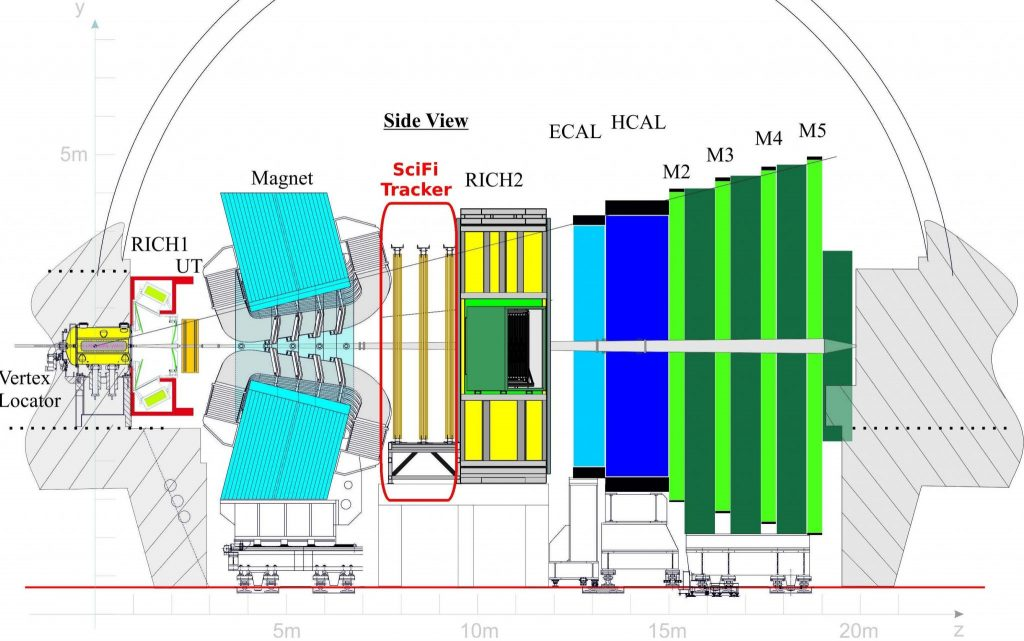
\includegraphics[width=\textwidth]{gfx/documentation/LHCb_scifi.jpeg}
        \caption{}
    \end{subfigure}
    \hfill
    \begin{subfigure}{0.48\textwidth}
        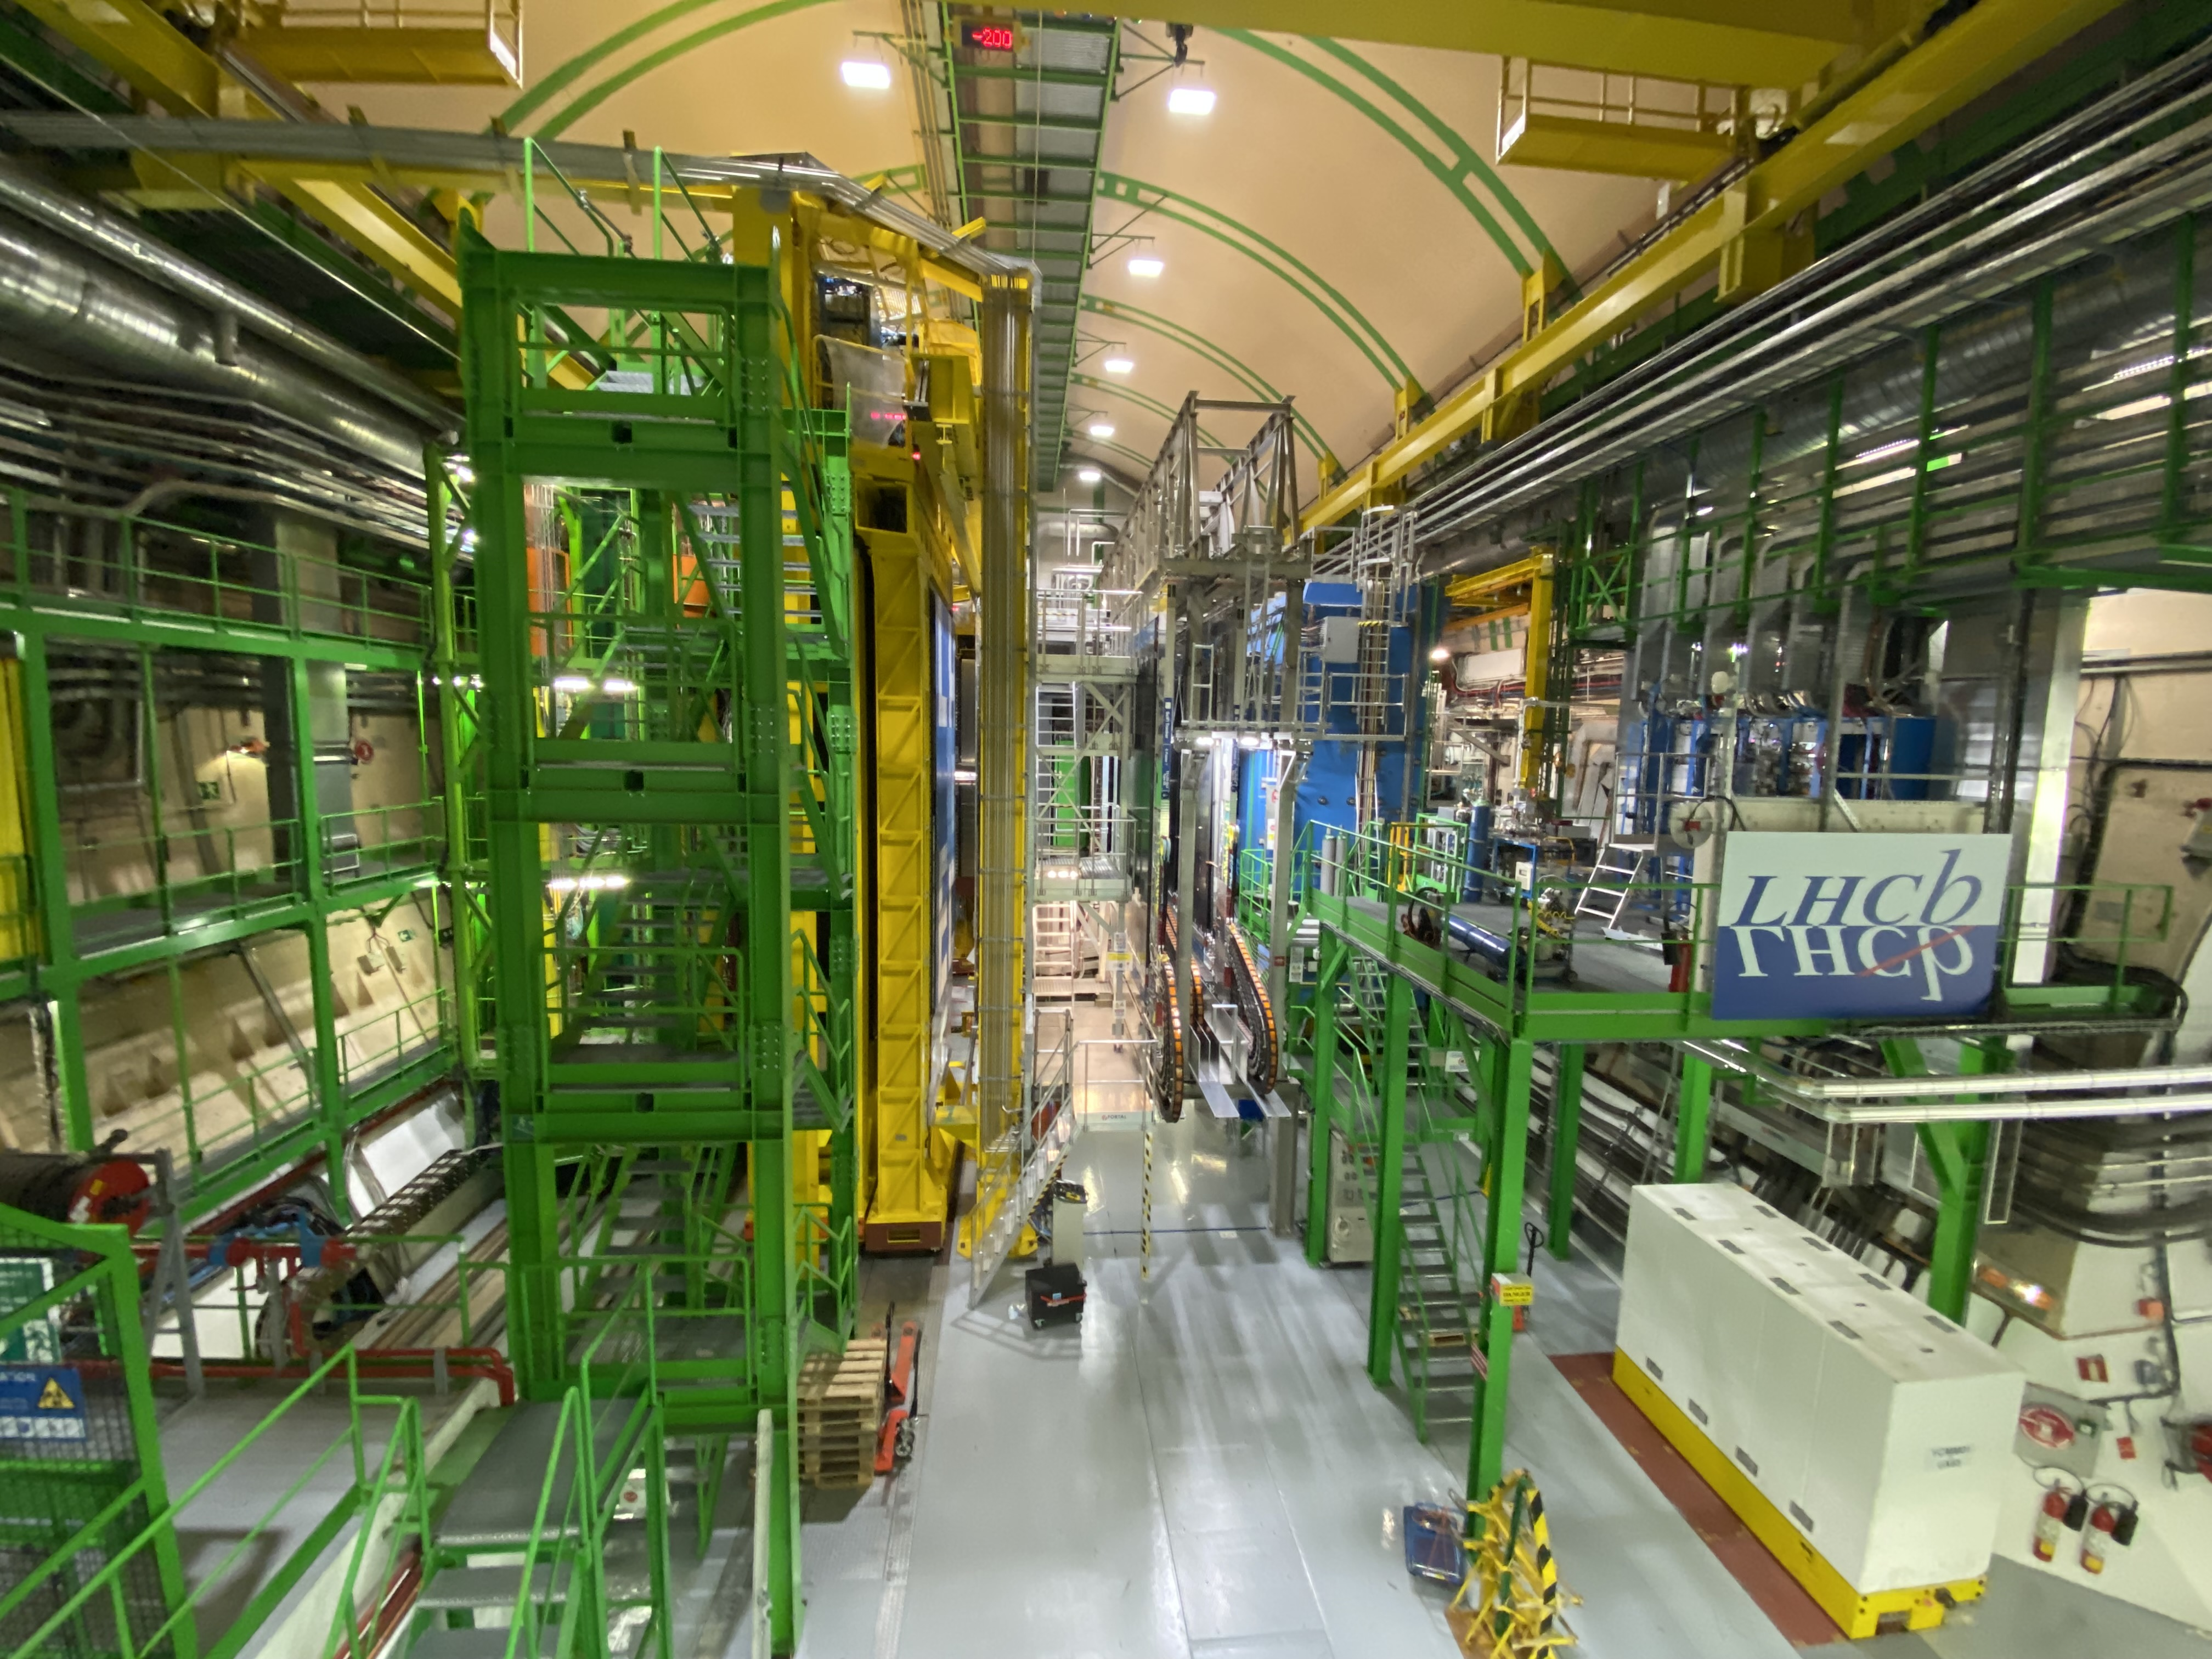
\includegraphics[width=\textwidth]{gfx/documentation/IMG_0942.jpeg}
        \caption{}
    \end{subfigure}
    \caption{LHCb detector complex with the SciFi tracker encircled in red \cite{TheEPFL} (a) and photograph of LHCb (b).}
    \label{fig:LHCb detector scheme +scifi}
\end{figure}
LHCb is made of several subdetectors, among them, the SciFi tracker made of 3 stations covering a total area of $340$ m$^2$ (see Fig. \ref{fig:scifitracker scheme}).
\begin{figure}[htbp]
    \centering
    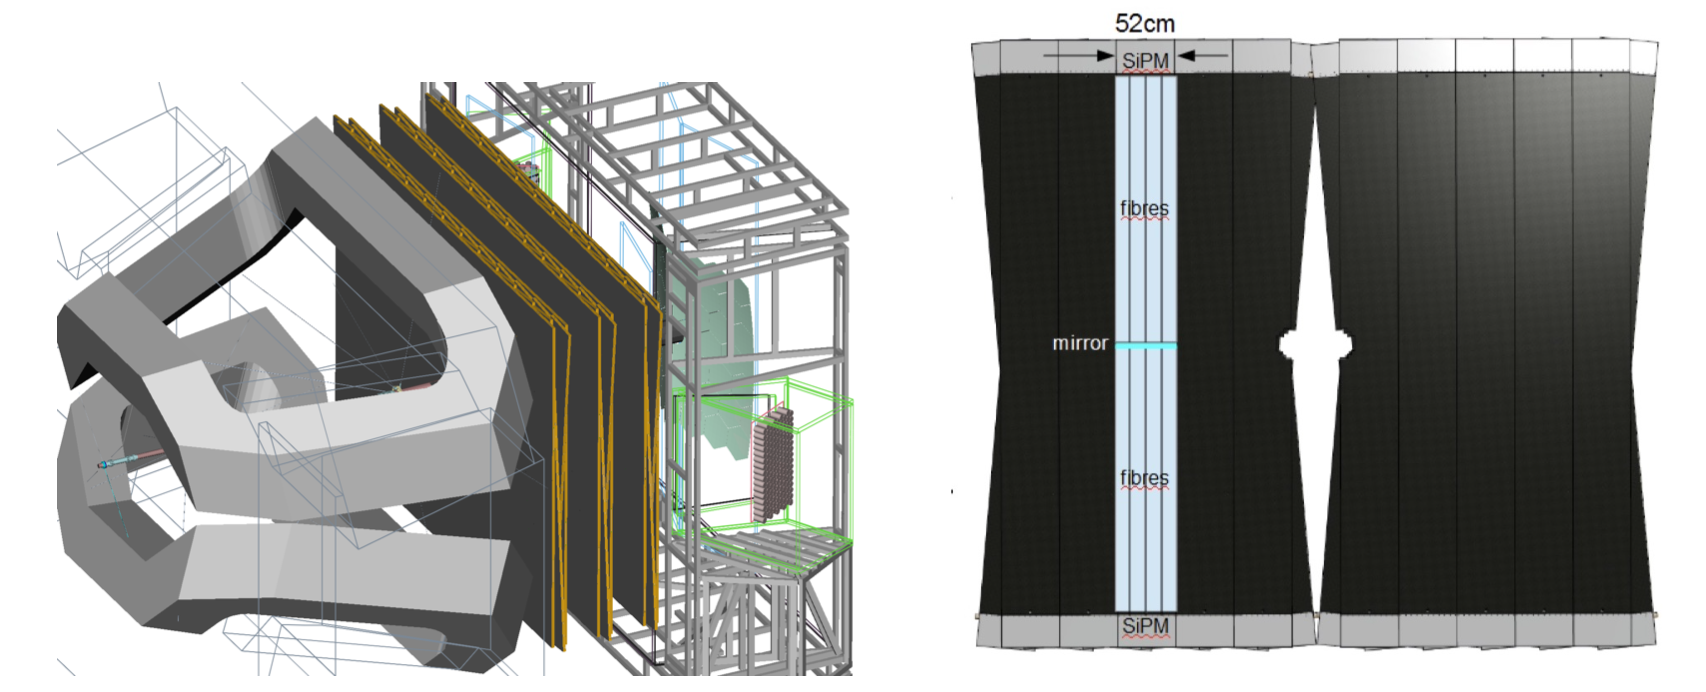
\includegraphics[width=\textwidth]{gfx/pictures/scifitracker.png}
    \caption{SciFi tracker scheme from \cite{TripplDevelopmentLHCb}.}
    \label{fig:scifitracker scheme}
\end{figure}
Each station is made of four planes oriented in different direction to obtain a spatial resolution up to \SI{100}{\micro m}. The planes are made of scintillating fibre mats. These fibres have a \SI{250}{\micro m} diameter and emit light from \SI{400}{\nano m} to \SI{600}{\nano m} with an emission peak at \SI{450}{\nano m}. SiPM arrays of \SI{250}{\micro m} summing up to $524$k channels  read out the light coming from the fibre mats. A cooling system allows to operate the SiPMs  at \SI{-40}{\celsius} in order to lower the noise due to intense radiations coming from LHC collisions. A detailed scheme shows the connection between the fibres and the SiPM in Fig. \ref{fig:fibre to sipm}.

\begin{figure}[htbp]
    \centering
    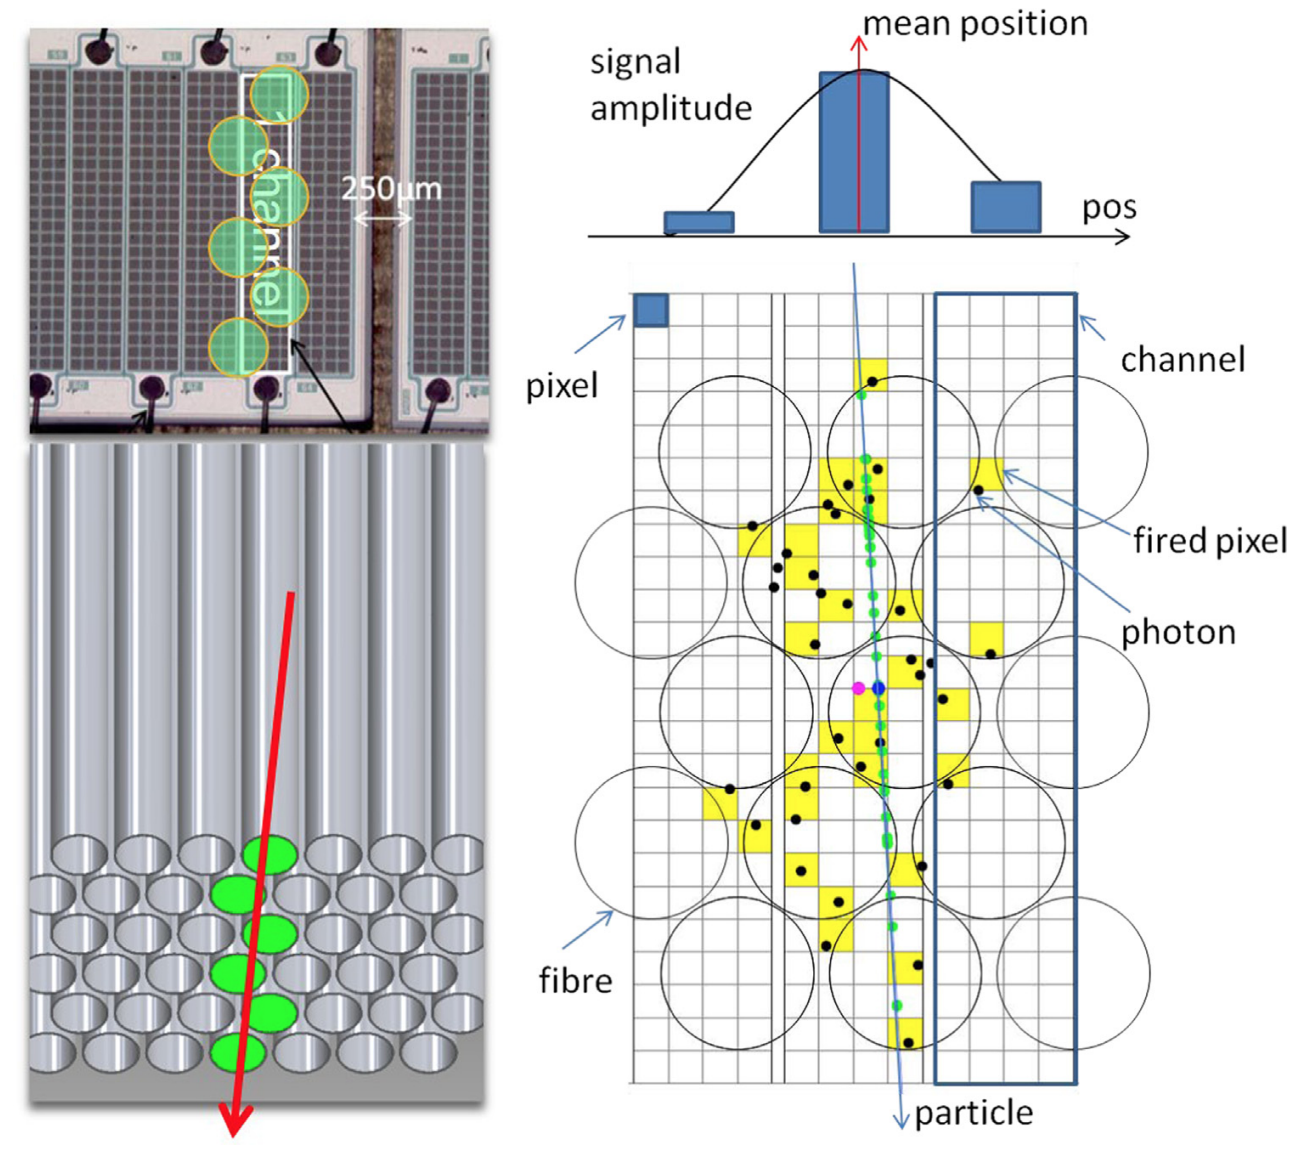
\includegraphics[width=0.9\textwidth]{gfx/pictures/fibretosipm.png}
    \caption{Scheme of the principle of the SciFi tracker. A particle hit creates photons within the fibre that are guided to the SiPM. The yellow squares represents the fired pixels the the SiPM. One can notice that there is not a one-to-one relation between a fibre and a channel (or pixel). \cite{KirnSciFi-ALHCb}.}
    \label{fig:fibre to sipm}
\end{figure}
Over time, and especially for the next LHC upgrade, where the luminosity will be increased, radiations damage the fibre in the SciFi, resulting in less light coming to the SiPMs. One way of countering this damage is to enhance the SiPM PDE either using micro lenses\cite{TripplDevelopmentLHCb}, using other SiPMs with higher PDE or both. 
A characterisation of SiPMs manufactured by the Foundation Bruno Kessler \cite{FBKKessler} is done to be used as a baseline for further R\&D about these SiPMs for the LHCb SciFi tracker.\\ 
Throughout this semester, methods for measuring the quenching resistor, breakdown voltage, correlated noise, gain and photo-detection efficiency have been implemented and adjusted to the FBK detectors.\\
\\
This thesis will firstly go into details of the working principle of a SiPMs in chapter \ref{ch:background}, then the experimental method of each measurements will be presented in chapter \ref{ch:Experimental setup and methods} and this will be followed by the presentation of the results in chapter \ref{ch:Results}.


%LPHE is responsible for providing, developing, qualifying, and testing the Silicon Photo-Multipliers (\ac{SiPM}) employed in the SciFi tracker. \ac{SiPMs} are used to readout the light emitted by the fibre mats in the tracker.\\ 

\chapter{Silicon Photo-multipliers fundamentals}
\label{ch:background}
In this chapter, the fundamentals of silicon photo-multipliers will be reviewed. The material described is focused of the physics behind the SiPM starting from the PN junction to the Diodes and then the SiPM.

%
% Section: Basic principles
%
\section{PN junctions}
\label{sec:background:Basic principles:PN junctions}
A PN junction is formed by combining two semiconductor materials which have been doped differently. Doping involves introducing impurities (group III elements for positive doping and  group V for negative doping) into the crystal structure, creating free charge carriers. The P-type semiconductor contains positive charge carriers called holes. The other material, the N-type semiconductor, has an excess of negative charge carriers called electrons. 

When a P-doped crystal is joined with an N-doped crystal, a depletion region is created by the diffusion of the charge carriers. The holes from the P-type material and the electrons from the N-type material combine. As a consequence of this recombination, positive electric charge accumulates on the N-doped side, while negative electric charge accumulates on the P-doped side. This charge generates an electric field in the depletion region and therefore a voltage, referred to as built-in voltage. One can see In Fig. \ref{fig:PN junctions scheme} a scheme of a P and N type material and a PN junction. 
\begin{figure}[htbp]
 \centering
 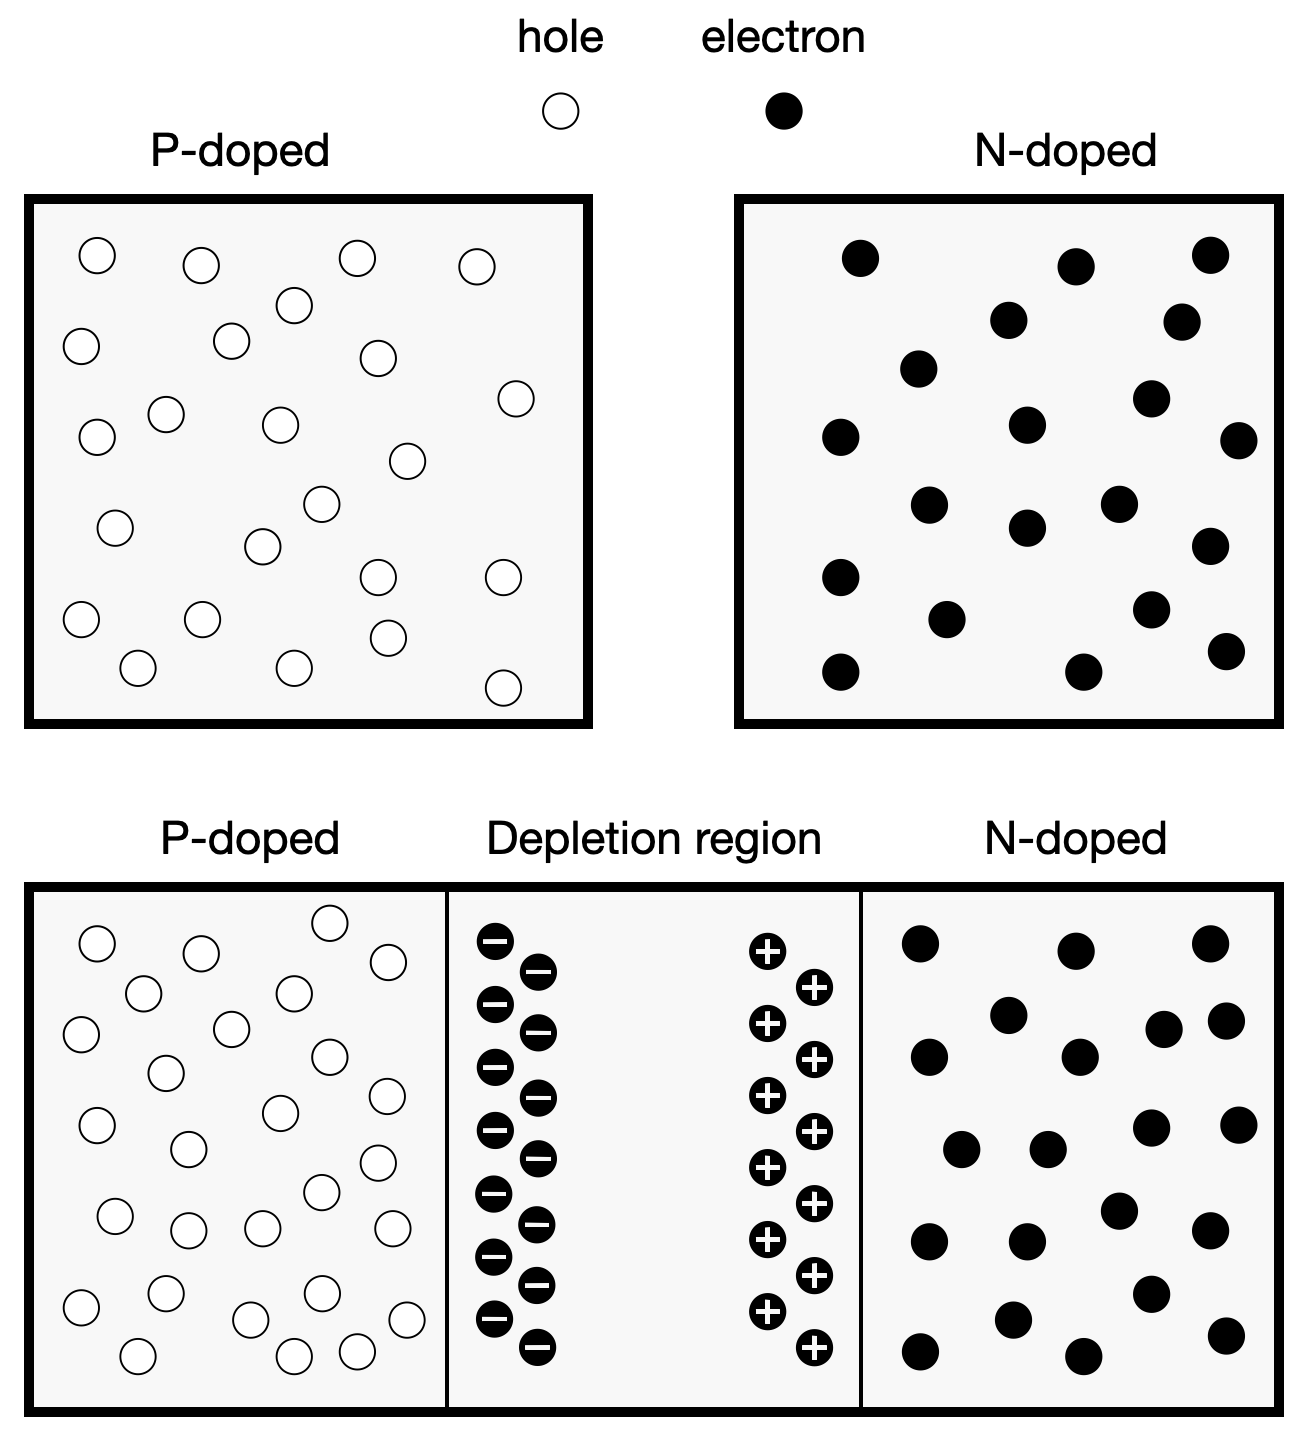
\includegraphics[width=0.6\textwidth]{gfx/schemes/PN_junction.png}
 \caption{PN junction scheme, before joining the two materials (top) and after (bottom). }
\label{fig:PN junctions scheme}
\end{figure}


\section{Diode}
\label{sec:background:Basic principles:Diodes and photo-diodes}
A diode is an electronic component made of a PN junction. 
When an external voltage is applied, we referred to it as the bias voltage $V_{bias}$, the size of the depletion region can vary and so the diode current. The IV characteristic curve of a diode is shown in Fig. \ref{fig:chapter02:Diodes and photo-diodes: iv curve}. Depending on the direction of the bias voltage, one can see different behaviors, and define the different operation modes. 
\begin{figure}[htbp]
 \centering
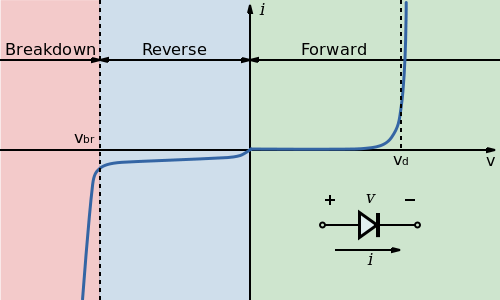
\includegraphics[width=0.7\textwidth]{gfx/documentation/Diode_IV_curve.png}
 \caption{Diode IV characteristic curve \cite{DiodeCurve}.}
 \label{fig:chapter02:Diodes and photo-diodes: iv curve}
\end{figure}


\paragraph{Forward Bias mode.} Forward bias means that the voltage applied reduces the width of the depletion region. The cathode is connected to the P-type and the anode to the N-type of the junction. More electrons will recombine with the holes in the P doped region, and holes will recombine in the N-type resulting in a smaller depletion.

\paragraph{Reverse Bias mode.} When a diode is in Reverse Bias mode, the cathode is connected to the N side (anode to the P side). Holes are attracted to the negatively charged end of the generator and electrons to the positively charged end resulting in a larger depletion region. 

\paragraph{Breakdown.} 
The breakdown voltage $V_{bd}$ is the bias voltage value where any free charge carrier in the depletion region is sufficiently accelerated by the electric field so that it triggers an avalanche. A single electron-hole pair can create a self-sustaining electron-hole avalanche. The regime of operation beyond the breakdown voltage ($V_{bias} > V_{bd}$) is often called Geiger-Mode and we can define a quantity named overvoltage $\Delta V = V_{bias}-V_{bd}$ for this regime.


\subsection{Photodiode}
\label{ch:2:subsec:Photodiode}
The standard photodiode is a PN junction. When a photon enters the detection area (depletion region), it can interact by photo-electric effect and create an electron-hole pair. If the diode is not biased, this electron pair will generate a small tension and behaves like a solar cell. Photodiodes are employed to measure light sources big enough so that the current produced is measurable. They are not suited to detect single photons. 

\subsection{Avalanche photodiode}
\label{ch:2:subsec:Avalanche photodiode}
An \ac{APD} is reverse biased but the electric field's intensity is high enough so that the electron can gain enough speed to ionise other atoms in the crystal and triggering a chain reaction or avalanche. Due to their higher effective mass, the holes are not accelerated enough to create an electron-hole avalanche because APDs operate below breakdown voltage. 

\section{Single Photon Avalanche Diodes}
\label{sec:background:Basic principles:SPADs}
\ac{SPAD} or \ac{G-APD} is an Avalanche Photo-diode operating in Geiger-Mode, meaning that the bias voltage is above the breakdown voltage. This specificity allows this device to detect single photons, since one pair of electron-hole can trigger a self-sustaining avalanche and then generate an electric current intense enough to be measured. Due to the exponential growth of the current generated, if nothing is done the quench it, the diode can be damaged or even burned. The quenching resistor $R_Q$ is introduced to prevent the diode from burning. When the photo-current $I_{ph}$ increases, the voltage at the ends of the resistor $R_Q$ increases (because $V_{R_Q}= R_Q\cdot I_{ph}$). By the law of mesh $V_{bias} + V_{diode}+ V_{R_Q} = 0$, hence $V_{diode}$ decreases as $V_{R_Q}$ increases. The voltage $V_{diode}$ will drop below $V_{bd}$ and the avalanche created will not be self-sustaining. The avalanche is then quenched.

\begin{figure}[htbp]
 \centering
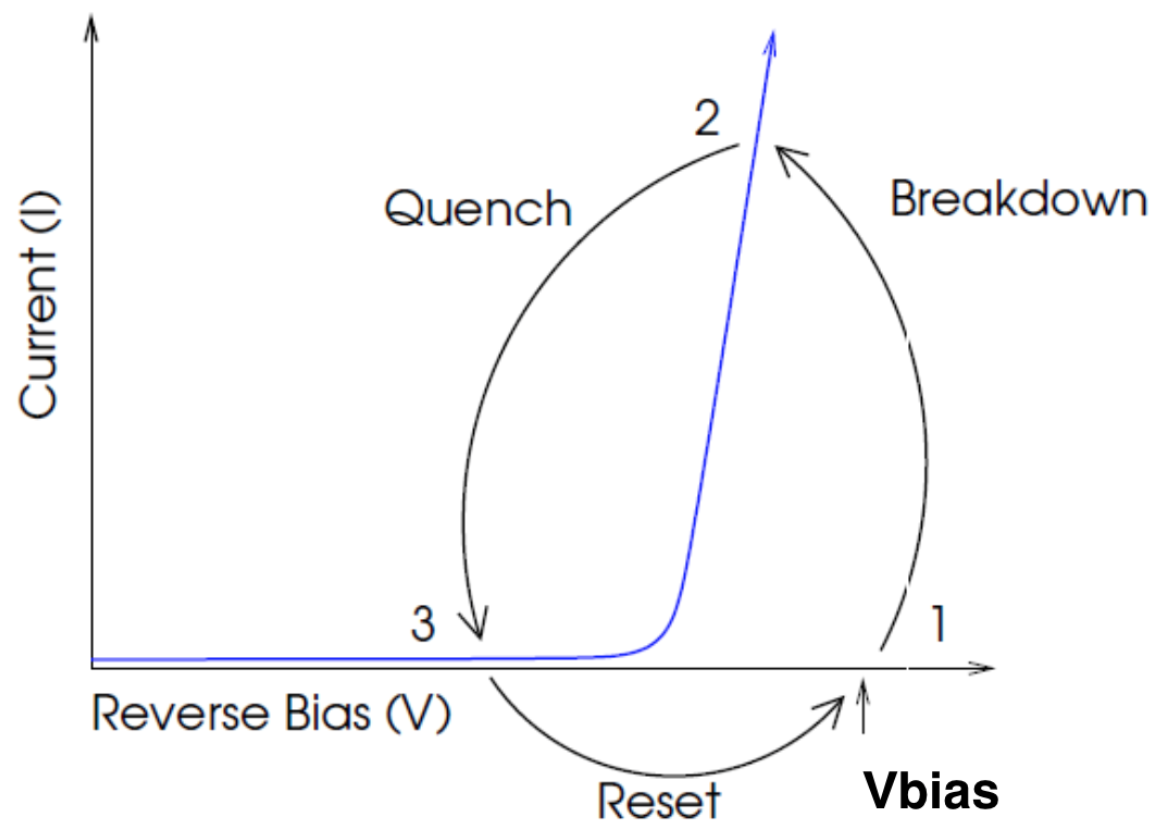
\includegraphics[width=0.7\textwidth]{gfx/documentation/switch_analogy.png}
 \caption{SPAD response as function of $V_{bias}$. 
 \cite{Onsemi2021IntroductionMultipliers}
 }
\label{fig:chapter02:Diodes and photo-diodes:switch}
\end{figure}
The working principle is shown in Fig. \ref{fig:chapter02:Diodes and photo-diodes:switch}. 
When a photon is detected, an avalanche is triggered and then quenched. During this time, the SPAD recharges, avalanches could still be triggered, but will be smaller until the SPAD recharges. This time is defined as the recovery time $\tau_{rec}$. We can define another time constant of the pulse shape $\tau_{long}$ that corresponds to the time it takes for the signal to go down to the baseline and it is equal to the recovery or recharging time $\tau_{rec}$. A SPAD can detect single photons, but it will not be able to distinguish between two or more photons that hit within the recharging time. Once the avalanche is triggered, a second photon hit will not result in an avalanche twice as big. Nevertheless, there is a way to detect multiple photons, by adding several SPADs in parallel and form a SiPM.  
\begin{figure}[htbp]
    \centering
    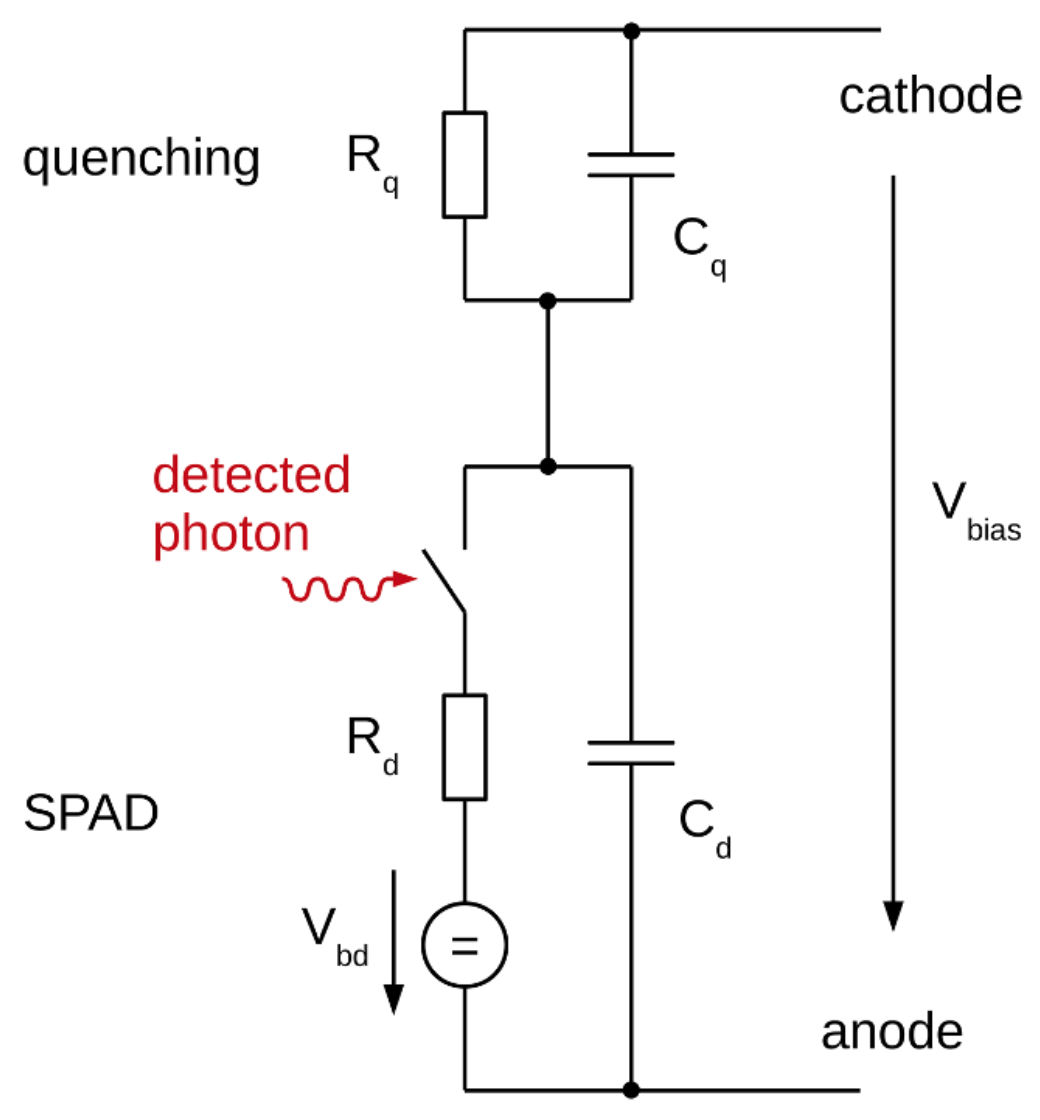
\includegraphics[width=0.48\textwidth]{gfx/documentation/spad_circuit.png}
    \caption{SPAD electronic circuit equivalent, with integrated quenching circuit. 
    \cite{Gundacker2020TheDetector}}
\end{figure}


\section{Silicon Photo-Multiplier}
\label{sec:background:SiPMs}
The SiPM is a solid-sate photodetector made of multiple SPADs connected in parallel. It can detect multiple photons at once if they hit different pixels. One can see the electronic circuit of an example of SPAD array composing a SiPM.
\begin{figure}[htbp]
    \centering
    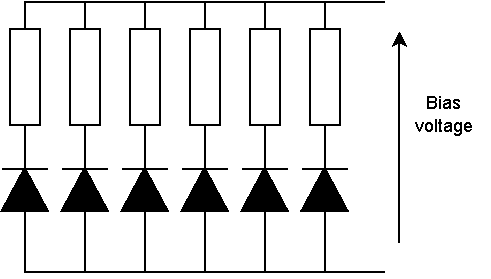
\includegraphics[width=0.5\textwidth]{gfx/schemes/sipm.drawio.pdf}
    \caption{SiPM electronic circuit equivalent with the SPADs connected in parallel.}
    \label{fig:chapter02:Sipm:electronic scheme}
\end{figure}


\subsection{Pixel or Micro-Cell}
\label{subsec:Pixel or Micro-Cell}
\begin{wrapfigure}[12]{r}{0.4\textwidth}
    \centering
    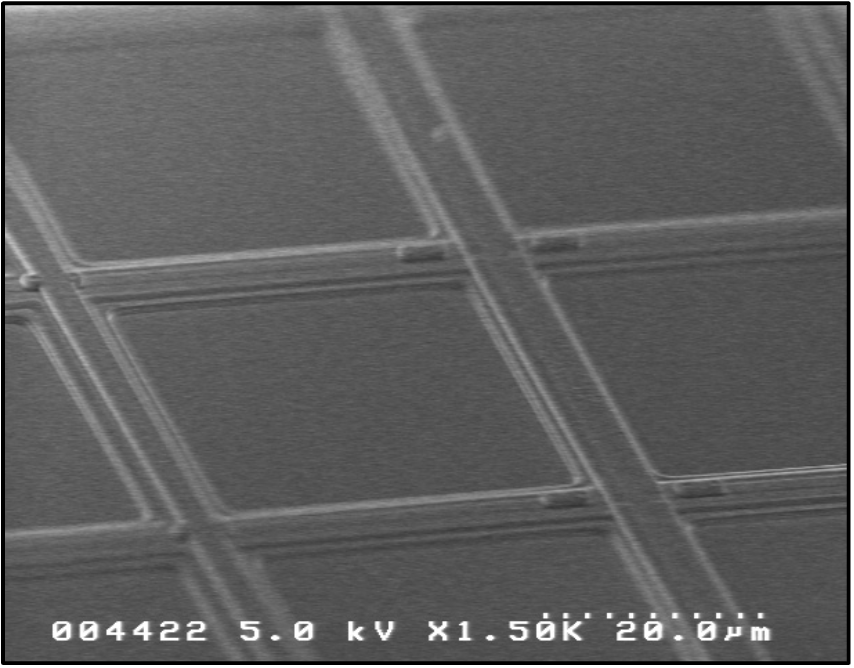
\includegraphics[width=0.4\textwidth]{gfx/documentation/pixel_pic.png}
    \caption{Image of a pixel structure on a SiPM \cite{Onsemi2021IntroductionMultipliers}.}
    \label{fig:chapter02/sipm/pixel pic}
\end{wrapfigure}
In a SiPM, each SPAD is a pixel (or micro-cell). The structure of a pixel, including its active and inactive areas, is depicted in Fig. \ref{fig:chapter02/sipm/pixel pic} where the internal square is the active area. The borders contain the trenches, quenching resistors and referred to as the inactive area. When designing a SiPM, manufacturers can produce SiPMs with different number of pixels and pixel sizes. For a given detector size, these two parameters have advantages and drawbacks. 
Increasing the number of pixels while maintaining a constant detector size enhances the dynamic range. The dynamic range can be analogously understood as the resolution of the detector, a smaller dynamic range reduces the chances that two close photons hit two different pixels.
However, with smaller pixels, the two photons might hit separate pixels, enabling their individual counting.
There is a trade-off when increasing the number of pixels, as it also increases the inactive area. This inactive area consists of components such as quenching resistors, trenches, metal guards, etc. The ratio between the active area and the total area is defined as the \ac{FF}. The FF significantly influences the PDE, as explained below in \ref{subsection:PDE}.
Therefore, for a detector of the same size, increasing the number of pixels enhances the dynamic range but reduces the gain and PDE and vice versa.


\subsection{Gain}
\label{subsection:Gain}
The gain of a SiPM is defined as the amount of electron-hole pairs generated in an avalanche. It represents the avalanche size and is proportional to the active volume in the pixel.
The gain is computed as in Eq. \eqref{eq:gain theory} (where $C_d$ is the pixel capacitance): 
\begin{equation}
    G= \frac{C_d \cdot \Delta V}{e}
    \label{eq:gain theory}
\end{equation}


\subsection{Photo-detection efficiency }
\label{subsection:PDE}
PDE is a key characteristic of a SiPM and defines the probability that a photon is converted into signal. This quantity depends on several parameters, such as the wavelength of the detected photons $\lambda$ or the overvoltage $\Delta V$. The formula is usually of the form:
\begin{equation}
      PDE(\lambda, \Delta V)= \eta(\lambda)\cdot \varepsilon(\Delta V)\cdot FF  
    \label{eq:pde theory}
\end{equation}
where $\eta(\lambda)$ is the quantum efficiency of the cell, which is the probability that a photon generates an electron-hole pair.   $\varepsilon(\Delta V)$ is the avalanche triggering probability and $FF$ the Fill Factor. 
% Vbd, R_Q, Gain, PDE

\subsection{Dark count and correlated noise}
\label{subsec:Correlated noise}
The avalanche triggering is not necessarily from a photon, an electron-hole pair can be created by thermal excitation resulting in noise. 
\paragraph{Dark count} Dark Counts or Dark Current are the primary source of noise in the SiPM. Some free charge carriers can be generated in the depletion region due to thermal excitation. Since the SiPM operates above $V_{bd}$, any single charge carrier can generate an avalanche.The pulse amplitude a of dark count is $1$\ac{PE} since only one pixel is fired. 

\paragraph{Optical Direct Cross talk} During an  avalanche, the accelerated electrons can emit photons by Bremsstrahlung effect. Those photons can travel and hit other pixels close by and in turn generate another avalanche. Hence the total signal will be the combination of the primary avalanche and the secondary avalanche from the Bremsstrahlung photon. Due to the small spatial distance between the pixels, there is approximately no delay between the signal from the primary photon and from the cross-talk photon, resulting in a 2PE peak. This type of noise is called \ac{DiXT} and we can see an example In Fig. \ref{fig:chapter02:Sources of noise}. First order DiXT is $2$PE in amplitude because two pixels are fired. There exist higher order DiXT corresponding to the number of pixels in the neighborhood fired but these are less common. 

\paragraph{Optical Delayed Cross talk}
\ac{DeXT} occurs when a photon from an avalanche generates an electron-hole pair outside the depletion region. Usually they will recombine but there is a probability that they don't. In this case, the charge carriers may drift towards the depletion region within a significant time interval. Once in the depletion region, they can trigger an avalanche in the other pixel resulting in a signal corresponding to a single photon detection with a $1$PE amplitude. 
% band gaps traps definition 

\paragraph{External Cross talk} External Cross talk is when a photon from an avalanche in one pixel is reflected by an additional coating on the top of the SiPM. This reflected photon can hit other pixels and generate this noise. In Fig. \ref{fig:all different cross talks} the different cross talk mechanisms are shown. 

\begin{figure}[htbp]
    \centering
    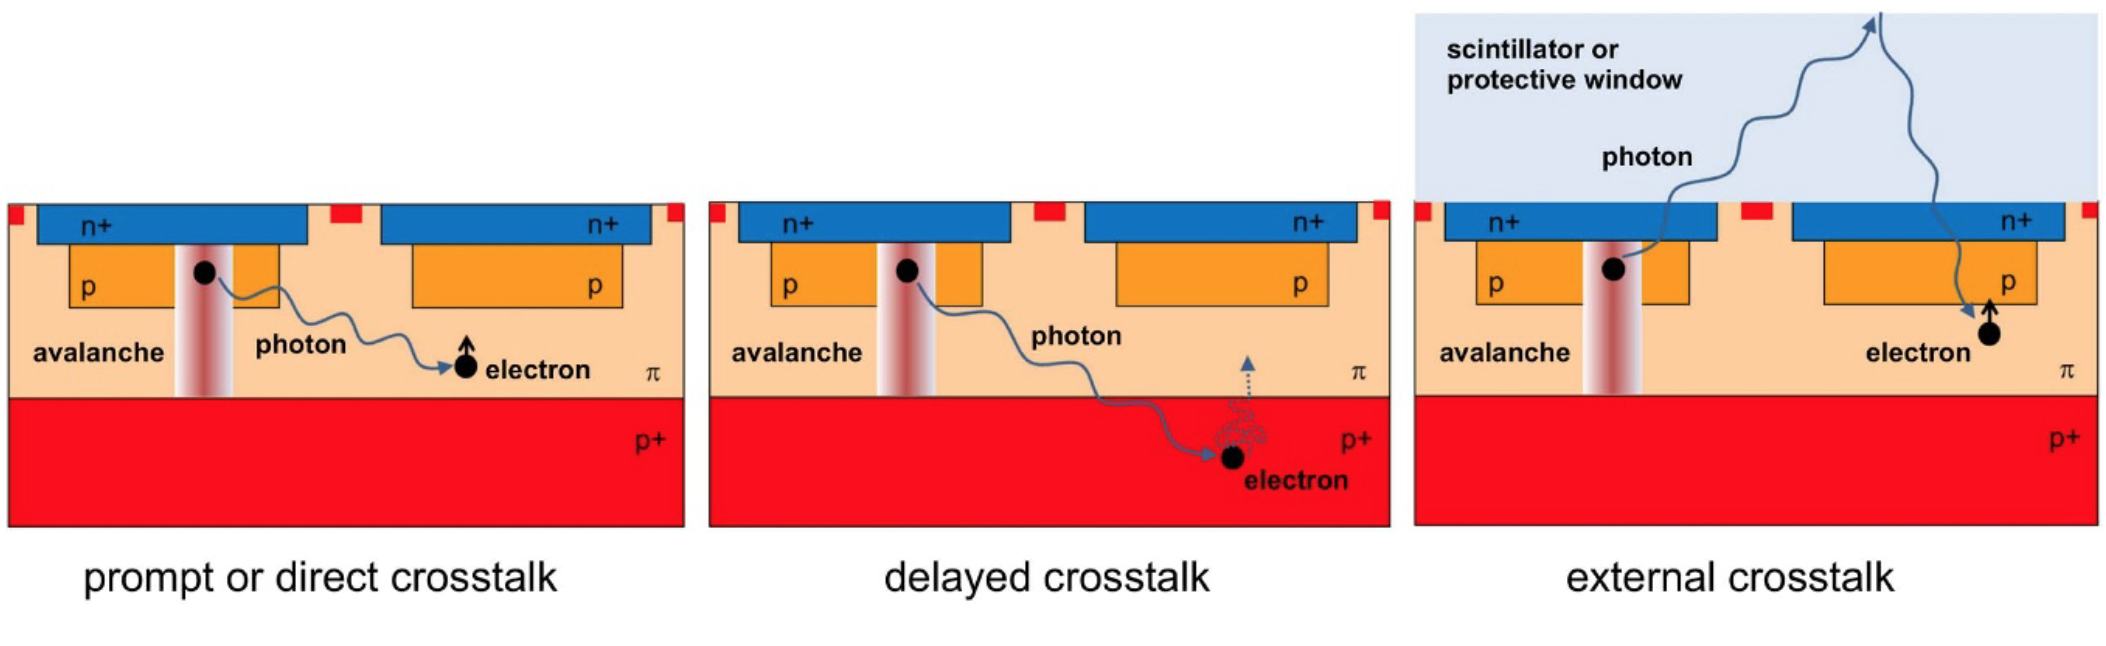
\includegraphics[width=\textwidth]{gfx/schemes/external_xTs.png}
    \caption{The three cross talk mechanisms in a SiPM \cite{ClaudioPiemonte2013PerformanceApplication}.}
    \label{fig:all different cross talks}
\end{figure}

\paragraph{After pulse}
The silicon crystal in the depletion region can have defects in their structure causing a change in the bands structure with a creation of a new level. An additional level, called a trap, may be created below the conduction band and can receive charge carriers created during a avalanche. After some time, the trapped charge carrier could be released by different effects such as thermal excitation or tunneling. Since the trap is in the depletion region, the now free charge carrier will be accelerated and may trigger an avalanche. 
\begin{figure}[htbp]
    \centering
    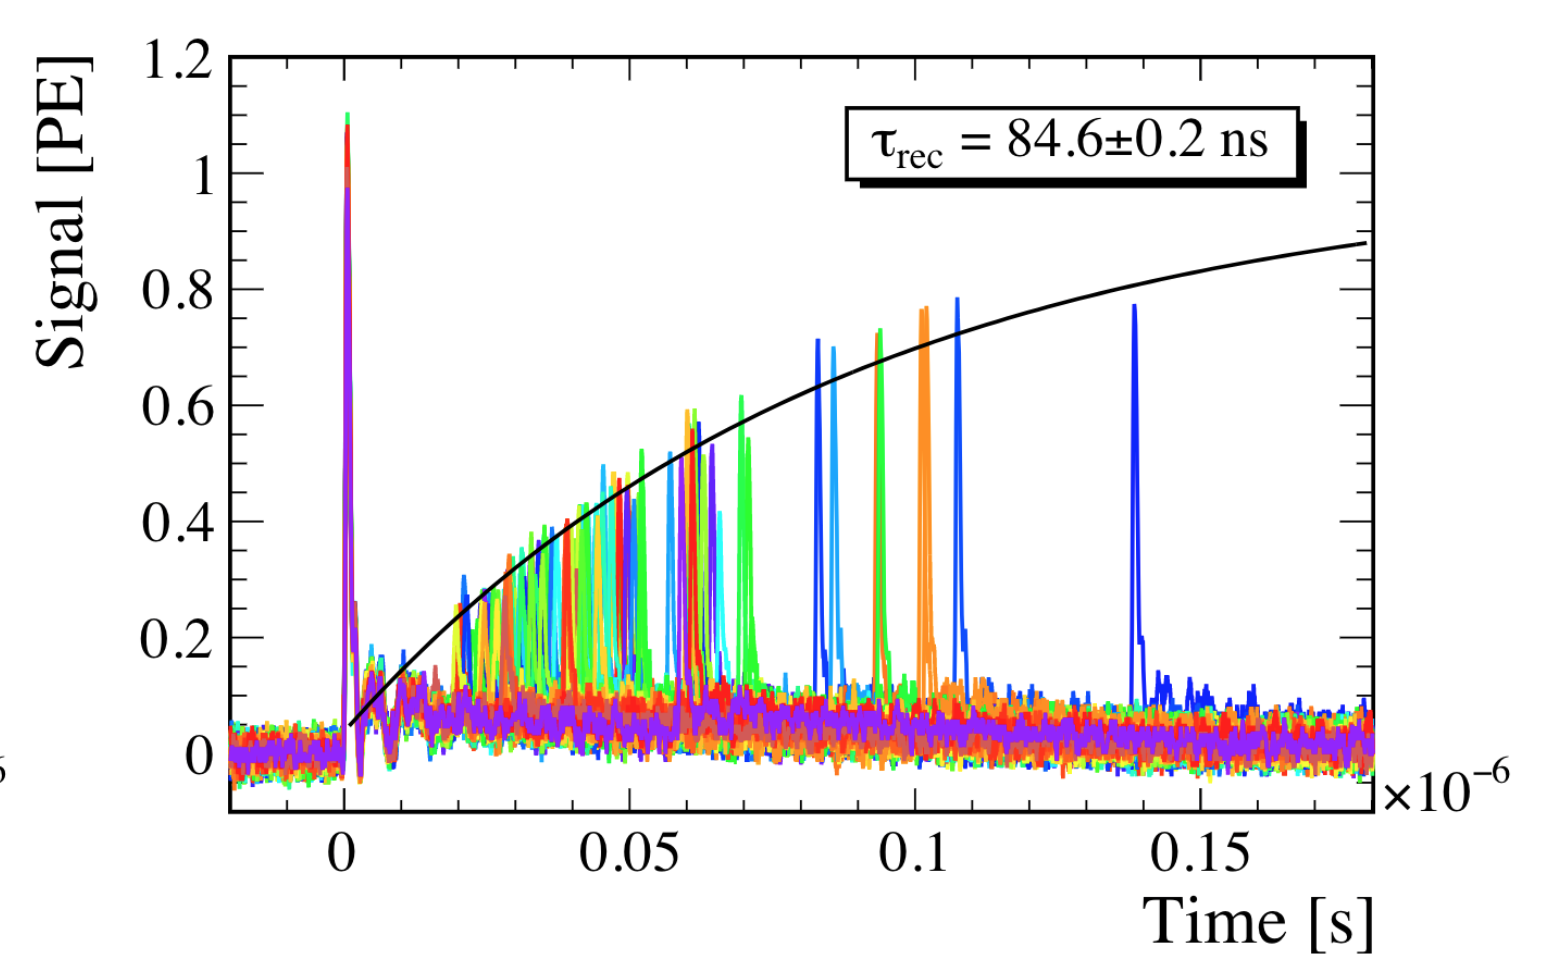
\includegraphics[width=0.6\textwidth]{gfx/documentation/afterpulse_example.png}
    \caption{Example of different after pulse shape and the fit of their amplitude, allowing to find $\tau_{rec}$. 
    \cite{Girard2018CharacterisationDistributions}}
  \label{fig:chapter02:Sources of noise: after pulse signal ex}
\end{figure}
The avalanche intensity will depend on the release time of the charge carrier meaning that the after pulse \ac{AP} signal can have different amplitude varying from $0$ to $1$ \ac{PE}. One can measure the recovery time $\tau_{rec}$ as shown in Fig. \ref{fig:chapter02:Sources of noise: after pulse signal ex}

\begin{figure}[htbp]
    \centering
    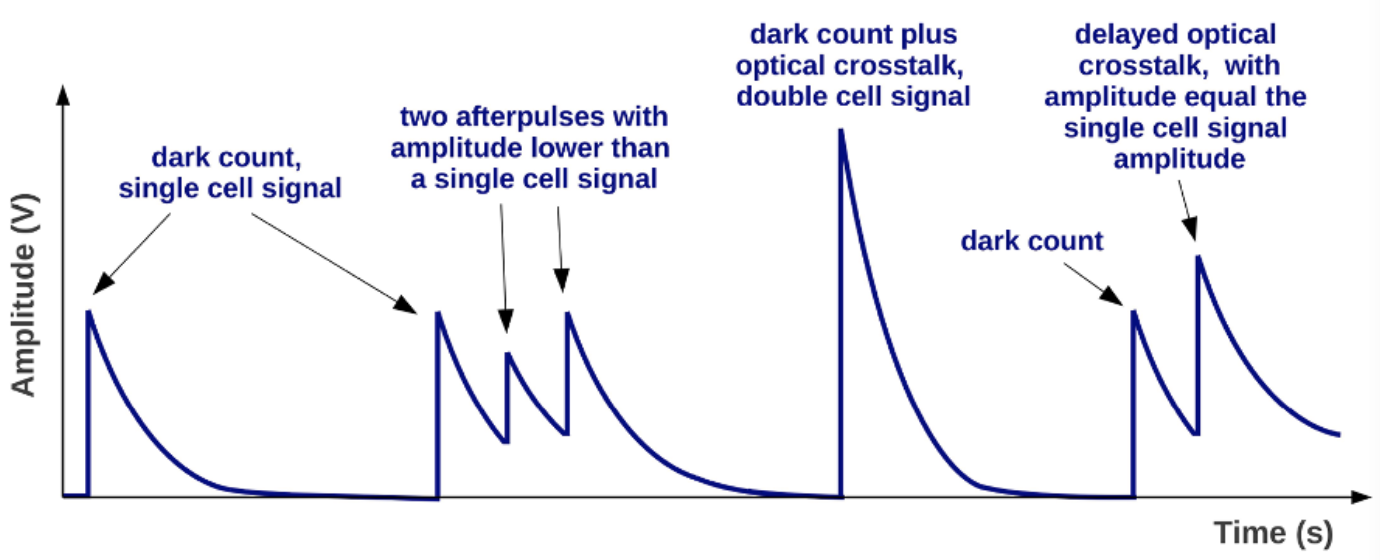
\includegraphics[width=0.9\textwidth]{gfx/documentation/noise_shapes.png}
    \caption{Example of different kind of noises shapes, and identification. 
    \cite{Gundacker2020TheDetector}
    }
    \label{fig:chapter02:Sources of noise}
\end{figure}

\section{Characterised detectors}
\label{ch:background:SiPM:characterised detectors}
This work studies three different detectors from FBK and one from Hamamatsu. 
\\
All SiPM arrays are composed of $128$ channels of \SI{250.4}{\micro m} wide. More specifications about these detectors are shown in Table \ref{table:detector specs}. A high definition picture of a SiPM from FBK is shown in \ref{fig:SiPM FBK}.
\begin{figure}[htbp]
    \centering
    \rotatebox{-90}{\includegraphics[width=0.35\textwidth]{gfx/pictures/SiPMarray.jpg}}
    \caption{128 channel SiPM array from FBK. Taken with a Keyance optical microscope, by G. Haefeli. }
    \label{fig:SiPM FBK}
\end{figure}
The Hamamatsu H2017, and the FBK \SI{31}{\micro m} \& \SI{42}{\micro m} have the same dimensions since they are designed to read out the light from the SciFi tracker. Another sample of the FBK \SI{31}{\micro m} is studied with an additional epoxy layer on the top of the sensitive area. 
\\
The characterised SiPMs from FBK are all from the same wafer, shown in Fig. \ref{fig:picture wafer} (a). In Fig. \ref{fig:picture wafer} (b), the SciFi A \& B correspond to the \SI{31}{\micro m} pixel size. The SciFi B is not analysed in this work. SciFi C is the SiPM with the largest pixel size of all three from FBK with \SI{42}{\micro m}. The \SI{16}{\micro m} (the one denoted \ac{ECAL} In Fig. \ref{fig:picture wafer} (b)) has a channel height bigger than the other ones because its use has a different purpose. In the ECAL, the fibre mats has a larger thickness, hence the choice of having SiPMs wider to collect all the photons. The Hamamatsu detector's breakdown voltage has a temperature dependency of \SI{54}{\milli \volt. \per \celsius}\cite{HamamatsuPhotonicsHowPhotonics} whereas the FBK have \SI{32}{\milli \volt. \per \celsius}.

\begin{table}[h]
\centering
\begin{tabular}{|l|l|l|l|l|l|}
\hline
\textbf{SiPM}               & \textbf{H2017} & \textbf{FBK \SI{16}{\micro m}} & \textbf{\begin{tabular}[c]{@{}l@{}}FBK \SI{31}{\micro m} \end{tabular}}  & \textbf{FBK \SI{42}{\micro m}} \\ \hline
\textbf{Pixel size [\SI{}{\micro m}]}         &    $57.5 \texttt{x}62.5$ &  $15.65$   &  $31.3$ &   $41.733$           \\ \hline
\textbf{$N_{pixel}$ (per channel)}        &  $104$   &    $3072$    &  $424$    &     $234$    \\ \hline
\textbf{Channel active height [\SI{}{\micro m}]}     & $1658.9$  &   $3004.8$  &  $1658.9$  & $1627.6$   \\ \hline
\end{tabular}
\caption{Specifications of the studied detectors.}
\label{table:detector specs}
\end{table}

\begin{figure}[htbp]
  \centering
  \begin{subfigure}[b]{0.48\linewidth}
    \centering
    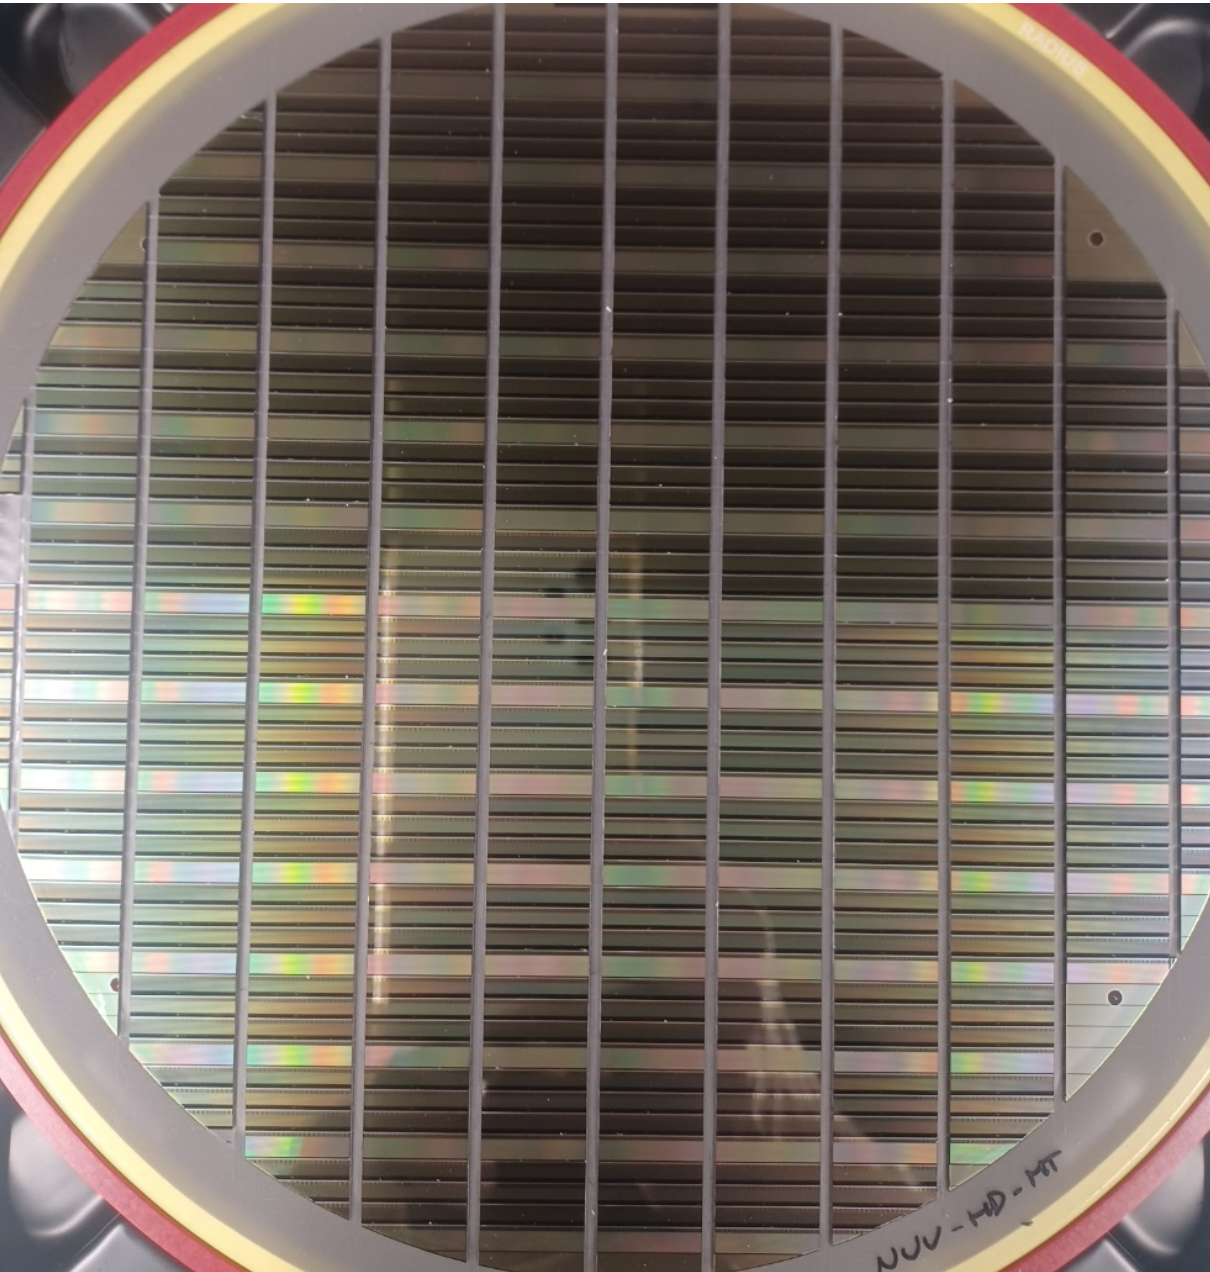
\includegraphics[width=0.9\linewidth]{gfx/pictures/Wafer.png}      
    \caption{}
  \end{subfigure}
  \hfill
  \begin{subfigure}[b]{0.48\linewidth}
    \centering
    \hspace{0.5cm}
    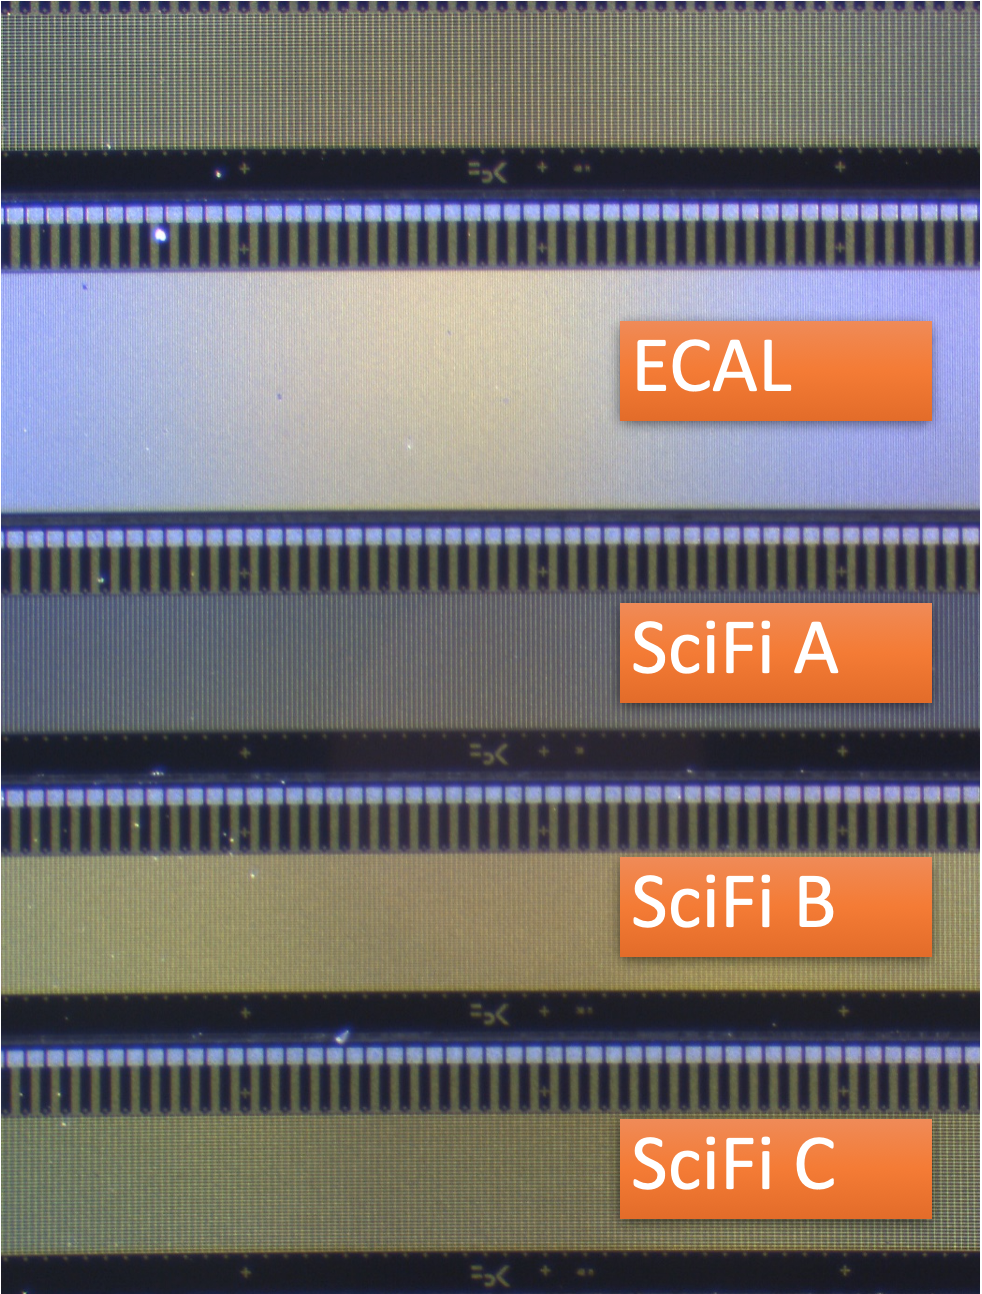
\includegraphics[width=0.7\linewidth]{gfx/pictures/FBK_types_Wafer.png}
    \caption{}    
  \end{subfigure}
    \caption{Picture of the FBK wafer containing the 4 types of detectors (a) and zoomed in picture of the 4 detectors types (b).}
    \label{fig:picture wafer}
\end{figure}

\subsection{Hamamatsu and FBK technology}
\label{ch:background:SiPM:characterised detectors:FBKvsH}

\paragraph{FBK NUV-HD technology}
The FBK \ac{NUV-HD} technology has been designed to have a high dynamic range, low correlated noise and to be used in cryogenic applications. The pixel edges contains a trench between active areas (in grey Fig. \ref{fig:fbk tech scheme trench photo} (a)) of less than \SI{3}{\micro m}. They reduce the probability of cross talk while limiting the dead space. A micro graph of these deep trenches can be seen in Fig. \ref{fig:fbk tech scheme trench photo} (b). The integrated poly-silicon quenching resistor can been In Fig. \ref{fig:fbk tech scheme trench photo} (a). An annotated picture of the FBK pixel is shown in \ref{fig:fbk tech scheme trench photo} (c) where the metal guards are visible. 
\begin{figure}[htbp]
  \centering
  \begin{subfigure}[b]{0.48\linewidth}
    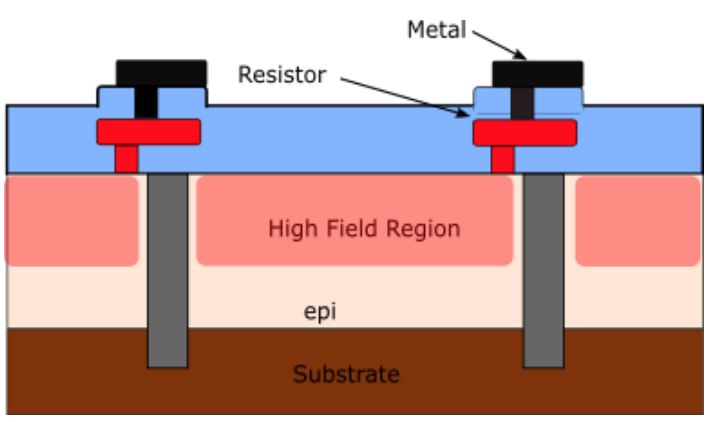
\includegraphics[width=1\linewidth]{gfx/schemes/FBK_technology_spad.png}
    \caption{}  
  \end{subfigure}
  \hfill
  \begin{subfigure}[b]{0.48\linewidth}          
    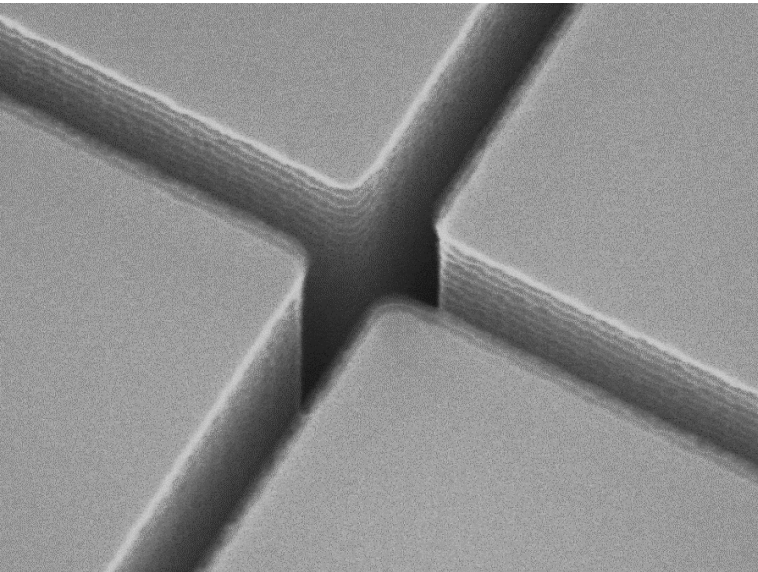
\includegraphics[width=1\linewidth]{gfx/pictures/FBK_trench.png}  
    \caption{}
  \end{subfigure}
  \hfill
  \begin{subfigure}[b]{1\linewidth}          
    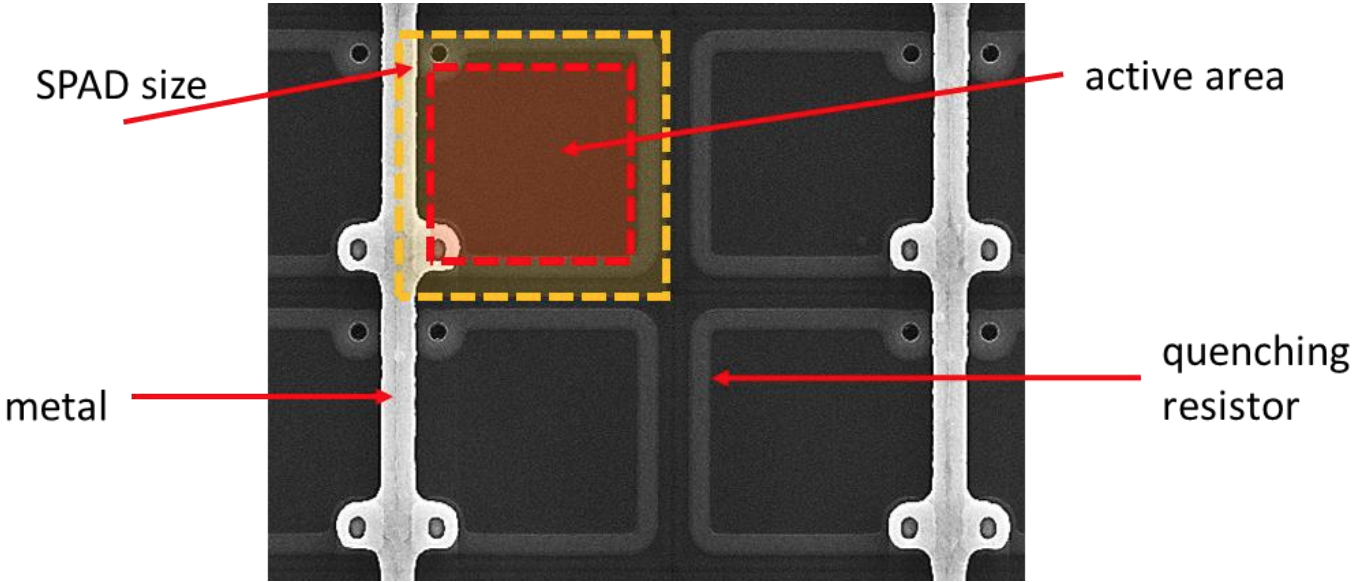
\includegraphics[width=1\linewidth]{gfx/pictures/FBK_techpic.png} 
    \caption{}
  \end{subfigure}
    \caption{Scheme of FBK cell (a) and photograph of FBK deep trenches between pixels (b) and view from above (c). \cite{Paternoster2019SiliconPerspectives}}
    \label{fig:fbk tech scheme trench photo}
\end{figure}


\paragraph{Hamamatsu technology}
A picture of the H2017 pixels shows the structure of this detector (see Fig. \ref{fig:H2017 pixels picture guido}). As in the FBK, trenches between the pixels are visible. On the Hamamatsu the $R_Q$ is composed of a thin transparent film on the active surface where as the FBK $R_Q$ is made of poly silicon. More informations about this detector can be found in \cite{SurfaceArray}.
\begin{figure}[htbp]
    \centering
    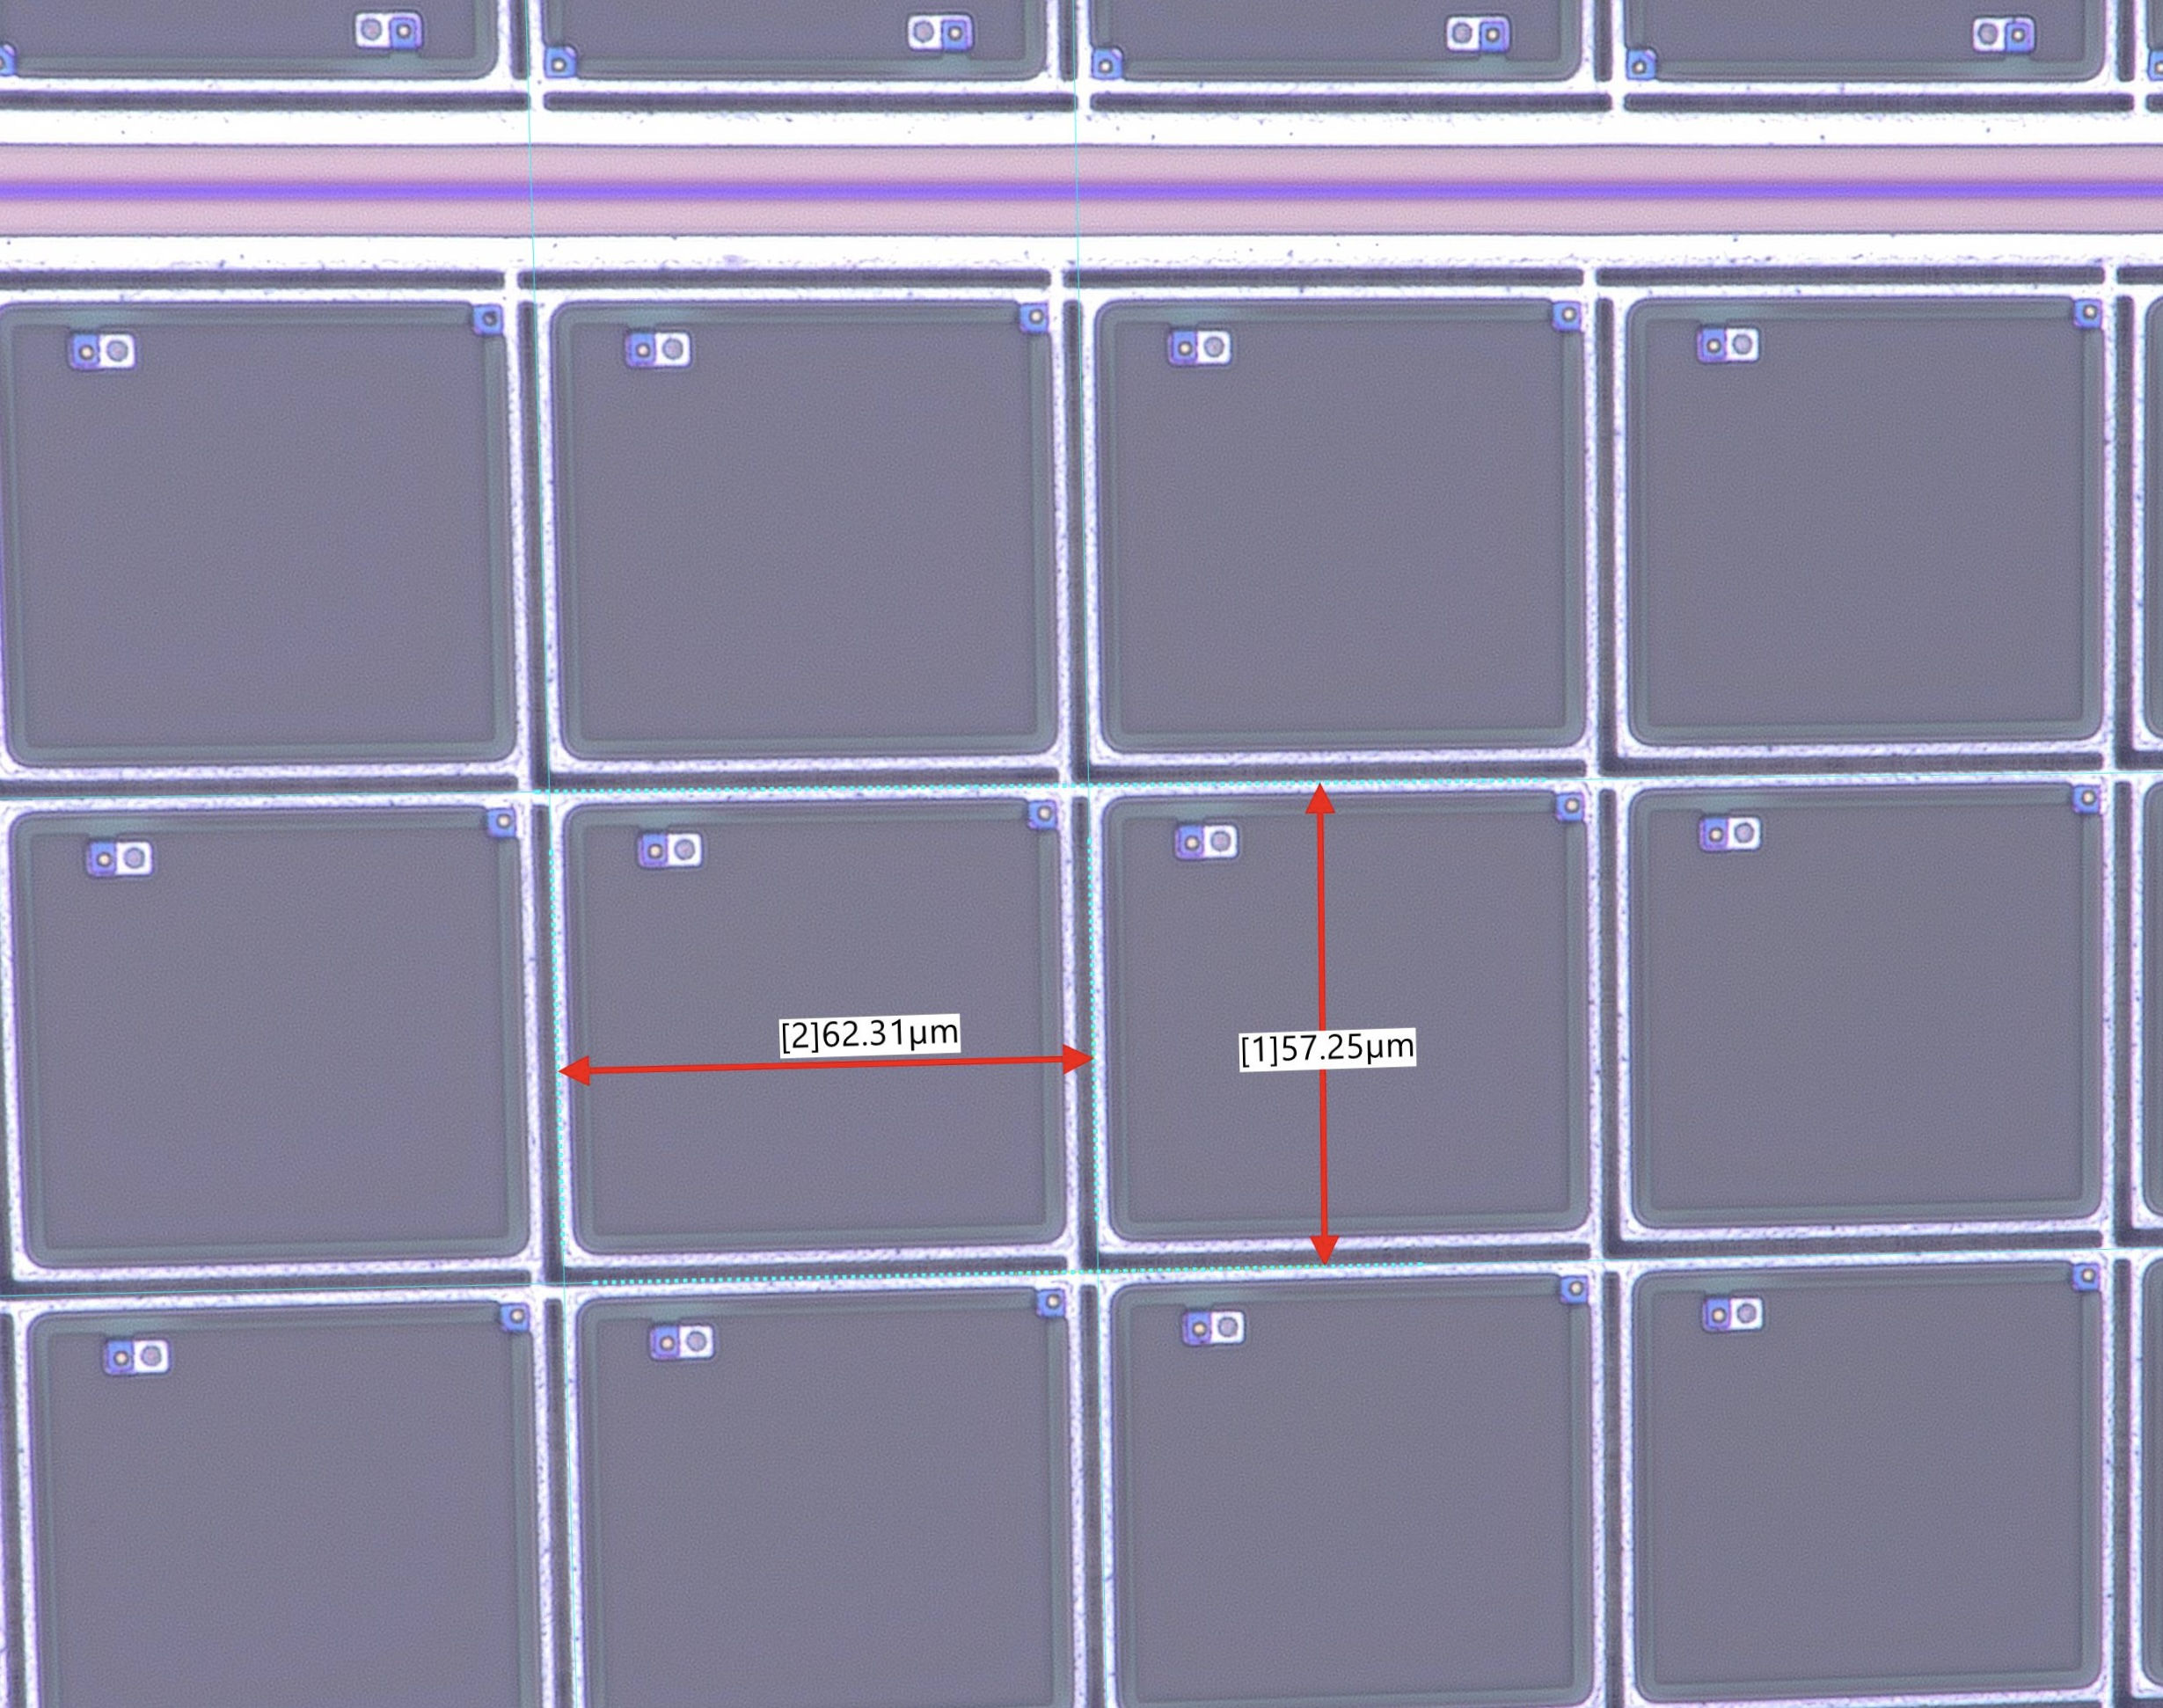
\includegraphics[width=0.8\textwidth]{gfx/pictures/H2017 pixels.jpg}
    \caption{Picture of the H017 detector's pixels with a Keyance optical microscope taken by G. Haefeli. }
    \label{fig:H2017 pixels picture guido}
\end{figure}
%no trenches
%what's it specifity? 





\chapter{Experimental methods}
\label{ch:Experimental setup and methods}
This chapter presents the experimental setups and methods applied to characterise of the FBK and Hamamatsu detectors.

%
% Section: ======================
%
\section{IV curve}
\label{section:IV curve}
The IV characteristic curve represents the measured current of the detector as a function of the bias voltage and can be used to calculate $V_{bd}$ and $R_Q$. Due to the temperature dependency of the quenching resistor, the measurements are performed at constant temperature. This condition in maintained by the activation of an air conditioner in the laboratory. 
Measurements are taken in the light to reduce the signal to noise ratio. 
\subsection{Breakdown voltage} 
The breakdown voltage $V_{bd}$ can be obtained by studying the reverse biased region of the IV curve (where the current shows a steep increase). Several fitting methods to determine $V_{bd}$ where tested
%as explained in \cite{} 
but preliminary results where not as accurate as the method presented in \ref{ch:Experimental methods:breakdown voltage}. 

\subsection{Quenching resistor} 
\label{ch:experiement methods:IV:Rq IV}
The quenching resistance is a key property of a SiPM. In order to measure it, the IV characteristic curve is obtained in the Forward bias operating mode. In this region, the non-linearity of the diode is overcame by the linearity of the quenching resistors ($R_Q$) making the current response proportional to the bias voltage. The slope of this response is used to compute $R_Q$.
The measurement setup is shown in Fig. \ref{fig:pic IV rq setup}. One channel of the SiPM array is connected to a KEITHLEY INSTRUMENTS 2400 source-measure unit with a \SI{50}{\ohm} resistor in series. To avoid any other internal resistors in the electrical circuit, no other apparatus are plugged. 
\begin{figure}[htbp]
    \centering
    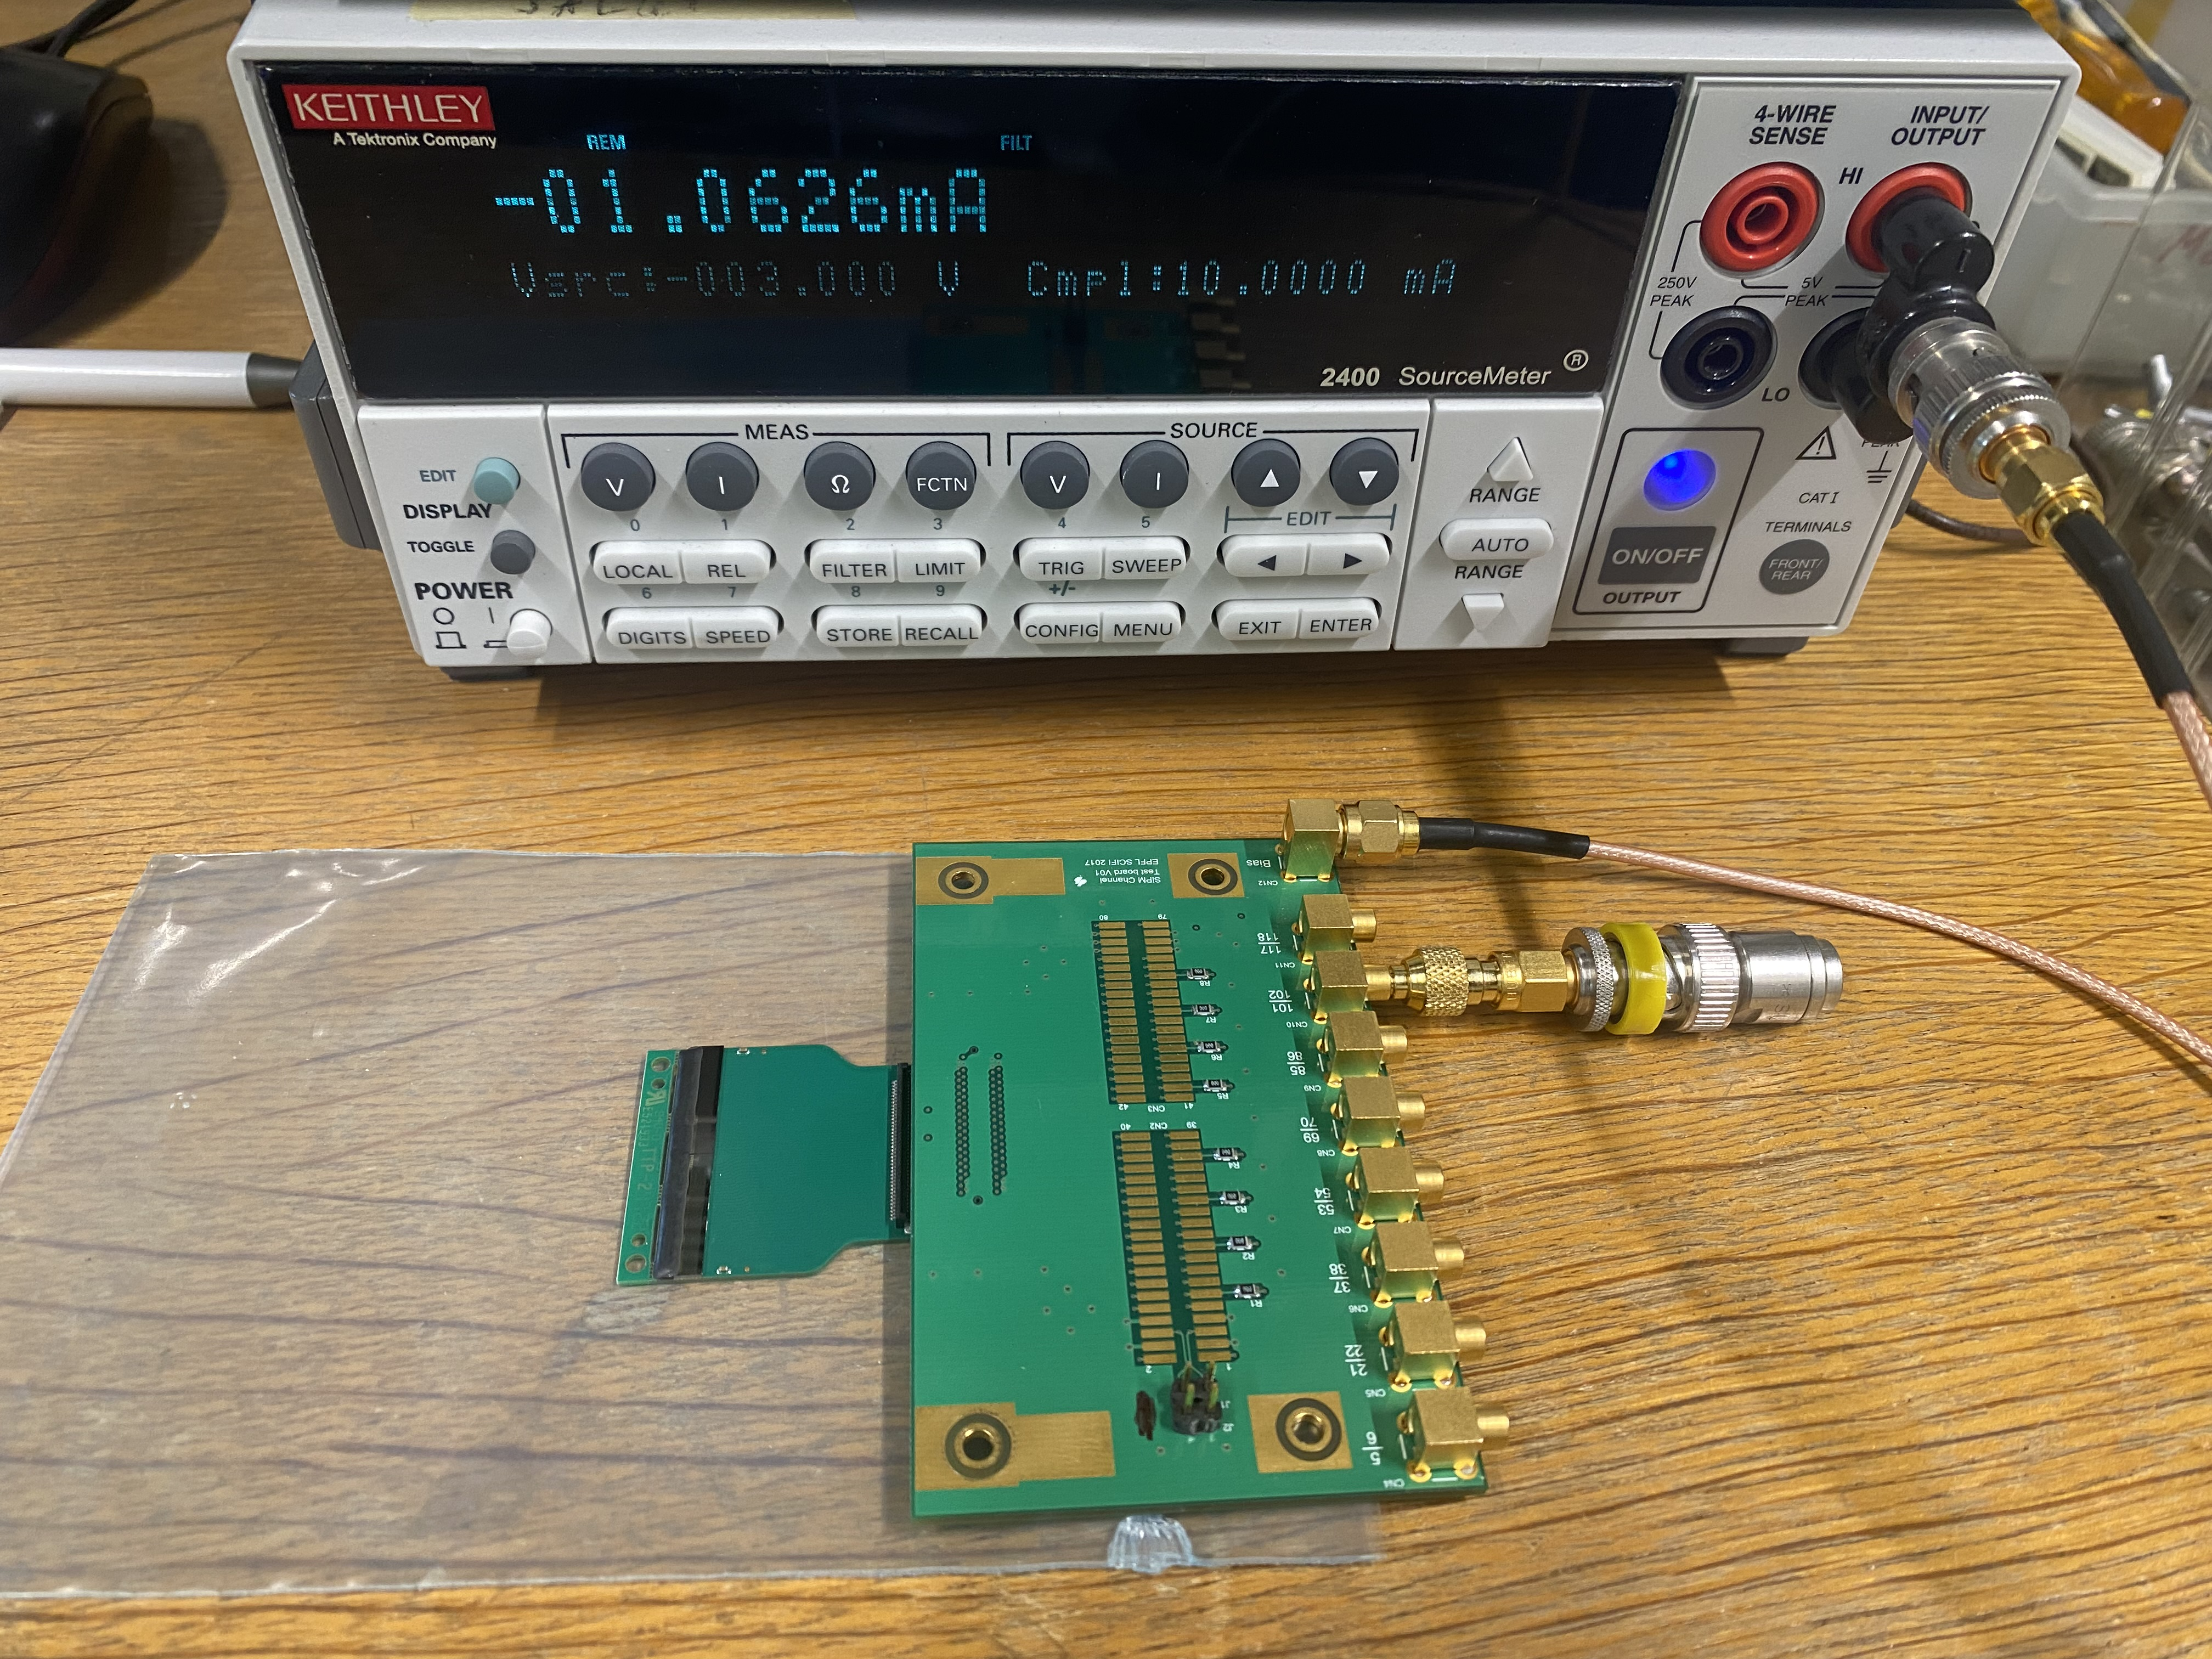
\includegraphics[width=0.8\textwidth]{gfx/pictures/Rq_IV_setup.png}
    \caption{Picture of the experimental setup for the measurement of $R_Q$ with the IV-curve method.}
    \label{fig:pic IV rq setup}
\end{figure}
The SiPM array is connected to a \ac{PCB} where only 8 outputs are available. Theses PCBs allow to characterize 16 channels, 8 ODD and 8 EVEN \footnote{channels analysed: $[5,6, 21,22, 37,38, 53,54, 69,70, 85,85, 101, 102, 117, 118]$}, and minimize the serial resistances from electrical wires. The photo-current coming from the SiPM is measured at different bias voltages in the forward bias region. 
A python script performs the measurement by taking the data from the instrument. An averaging of $10$ current values is taken to counter the influence of noise. 
With this method, the IV characteristics is obtained. The quenching resistance is inversely proportional to the slope of the linear region in the IV curve. In absence of external resistors,  Eq. \eqref{eq:original quenching resistor1} applies:
\begin{equation*}
  \begin{minipage}[t]{0.48\linewidth}
        \begin{equation}
            R_Q = N_{pixels}\cdot \left(\frac{dV}{dI}\right)
        \label{eq:original quenching resistor1}
        \end{equation}
  \end{minipage}
  \hfill
  \begin{minipage}[t]{0.48\linewidth}
        \begin{equation}
            R_Q = N_{pixels}\cdot \left(\frac{dV}{dI} - \SI{50}{\ohm} \right)
        \label{eq:original quenching resistor}
        \end{equation}
  \end{minipage}  
\end{equation*}

Taking into account the resistor of \SI{50}{\ohm} plugged in series to the circuit, the formula becomes Eq. \eqref{eq:original quenching resistor}.
Note that $N_{pixels}$ is the number of pixels contained in one channel for a detector. 
\\
This method is strongly dependent on the choice of the fitting range. Going too high in $V_{bias}$ heats the detectors and changes the value of $R_Q$. On the other hand going too low, the IV curve's behavior is not linear anymore (diode response not negligible). The fitting range has been discussed with the manufacturer to have consistency in the methods \cite{StefanoMerzi2023PrivateCommunication}. For the H2017, the fitting range is the same as in \cite{Girard2018CharacterisationDistributions}. Results are shown in Section \ref{ch:Results:Rq}.

\paragraph{uncertainties.} The statistical uncertainties are negligible due to the goodness of the linear fit. 
Channel to channel, a variation of $5\%$ in the quenching resistor values is observed. The connection between the channel to the IV setup introduce serial resistances order of magnitude of \SI{1}{\ohm}. This error is bigger on the \SI{16}{\micro m} since it has the larger number of pixel $\approx 1\%$ whereas $0.1\%$ for the \SI{31}{\micro m}. The total uncertainties is then $\pm 6\%$ for the \SI{16}{\micro m} and $\pm 5\%$ for the other detectors. 
The results are presented in section \ref{ch:Results:Rq}.


\section{Waveform analysis}
\label{section:waveform analysis}

\begin{figure}[http]
    \centering
    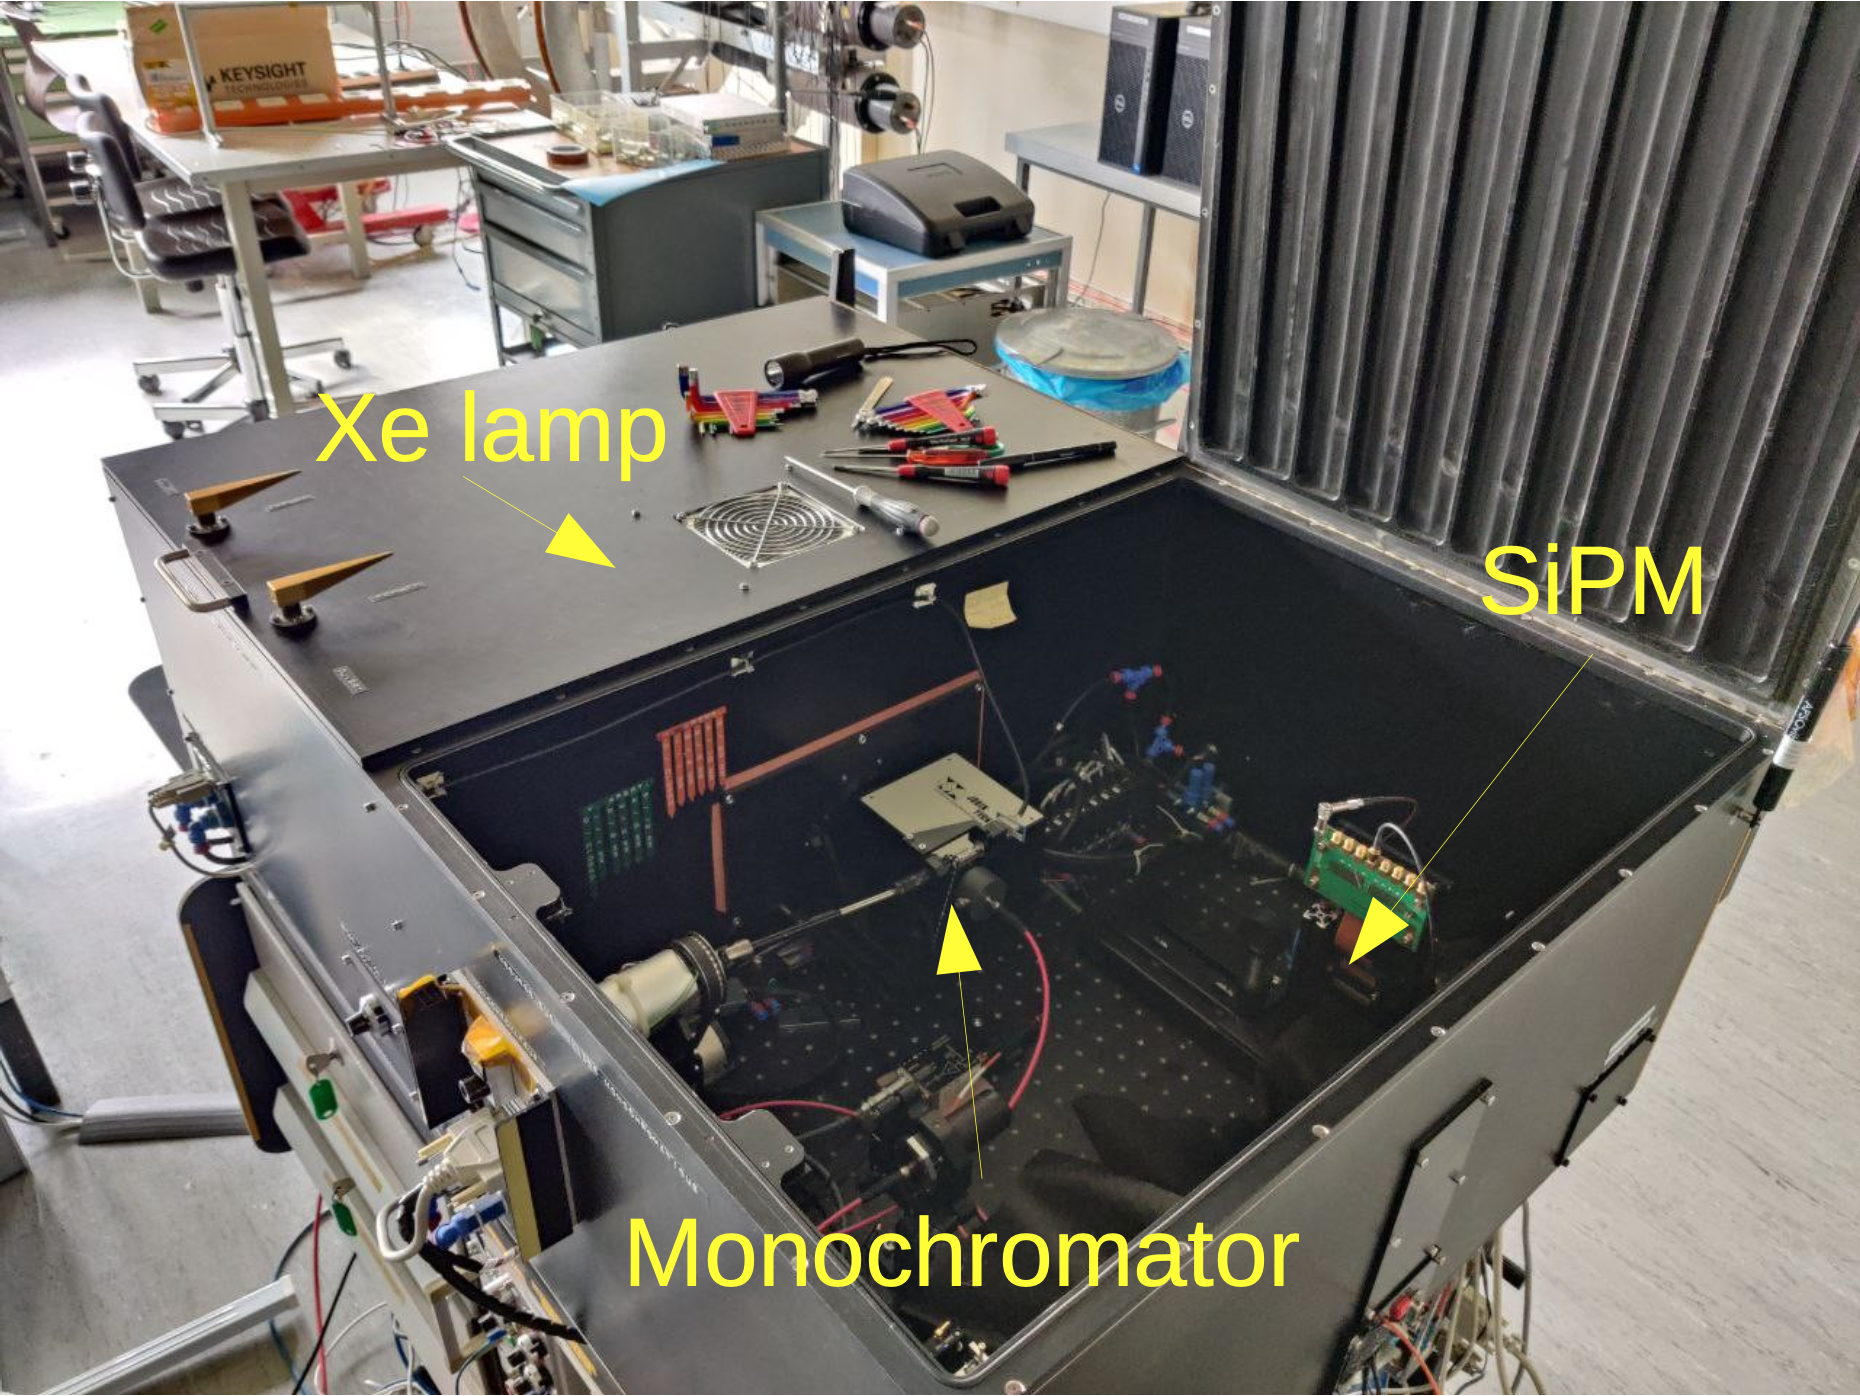
\includegraphics[width=0.8\textwidth]{gfx/pictures/PDE_setup.png}
    \caption{Photograph of the waveform analysis and PDE measurement setup.}
    \label{fig:PDE setup pic}
\end{figure}
Recording the waveforms produced by the detectors allow to measure several characteristics. 
\subsection{Setup}
\label{ch:Experimental setup:WA:setup}
The detector is in a black box shown in Fig. \ref{fig:PDE setup pic} that shields electromagnetic interference to limit the electronic noise\footnote{The Xe light is not used yet (see \ref{ch:Experimental methods:Gain and PDE:setup})}. The detector is mounted on a PCB, connected to a bias voltage\footnote{KEITHLEY INSTRUMENTS 2400},the signal is amplified (\SI{40}{dB}) and connected to the oscilloscope. A picture showing the connection of the channel to the PCB is shown in Fig. \ref{fig:PCB channel picture}:
\begin{figure}[htbp]
    \centering
    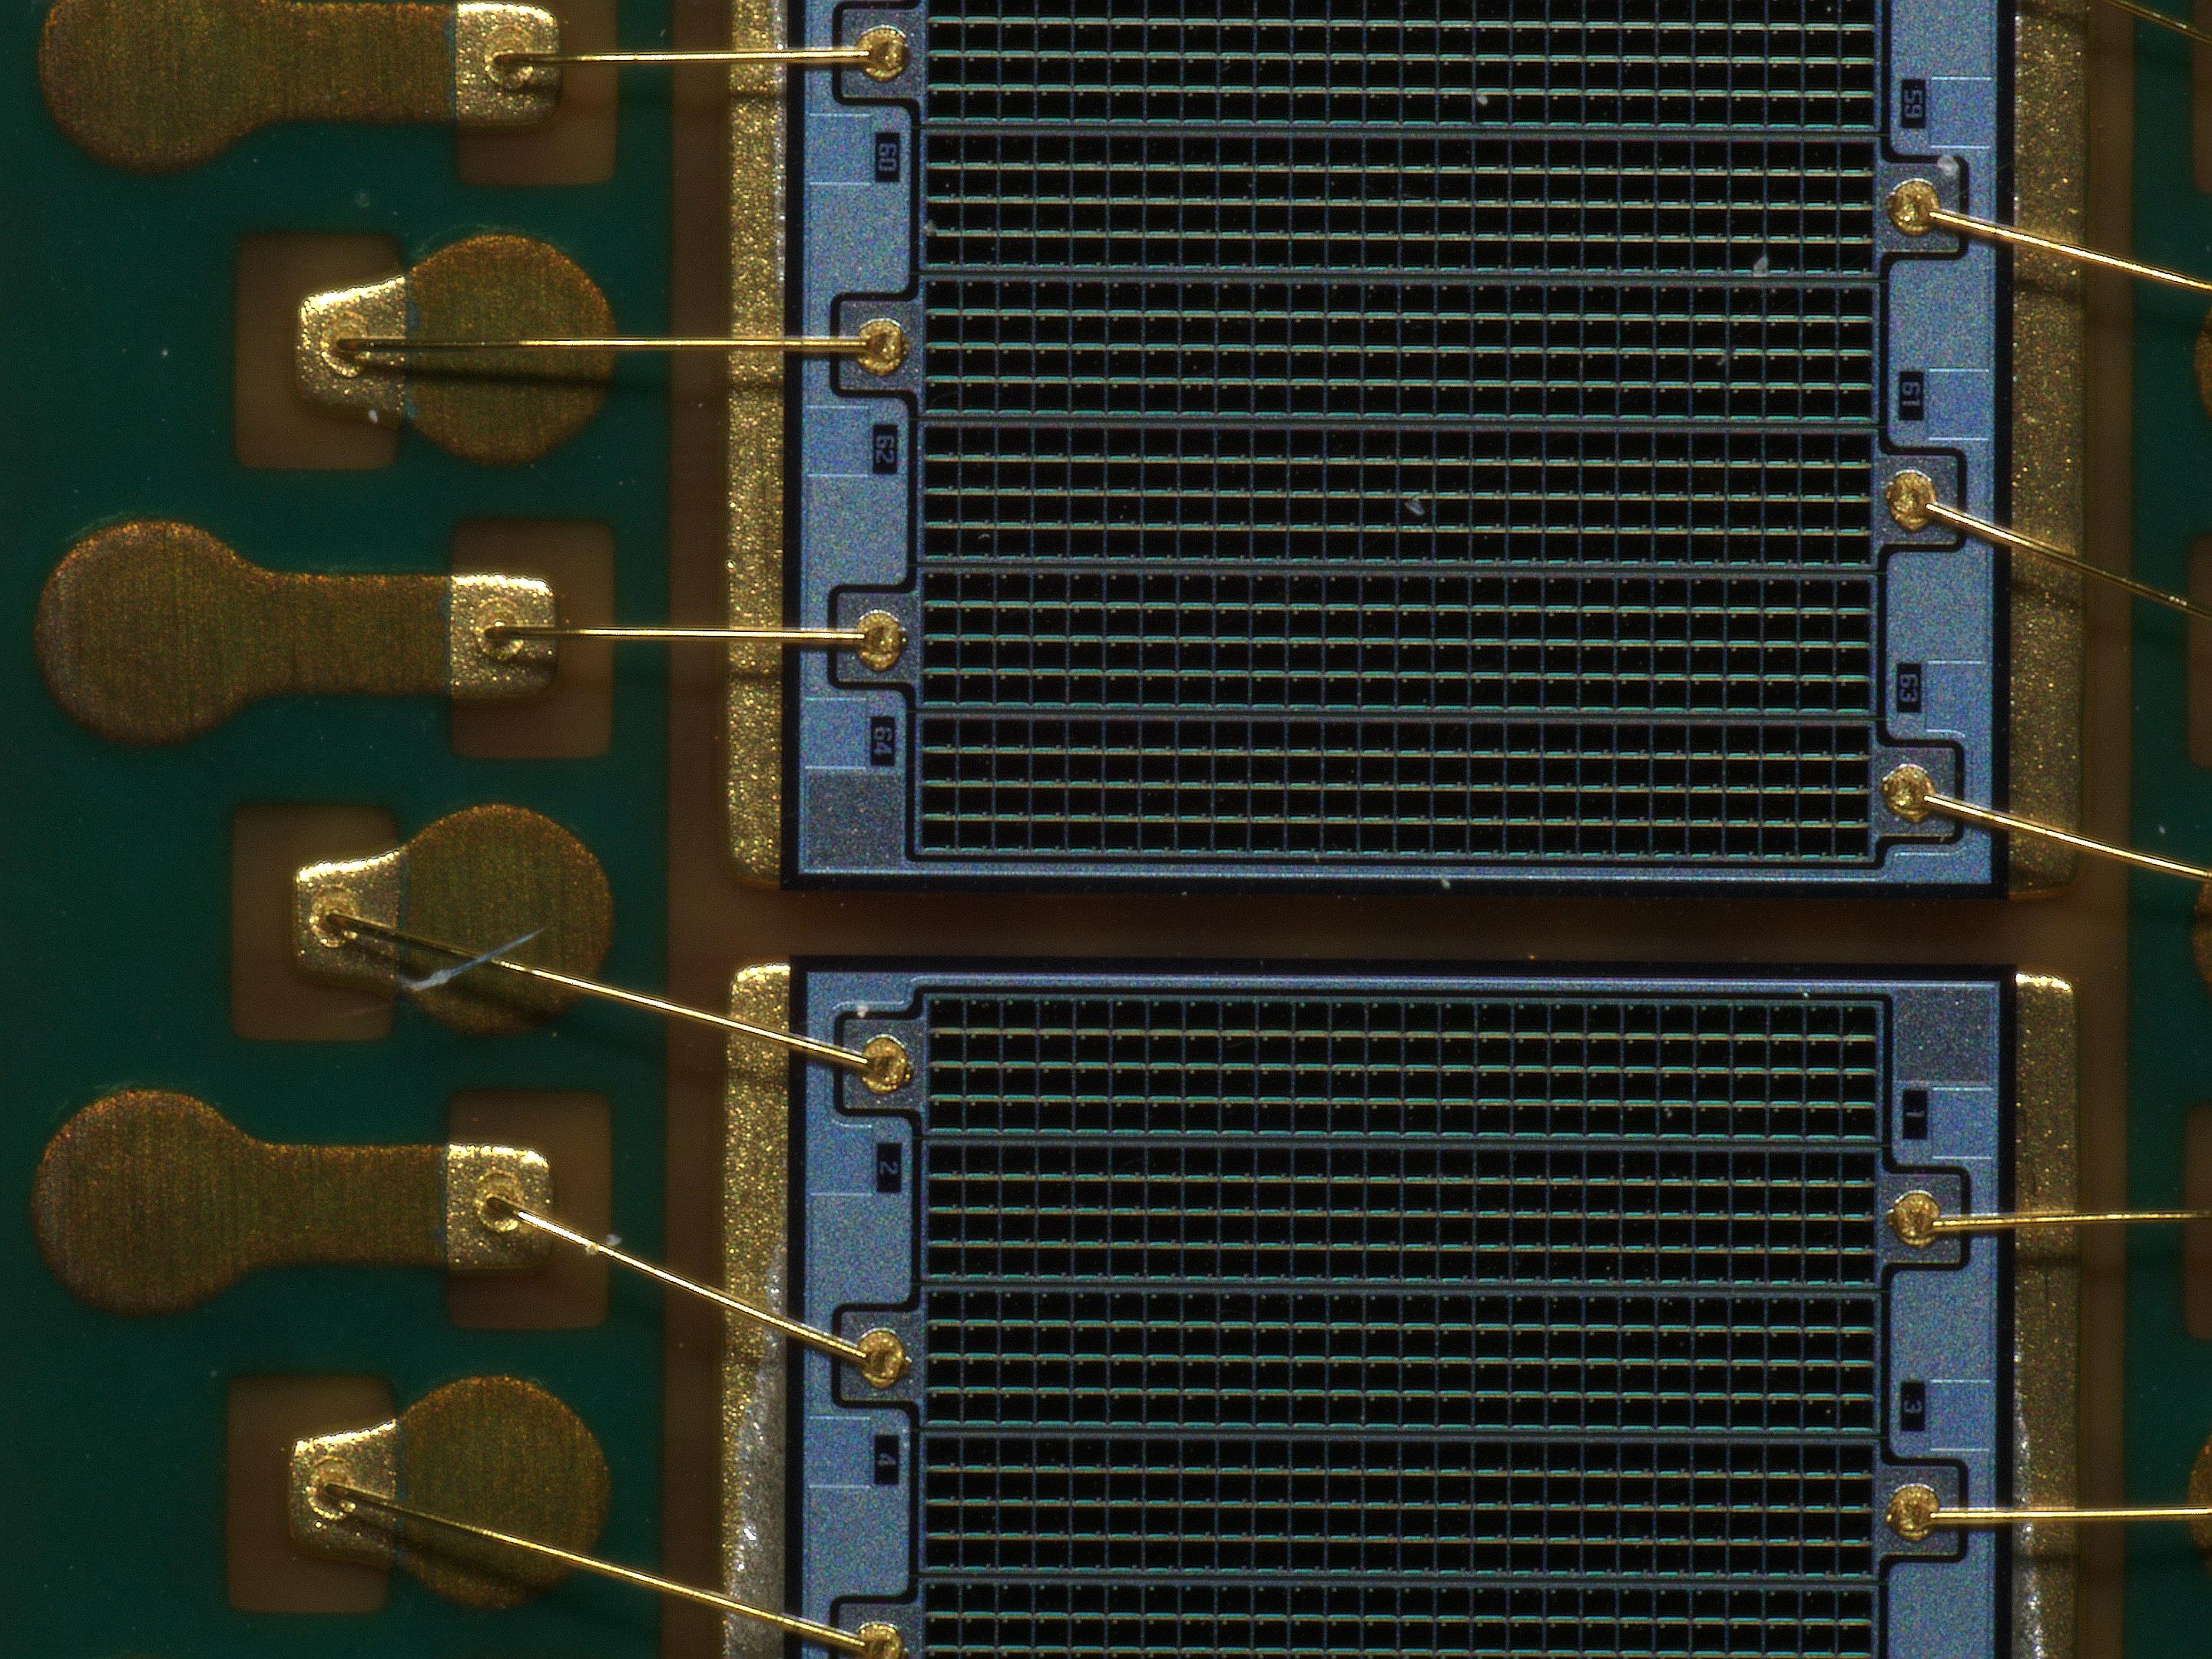
\includegraphics[width=0.8\textwidth]{gfx/pictures/PCBchannel.jpg}
    \caption{H2017 channel bonding to the PCB. Picture taken by G. Haefeli with a Keyence microscope. }
    \label{fig:PCB channel picture}
\end{figure}
A black cloth is wrapped around the detector so that only waveforms corresponding to noise are recorded.
The oscilloscope records the waveforms triggered on a $1$ PE signal, meaning on a dark count. The single photons waveforms are defined as clean waveforms. By doing this, the correlated noise such as DiXT, DeXT and AP are identified on the waveforms with a software. It is important to tune the thresholds for different types of noise, so that the script identifies and classify the waveforms accordingly. The breakdown voltage $V_{bd}$ is also measured by recording the waveforms in this configuration. The measurement are taken at fixed temperature of \SI{25.0}{\celsius} to avoid the temperature dependency of $V_{bd}$ and the correlated noise. A PT100 temperature sensor is connected to the PCB to know the temperatures during the measurement. 

\subsection{Breakdown Voltage}
\label{ch:Experimental methods:breakdown voltage}
By measuring the mean peak amplitude of $1$ PE pulses, such as the one shown in Fig. \ref{fig:mean pulse amplitude}, the breakdown voltage is obtained. 
The relation between the pulse amplitude and overvoltage is linear, therefore the dependency can be fitted and the extrapolation to zero is the breakdown voltage. This method has proven to be really effective and trust full, allowing to reach a level of precision by the order or \SI{200}{\milli V}.


\paragraph{uncertainties.}  The systematic uncertainties are estimated\footnote{Evaluated with different measurements, with different $V_{bias}$ ranges.} to be $\pm$ \SI{200}{\milli V}. Due its lower signal to noise ratio, the systematics uncertainties as expected to be higher for the FBK \SI{16}{\micro m} with $\pm$ \SI{300}{mV}.
The statistical uncertainties are of the order of \SI{10}{ \milli V}, so negligible compared to the systematics.
The results are presented in section \ref{ch:Results:breakdown voltage}.


\begin{figure}[htbp]
  \centering

  \begin{subfigure}{0.48\textwidth}
    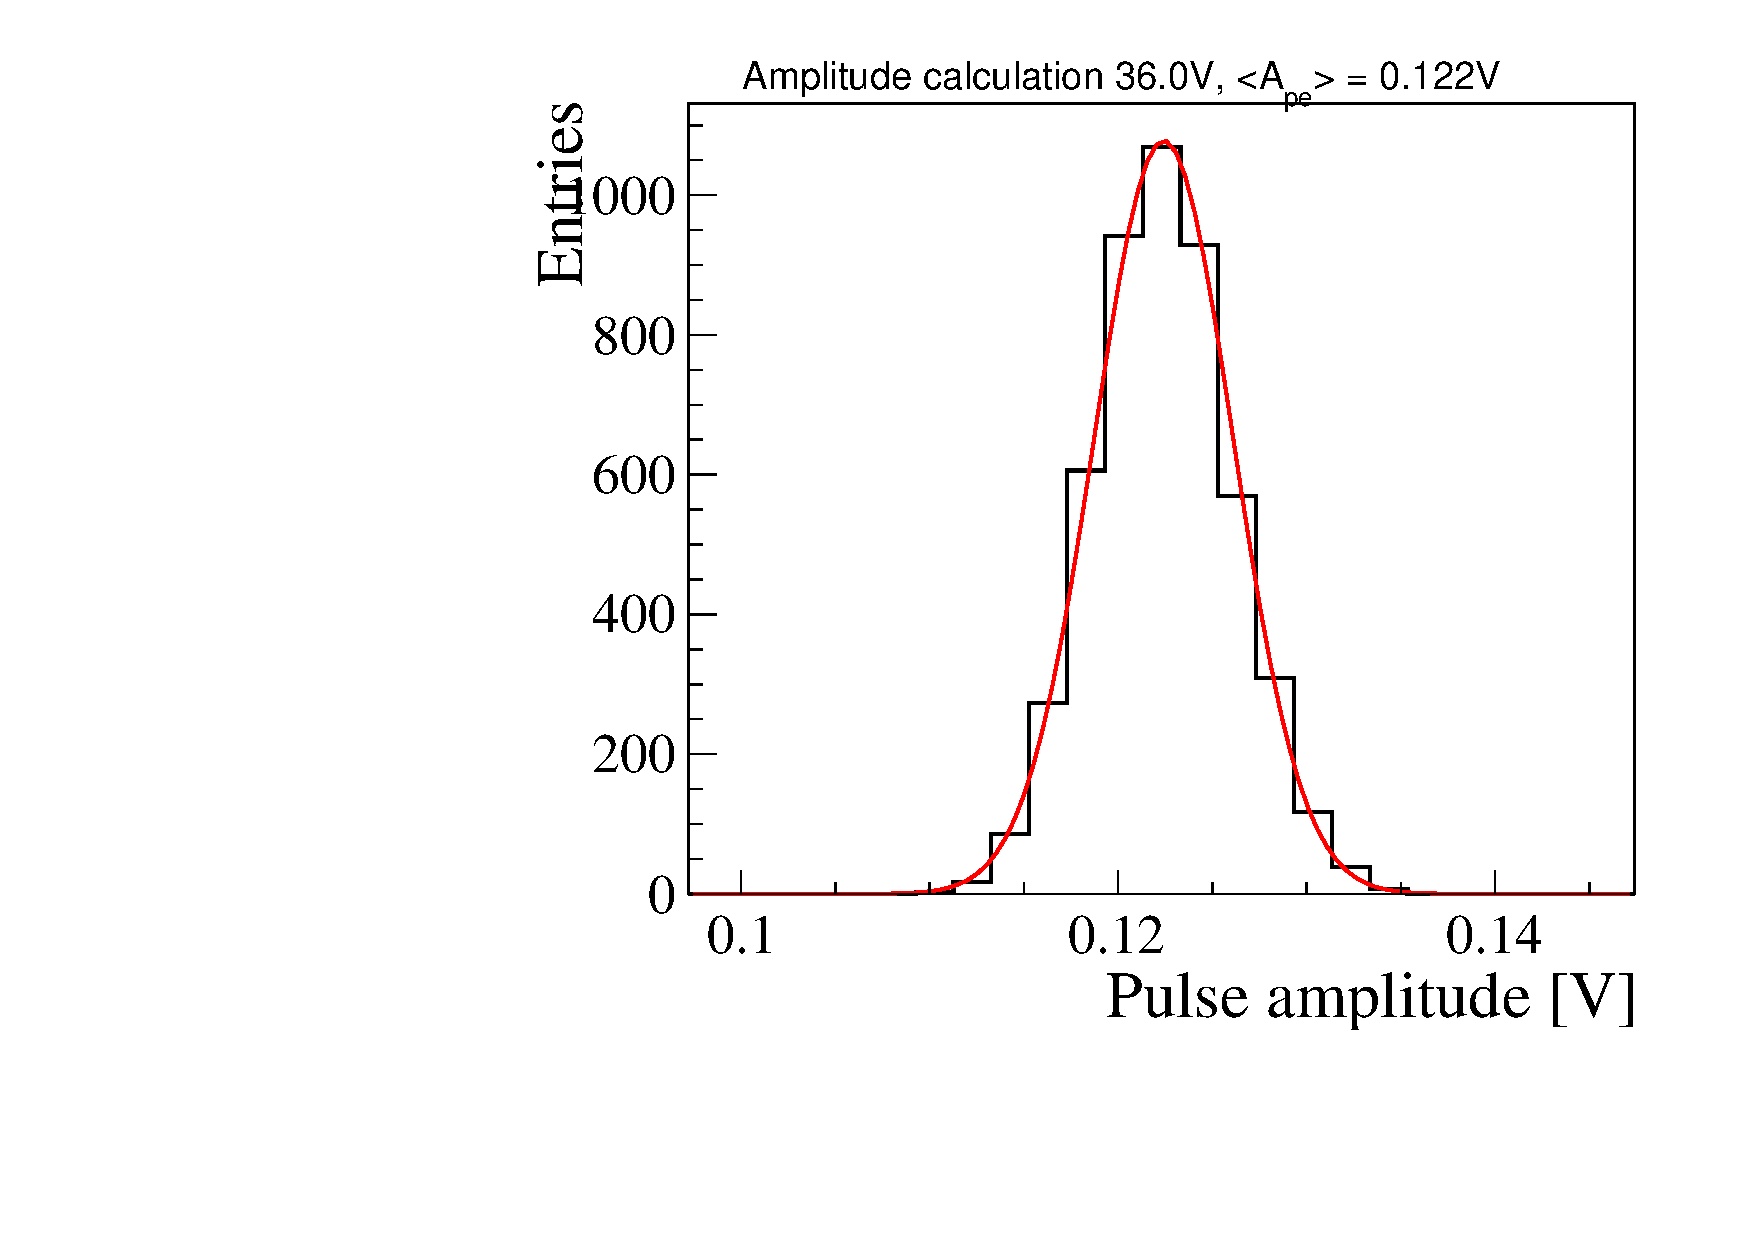
\includegraphics[width=\textwidth]{gfx/plots/examples/peakamp_36V_FBK31.pdf}
    \caption{}
  \end{subfigure}
  \hfill
  \begin{subfigure}{0.48\textwidth}
    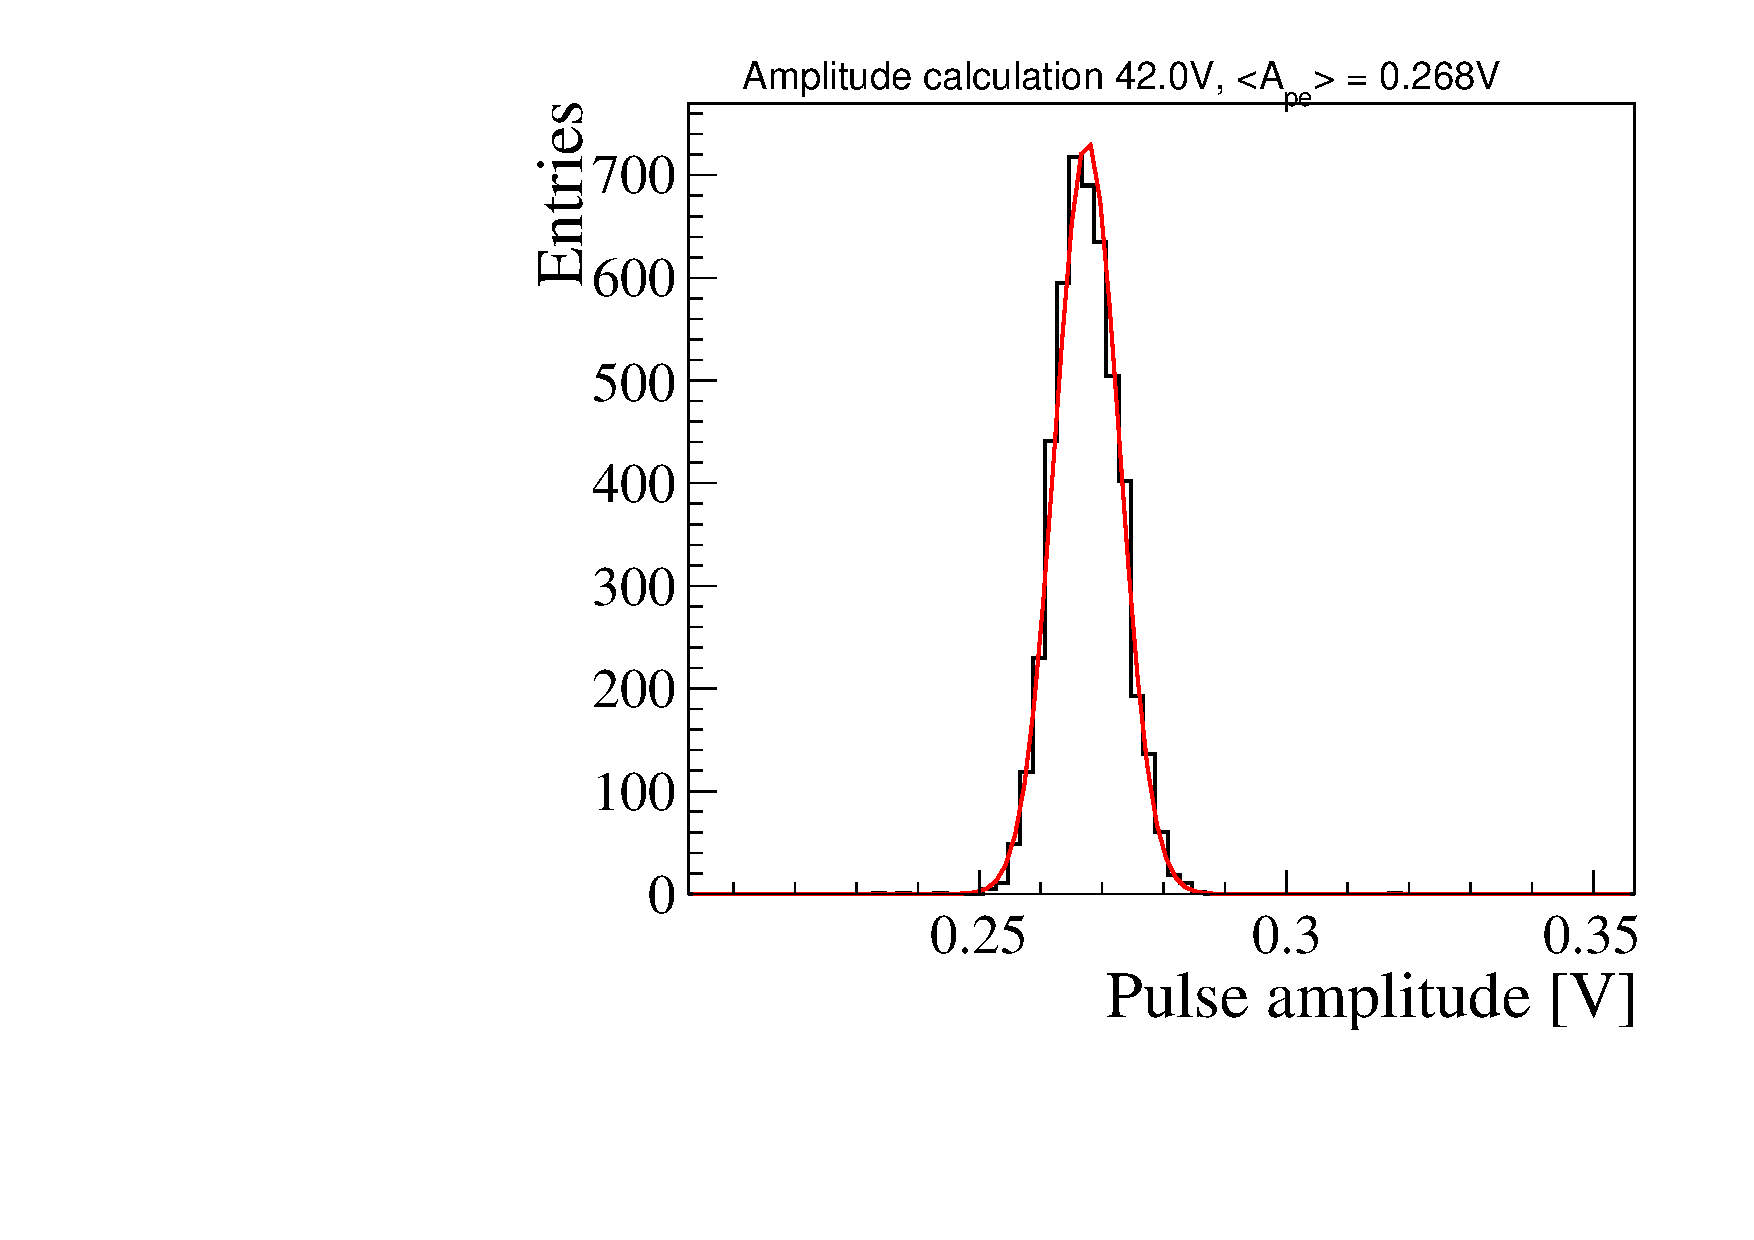
\includegraphics[width=\textwidth]{gfx/plots/examples/peakamp_42V_FBK31.pdf}
    \caption{}
  \end{subfigure}
  
  \caption{Mean peak amplitude for the SiPM FBK \SI{31}{\micro m}, channel $22$ at $5$V (a) and $11$V (b) overvoltage.}
  \label{fig:mean pulse amplitude}
\end{figure}
 


\subsection{Noise classification}
\label{ch:Experimental methods:Noise identification}
As introduced above, the waveforms are recorded by the oscilloscope and then analysed in the software. For these measurement, the temperature is fixed at \SI{25.0}{\celsius} and $5000$ waveforms are stored for each overvoltage values.

The waveform analysis software for the correlated noise is included in the determination of the breakdown voltage. To distinguish the different noises, thresholds on the time and amplitude of the waveforms need to be given as inputs. These thresholds are dependant on the SiPM pulse shape and are adapted by analysing the waveforms. This depends on the detector's features such as the value of $R_Q$ or the pixel size, etc and leads to different pulse shapes. On Fig \ref{fig:clean waveform comparison}, the difference is the pulse shape of a $1$ \ac{PE} clean signal is clearly visible. On the FBK, a plateau is present whereas on the H2017, the pulse goes to the baseline way much faster. 
\begin{figure}[htbp]
  \centering

  \begin{subfigure}{0.48\textwidth}
    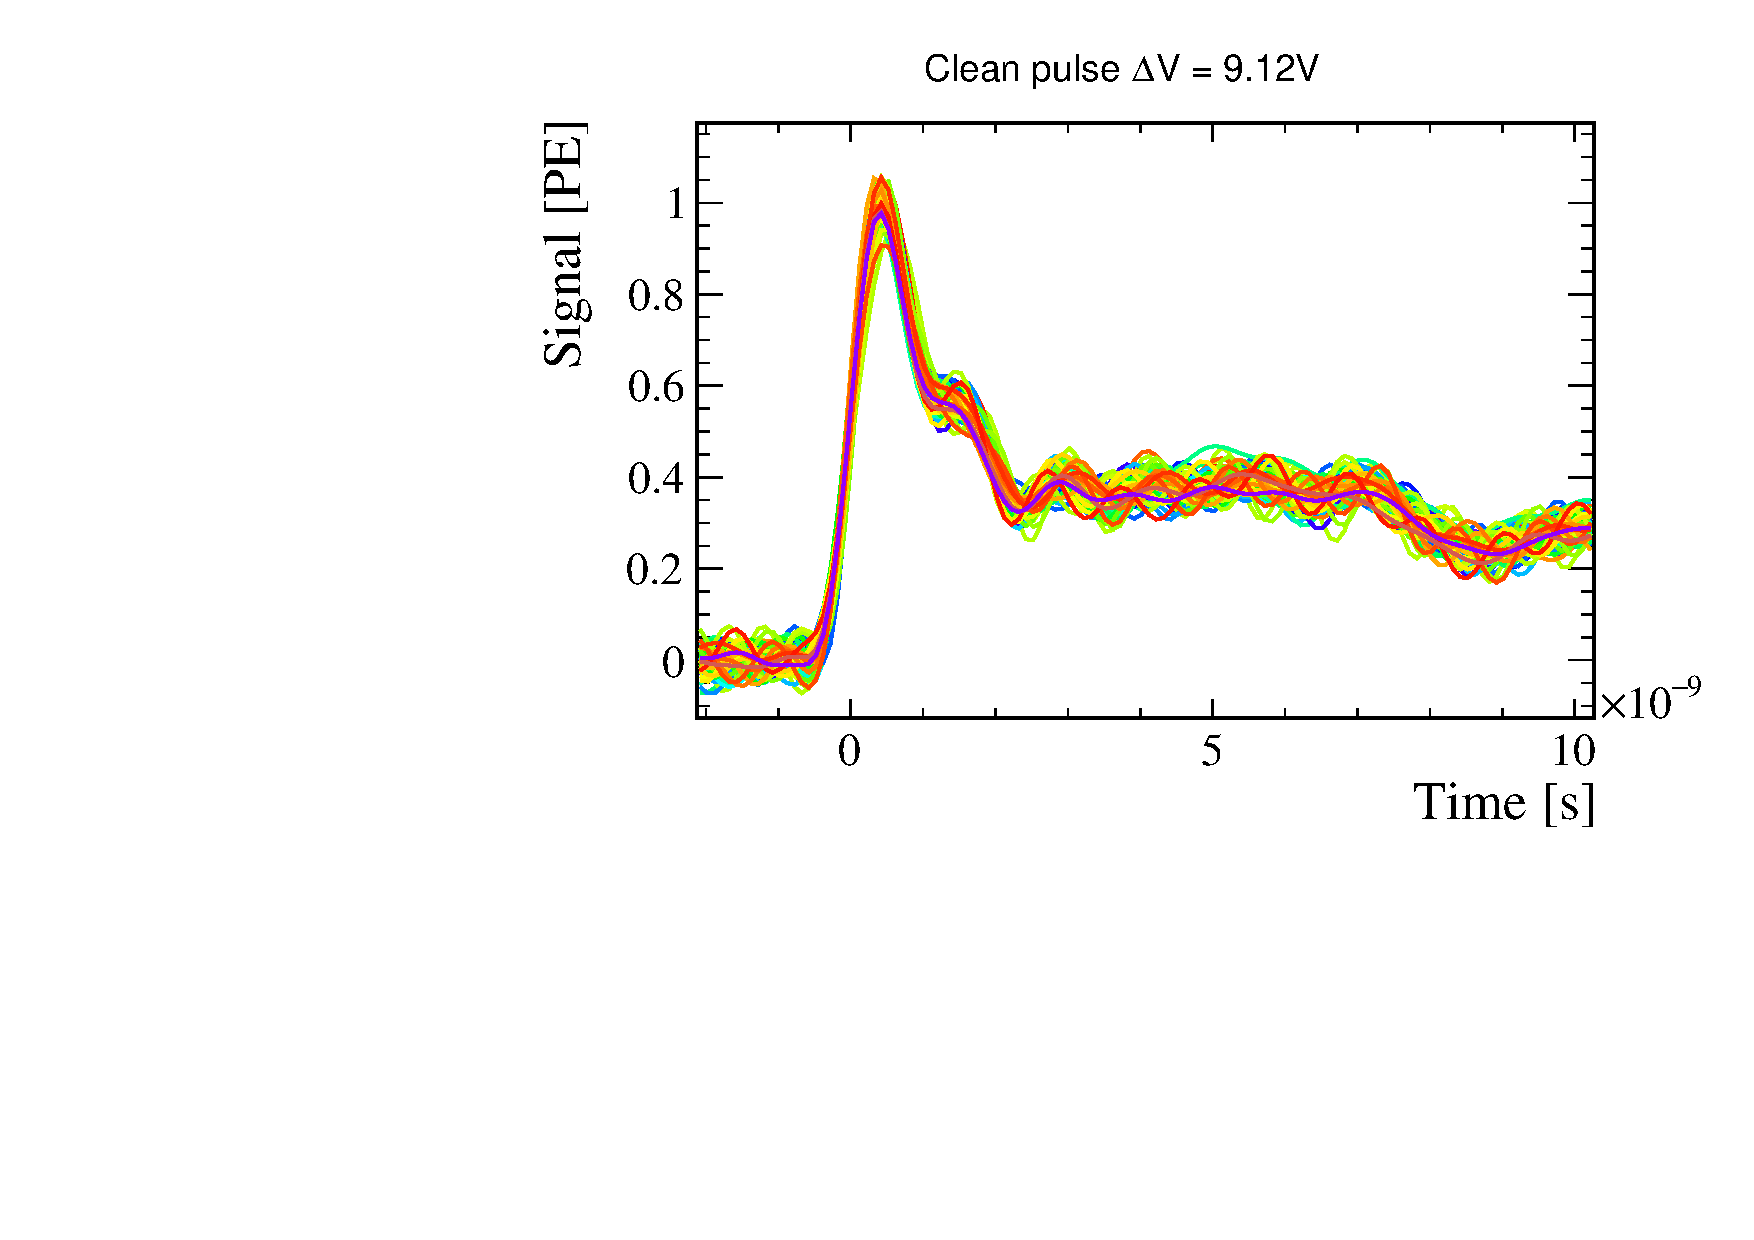
\includegraphics[width=\textwidth]{gfx/plots/WA/31/clean_10ns.pdf}
    \caption{}
    \label{fig:31/clean_10ns}
  \end{subfigure}
  \hfill
  \begin{subfigure}{0.48\textwidth}
    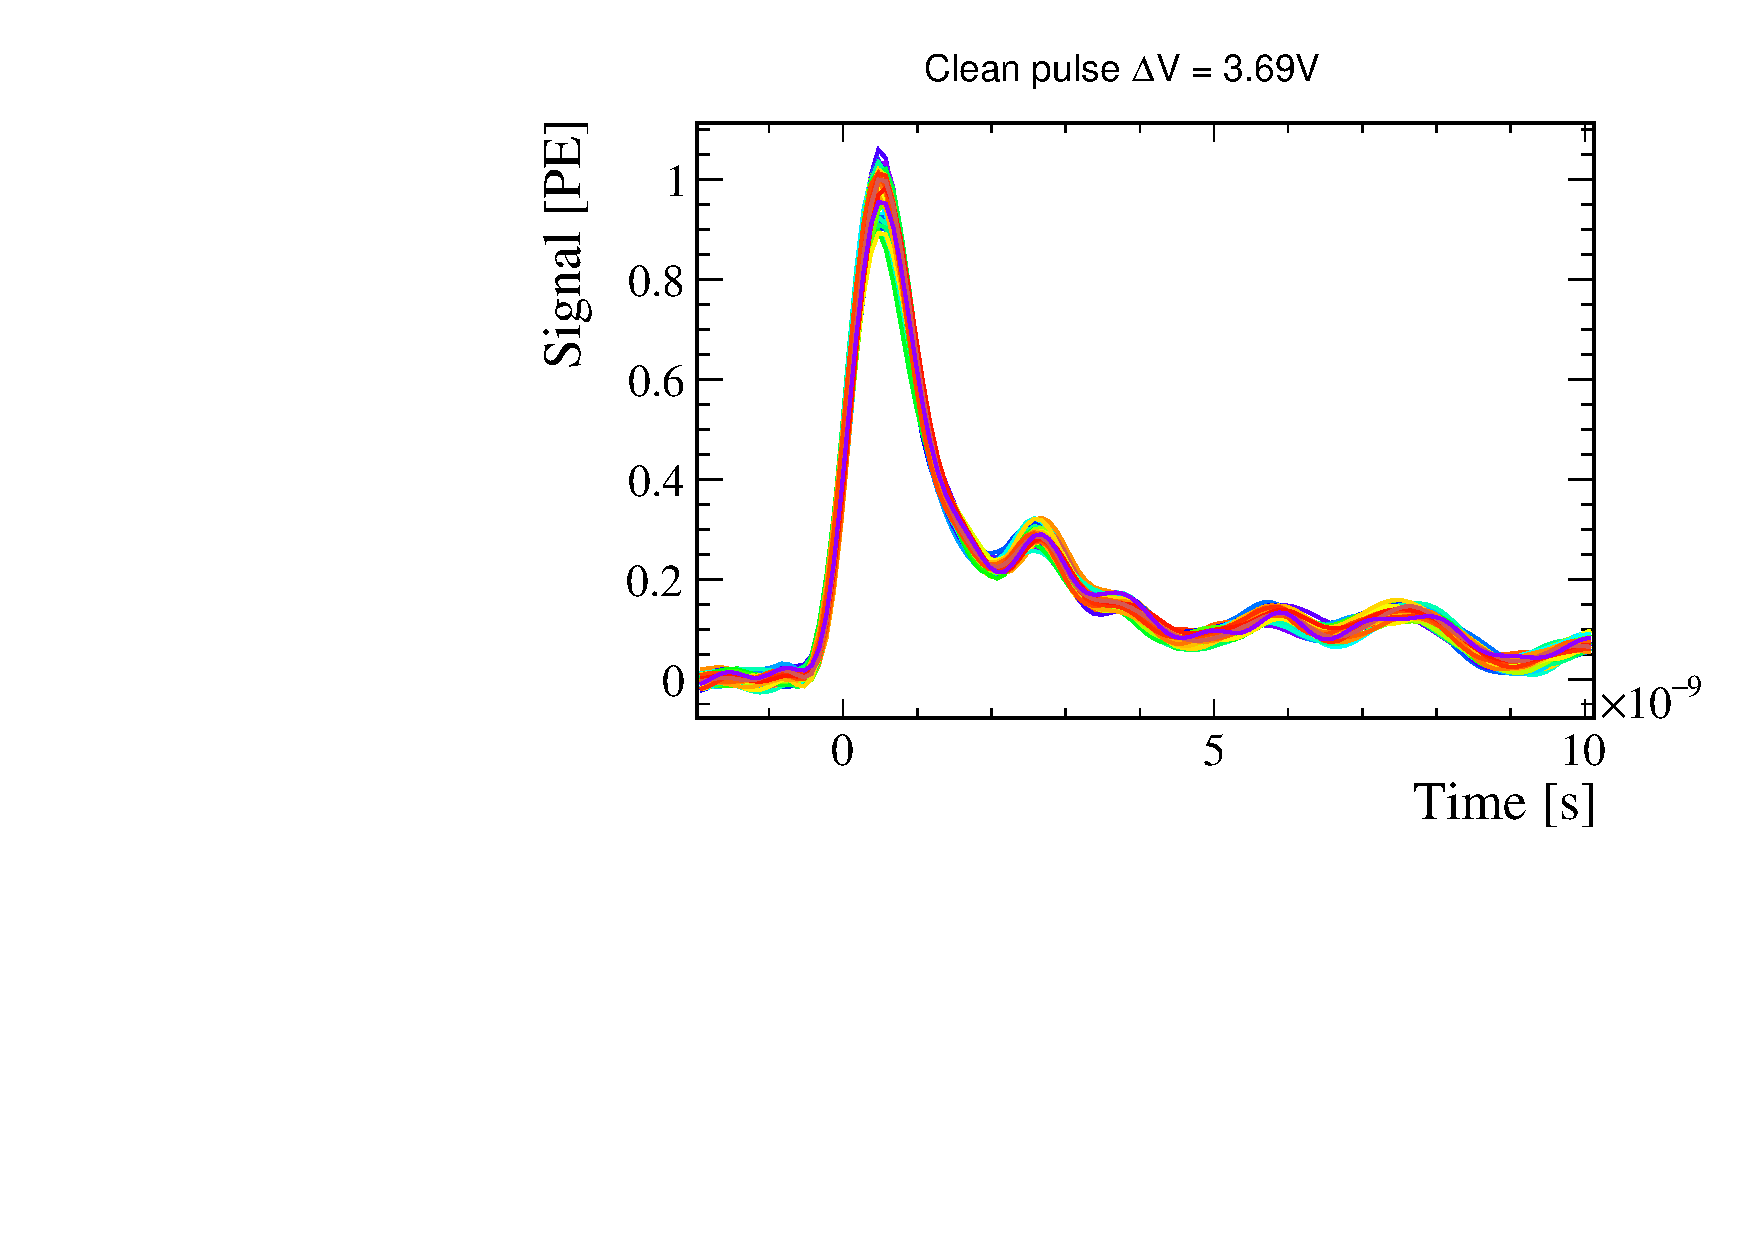
\includegraphics[width=\textwidth]{gfx/plots/WA/H2017/clean_10ns.pdf}
    \caption{}
    \label{fig:H2017/clean_10ns}
  \end{subfigure}
  \caption{FBK \SI{31}{\micro m} detector  and Hamamatsu H2017  clean waveform comparison.}
  \label{fig:clean waveform comparison}
\end{figure}

Fig. \ref{fig: mix waveforms and thresholds} shows a plot of the different waveforms for a fixed overvoltage. One can see the classification of the different correlated noises for the FBK \SI{31}{\micro m} detector. 
The results of the noise classification are presented in section \ref{ch:Results:Noise Classification}.

\begin{figure}[htbp]
  \centering
    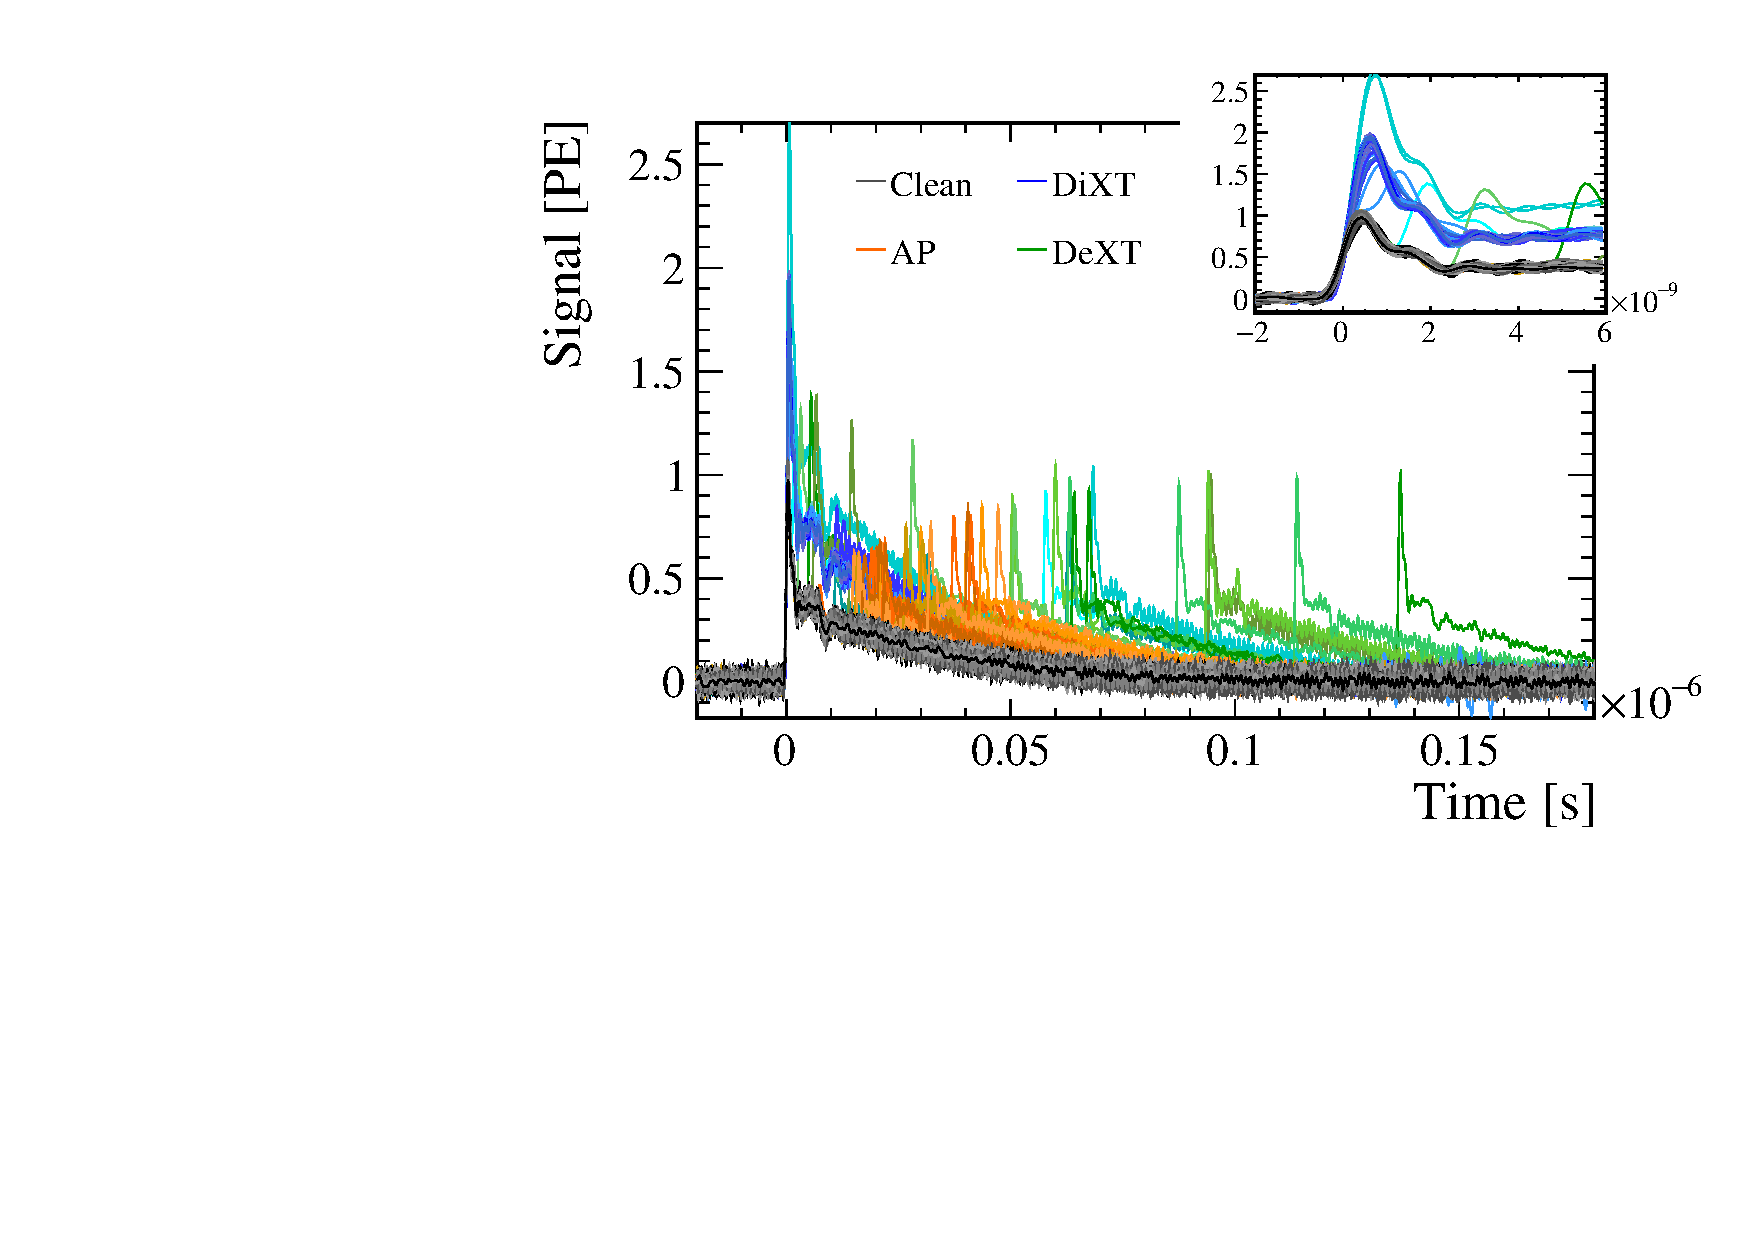
\includegraphics[width=\textwidth]{gfx/plots/WA/31/mix.pdf}
    \caption{After the analysis, different correlated noises waveforms classified (for FBK \SI{31}{\micro m} detector).}
     \label{fig: mix waveforms and thresholds}
\end{figure}


% =========== WA =========== %

% ========== PDE ==========  %



% alternative organisation



\subsection{Quenching resistor} 
\label{ch:experiement methods:WA:Rq WA}
The quenching resistor can be obtained from the waveform analysis by measuring the time constant $\tau_{long}$, which represents the slow component of the pulse shape. It is obtained by fitting the clean pulse of $1$PE as Fig. \ref{fig:taulong fit} shows. The average clean waveforms are displayed in log scale and a linear fit is applied to get the $\tau_{long}$ value. 
\begin{figure}[hbtp]
    \centering
  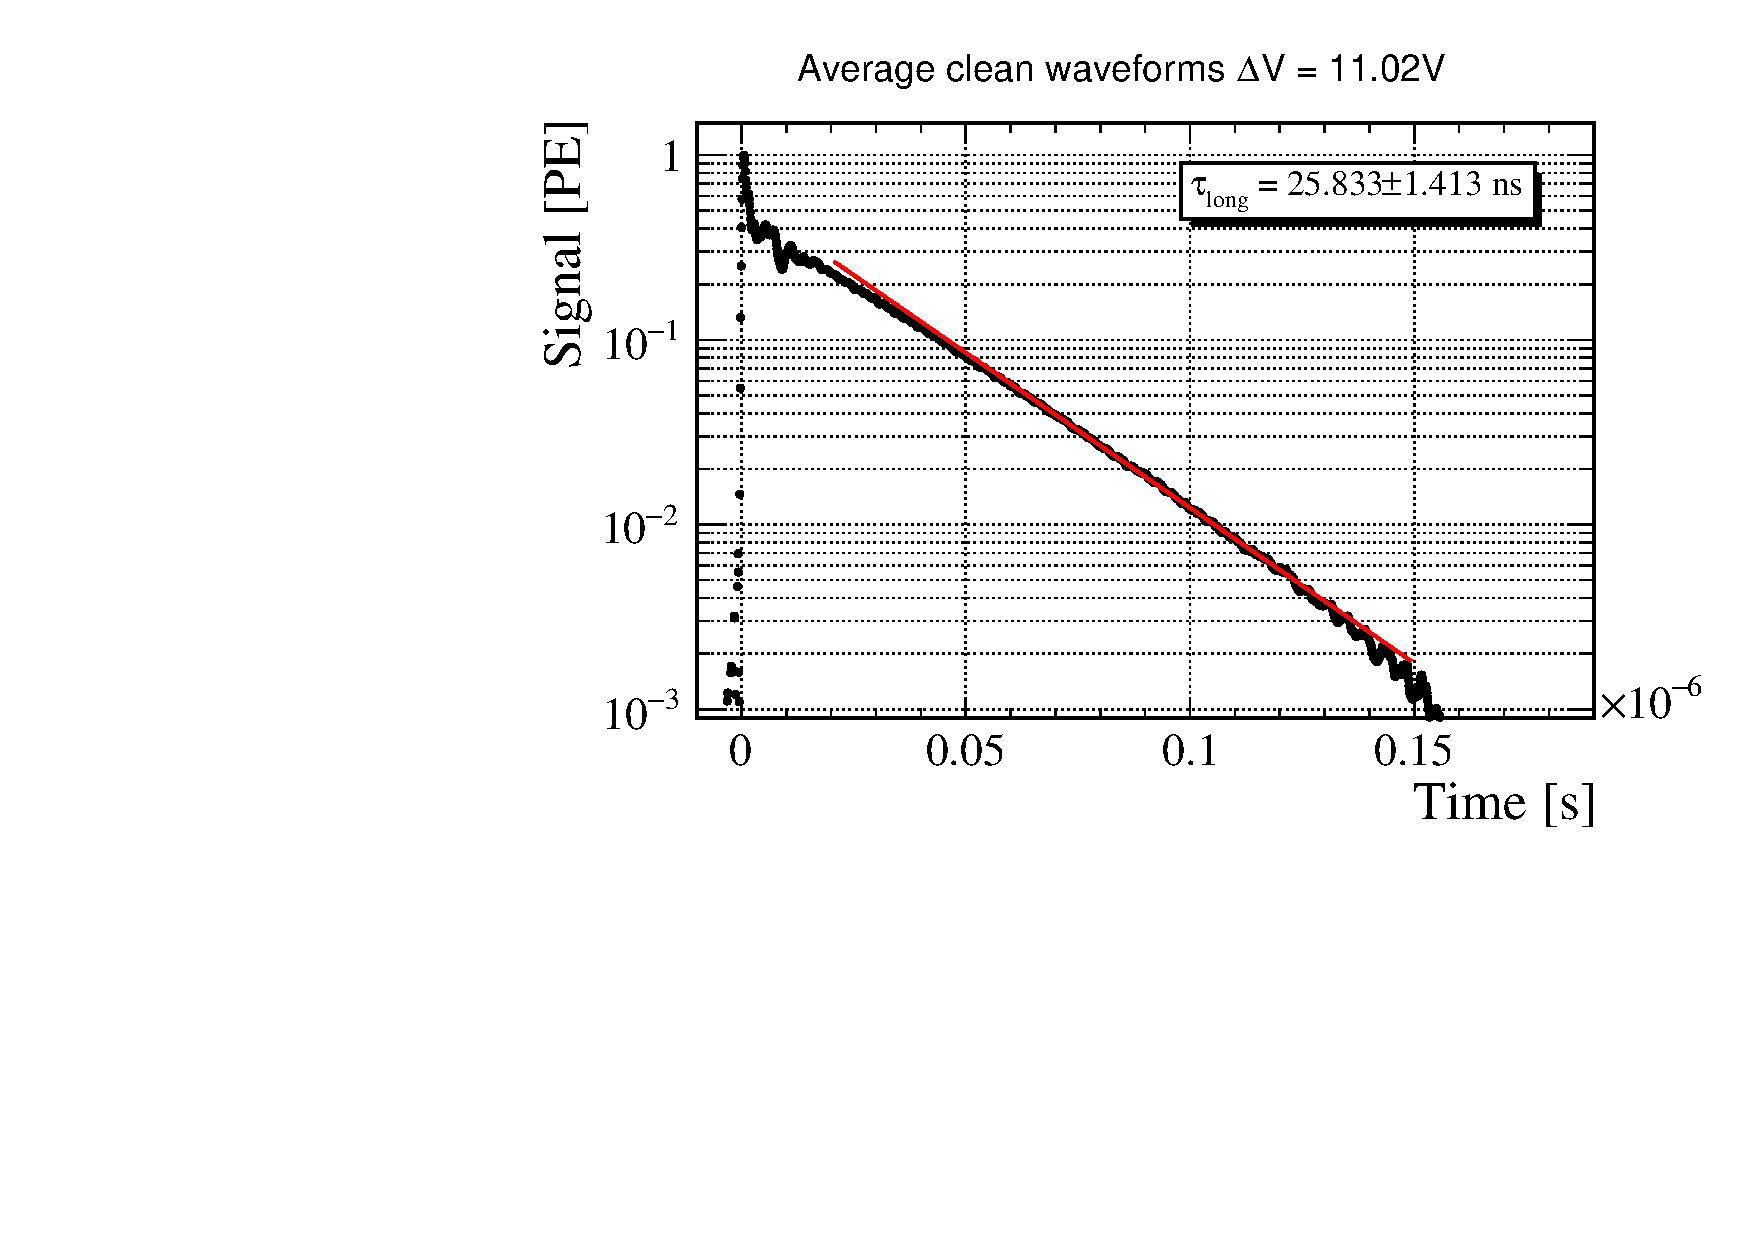
\includegraphics[width=0.7\textwidth]{gfx/plots/WA/31/taulong.pdf}
    \caption{$\tau_{long}$ determination for one overvoltage. FBK \SI{31}{\micro m}, channel $36$.}
    \label{fig:taulong fit}
\end{figure}
By knowing the average value of $\tau_{long}$ for a given detector and the diode capacitance $C_d$, one can compute $R_Q$ (Eq. \eqref{eq:Rq tau long}). $C_d$ is given by the gain measurement (Eq. \eqref{eq:Cd with gain }). The gain values are obtained as described in \ref{ch:experiement methods:Gain & PDE:gain}. 
\begin{equation*}
  \begin{minipage}[t]{0.48\linewidth}
    \begin{equation}
      \label{eq:Rq tau long}
      R_Q = \frac{\tau_{long}}{ C_d }
    \end{equation}
  \end{minipage}
  \hfill
  \begin{minipage}[t]{0.48\linewidth}
    \begin{equation}
      \label{eq:Cd with gain }
      C_d = \frac{G\cdot e}{\Delta V}
    \end{equation}
  \end{minipage}
\end{equation*}
The results are presented in section \ref{ch:Results:Rq}.
%\textbf{for each sections!!}
% =========== WA =========== %

\section{Gain and Photo-Detection Efficiency}
\label{section:Gain and Photo-Detection Efficiency}
This section is dedicated to the presentation of the setup and methods concerning Gain and Photo-Detection Efficiency.
\subsection{Setup}
\label{ch:Experimental methods:Gain and PDE:setup}
\begin{figure}[hbtp]
    \centering
    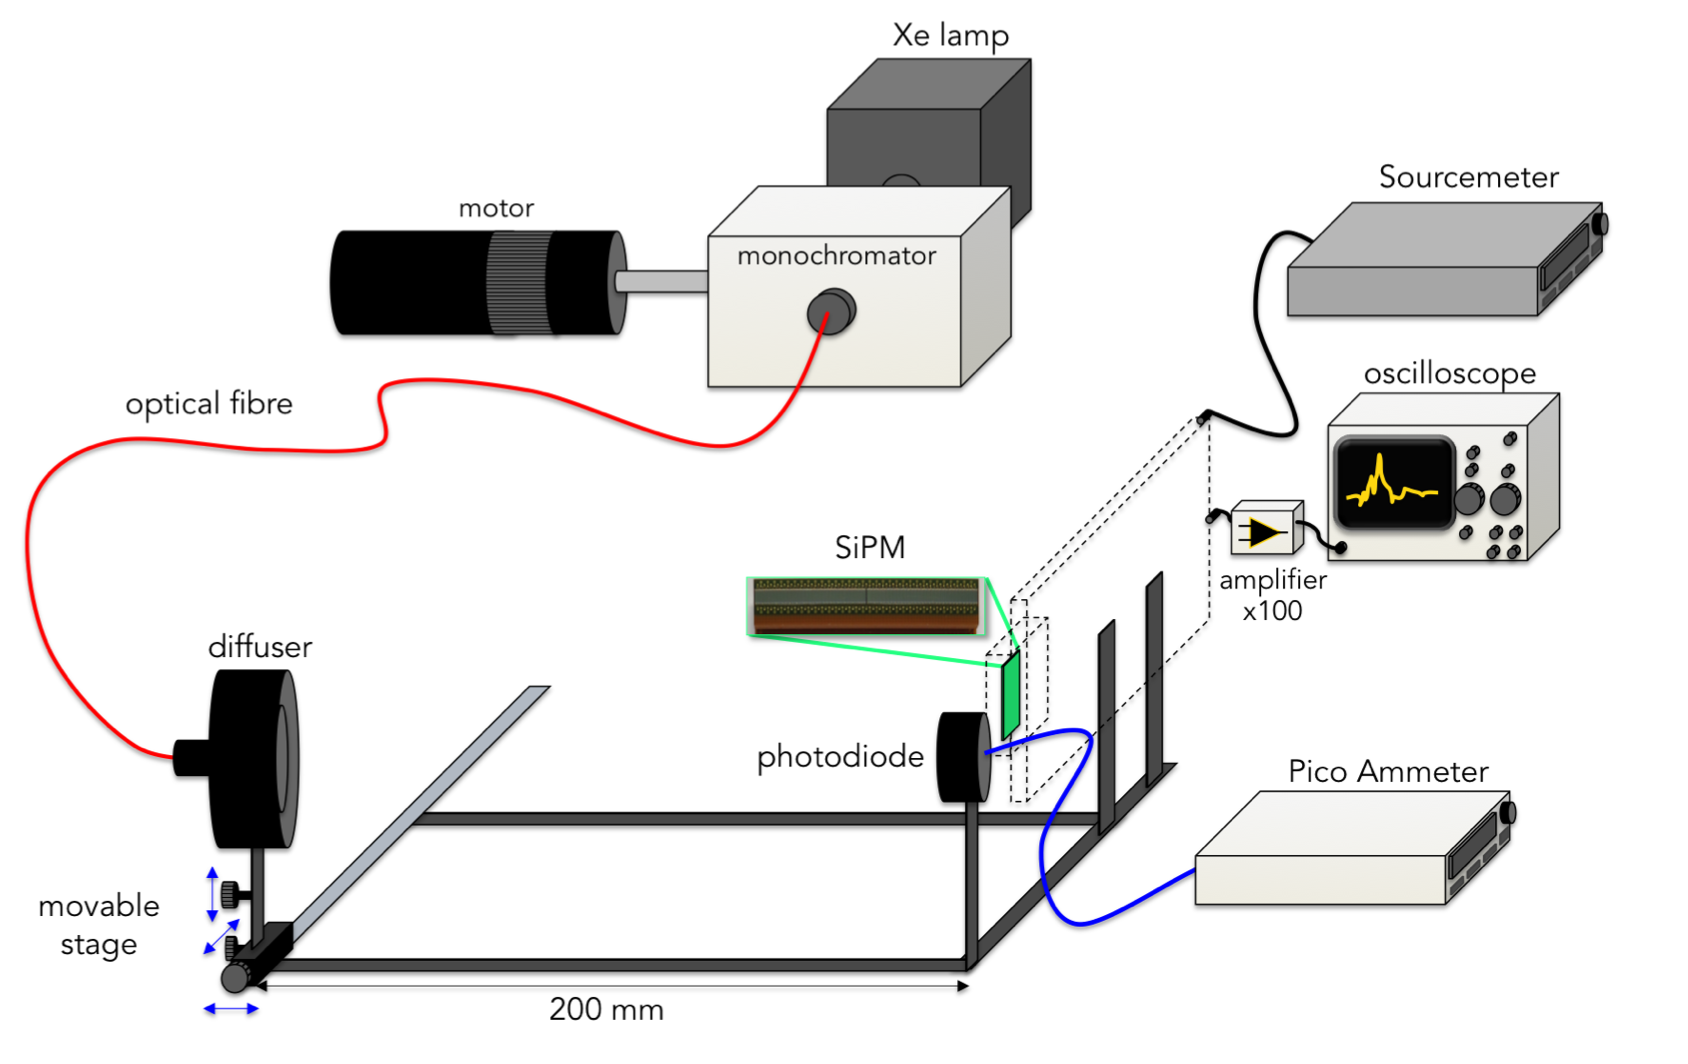
\includegraphics[width=\textwidth]{gfx/schemes/PDEsetupsketch.png}
    \caption{Scheme of the PDE setup \cite{Girard2018CharacterisationDistributions}.}
    \label{fig:PDE setup sketch}
\end{figure} 

A picture of the setup is shown in Fig. \ref{fig:PDE setup pic} and a scheme in Fig. \ref{fig:PDE setup sketch}. The light source is a Xe lamp that passes trough a monochromator\footnote{H10-UV Yvon Jobin} allowing to select a narrow wavelength interval ($\pm 1$nm). The monochromatic light now goes through a diffuser via an optical fibre. The diffused light is projected on the SiPM and a PIN diode of \SI{10.3}{mm} diameter is used for calibration\footnote{The diffuser has changed compared to \cite{Girard2018CharacterisationDistributions}.}. It is sensible from \SI{160}{\nano m} to \SI{900}{\nano m} and its photo-current is measured with a pico ammeter\footnote{KEITHLEY 6485 PICOAMMETER}. 


Three different measurements are taken to acquire the needed data for the gain and PDE. First, the diode calibration data consists in measuring the current produced by the PIN diode for each wavelength $\lambda$.  As Eq. \eqref{eq:Frequency PDE} and Eq. \eqref{eq:Current PDE} show, calibration data from the PIN Diode is crucial (dependency of $I_{PD}(\lambda)$), because this calibration allows to know how many photons are projected on the SiPM surface $A_{SiPM}$. The calibration data should be taken regularly, with a constant temperature during the measurement, fixed at $T_{meas} = 25.0 ^{\circ}$C.
\\
After the calibration comes the acquisition of the dark count rate and dark current of the studied detector. As in \ref{ch:Experimental methods:Noise identification}, a black cloth is wrapped around the detector so that only noise is present. The oscilloscope counts the number of peaks higher than $0.6$PE for a time window of \SI{100}{\micro s} for every $\Delta V$. In the mean time, the current produced by the SiPM is recorded for every $\Delta V$ too.
\\
The third and last measurement is the "light" data. The SiPM is placed in front of the diffuser and the measurement are the same as in the dark but now for all $\lambda$ in addition to every $\Delta V$.
\\
As mentioned before, the PIN Diode and the SiPM are mounted on motorized rails. The light beam should be perfectly aligned with the measured device. One can plot the current of the SiPM and PIN Diode as a function of the horizontal position, shown in Fig. \ref{fig:light alignment positions}
\begin{figure}[http]
    \centering    
    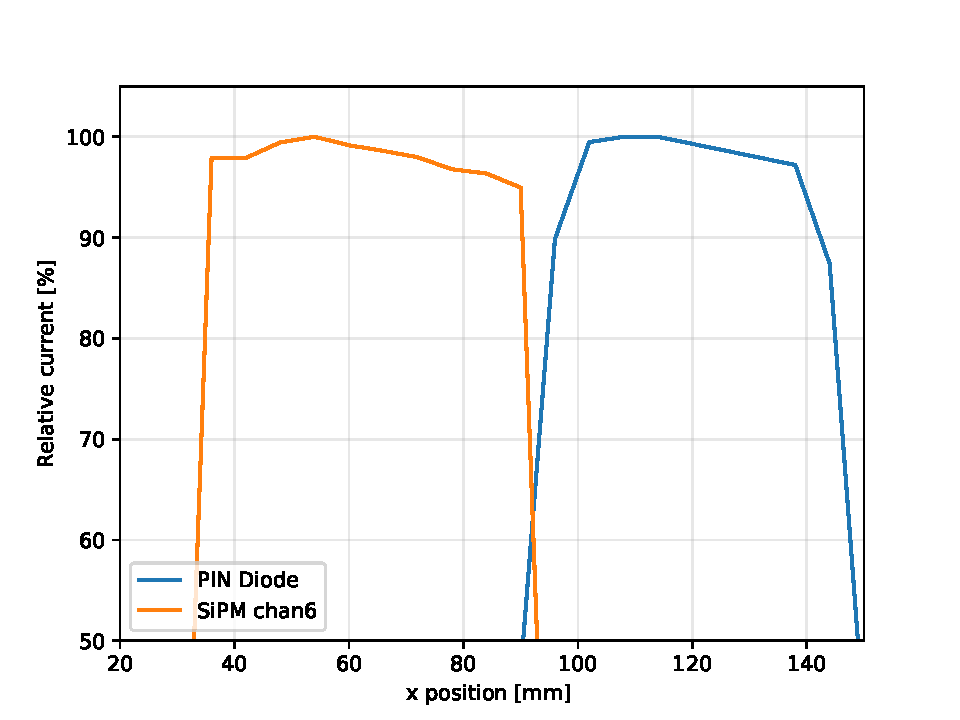
\includegraphics[width=0.8\textwidth]{gfx/plots/positions.pdf}
    \caption{Measured relative photo-current of the PIN diode and the SiPM as a function of the horizontal position. }
    \label{fig:light alignment positions}
\end{figure}
Hence, from this plot the position for the perfect alignment can be found for the channel $6$  which is $60 $ mm and the PIN Diode $120 $ mm. The same can be obtained for any channel as Eq. \eqref{eq:light alignement} shows (position in mm):

\begin{equation}
    x(channel) = 60 - channel\cdot250\cdot 10^{-3}
    \label{eq:light alignement}
\end{equation}

%\textbf{Better homogeneity plot}
%\textbf{Add a H. plot for the H2017}


\subsection{Gain}
\label{ch:experiement methods:Gain & PDE:gain}
The gain is measured with the light data and computed as in Eq. \eqref{eq: gain computation}. For each $\Delta V$ and $\lambda$, the photo-current $I_{light}(\Delta V, \lambda)$ is measured and corrected with the proportion of DiXT. $P_{DiXT}(\Delta V)$ is the probability of direct cross talk measured in the waveform analysis (see \ref{section:waveform analysis}). This corrected value is divided by $F_{light}$ which is the rate of peaks over the time interval selected by the oscilloscope (\SI{100}{\micro s}). The ratio: $$\frac{I_{light}(\Delta V, \lambda)\cdot(1-P_{DiXT}(\Delta V))}{F_{light}}$$ is then the total charge generated. To finally get the gain, we divide the total charge by the elementary charge $e$. No significant variations are observed with $\lambda$ so we take the average over $\lambda$: 
\begin{equation}
    G_{light}(\Delta V) = \frac{I_{light}(\Delta V)\cdot(1-P_{DiXT}(\Delta V))}{ F_{light}(\Delta V)\cdot e}
    \label{eq:gaincomputation}
\end{equation}

\paragraph{uncertainties.} The statistical uncertainties are again negligible since the they represents $0.1\%$. By measuring the several times the gain, the systematics uncertainties are estimated at $2\%$. Results are presented in \ref{ch:Results:Gain}.


\subsection{Photo-Detection Efficiency} 
\label{ch:experiement methods:Gain & PDE:PDE}

There are two ways of measuring the PDE:

\paragraph{Current method:} The current method uses the current recorded from the light and dark data explained in \ref{ch:Experimental methods:Gain and PDE:setup}. 
It exploits the measurement on the gain value $G_{light}(\Delta V)$, measured as described in section \ref{ch:experiement methods:Gain & PDE:gain}. 
Where $I_{PD}(\lambda)$ is the current produced by the PIN diode in the calibration data. $A_{PD}$ and $A_{SiPM}$ are the areas of the PIN diode and the SiPM channel respectively. 
The correction on the current takes into account the primary and secondary noises. The measured current $I^*$ corresponds to Eq. \eqref{eq: correction measured current}
\begin{equation}
    I^{*}= I_{light}\cdot(1+ r_{current})
    \label{eq: correction measured current}
\end{equation}
\begin{equation*}
    r_{current } =P_{DeXT} + P_{DiXT}+ w_{AP}\cdot P_{AP} + w_{ho}\cdot P_{ho}
    \label{eq: correction r current}  
\end{equation*}
Where $ w_{AP}$ \& $w_{ho}$ are the mean amplitude of the after-pulse and higher order peaks respectively.
At first approximation (since $r_{current} \ll 1$), taking into account the measured dark current $I_{DCR}$, the current is then corrected as Eq.\eqref{eq:correction I}:
\begin{equation}
    I_{light} = (I^{*}-I_{DCR})\cdot(1-r_{current})
    \label{eq:correction I}
\end{equation}
These values of amplitude and probabilities are measured in \ref{ch:Experimental methods:Noise identification}.

The final equation for the current PDE is then Eq. \eqref{eq:Current PDE}:
\begin{equation}
    \texttt{PDE}_{curr}(\Delta V, \lambda) = \frac{\left(I^{*}(\Delta V, \lambda)-I_{DCR}(\Delta V)\right)\cdot(1-r_{current}(\Delta V))}{I_{PD}(\lambda)\cdot G_{light, mean}(\Delta V)}\cdot \frac{A_{PD}}{A_{SiPM}} 
    \label{eq:Current PDE}
\end{equation}


\paragraph{Rate method:} For each wavelength $\lambda$, and each over voltage $\Delta V$, the number of peaks are counted by the oscilloscope on a given time window of $\Delta t =$ \SI{100}{\micro s}. This allows to not correct for DiXT since only peaks above a $0.6$PE thresholds are counted and not their amplitude. The rate is obtained by counting the peak on a given time window. The rate in the dark is called $F_{DCR}$ while the rate in the SiPM illuminated is called $F_{light}$. 
As for the current method, the measured rate $F^*$ do not correspond to the rate produced $F_{light}$ only by light detection. It needs to be corrected as in Eq. \eqref{eq:rate correction}:
\begin{equation}
    F^{*} = F_{light}\cdot(1+ r_{rate})
    \label{eq:rate correction}
\end{equation}
\begin{equation*}
    r_{rate} = P_{DeXT} + P_{AP}^{0.6} +P_{ho}^{rate}
    \label{eq: correction r current}  
\end{equation*}
Therefore, the rate in the light corrected is given by Eq. \eqref{eq:rate light}:
\begin{equation}
    F_{light}= (F^* - F_{DCR})\cdot(1-r_{rate})
    \label{eq:rate light}
\end{equation}
The equation to calculate the PDE using this method is: Eq. \eqref{eq:Frequency PDE}. 
\begin{equation}
    \texttt{PDE}_{freq}(\Delta V, \lambda) = \frac{\left(F^{*}(\Delta V, \lambda)-F_{DCR}(\Delta V)\right)\cdot(1-r_{rate}(\Delta V))}{e \cdot I_{PD}(\lambda)}\cdot \frac{A_{PD}}{A_{SiPM}}
    \label{eq:Frequency PDE}
\end{equation}
The rate method does not require the gain and then the uncertainties are reduced. For noise measurements with a large amount higher order peaks, the PDE may over correct as overvoltage increases resulting in an underestimation of PDE. A fine tuning of the thresholds in the waveform analysis needs to be done to get accurate PDE results. 
Results are presented in \ref{ch:Results:PDE}.

\chapter{Results and Discussion}
\label{ch:Results}
This chapter is dedicated to the presentation of the results obtained from characterised detectors. The quenching resistor measurement is in section \ref{ch:Results:Rq}, the breakdown voltage in section \ref{ch:Results:breakdown voltage}, Noise Classification in section \ref{ch:Results:Noise Classification}, and the gain and PDE in sections \ref{ch:Results:Gain} \& \ref{ch:Results:PDE}.

\section{Quenching resistor}
\label{ch:Results:Rq}
 In this section, the quenching resistor measurements of the FBK and Hamamatsu SiPMs are presented. It has been measured with two different methods: from the IV curve in forward bias (see \ref{ch:experiement methods:IV:Rq IV}) and from the waveform analysis (see \ref{ch:experiement methods:WA:Rq WA}).  
 
\subsection{IV curve method} 
The results for the quenching resistors from the IV curve are shown in Fig. \ref{fig:IV curve linear fit and RQ}. The left plots are the IV curve in forward bias and the linear fits. The fitting range has been chosen from $0.5$ to $-2.3$ V for the FBK as discussed with S.Merzi \cite{StefanoMerzi2023PrivateCommunication}. For the Hamamatsu, the fitting range is the same as in \cite{Girard2018CharacterisationDistributions}.
% kind of IV talk 
The IV measurements shown in Fig. \ref{fig:IV curve linear fit and RQ} showed a very high dependency on the choice of the fitting range because the IV curve is not perfectly linear. 
% channels talk
The distinction between the channels [$0,63$] and [$64,127$] is clearly visible, marked by a certain discontinuity in the middle of the plots. This is due to the dead gap separating the two parts of $64$ channels. 
The \SI{31}{\micro m} has a lower $R_Q$ value in the channels  [$0,63$], which is a behavior opposite to the \SI{16}{\micro m} or \SI{42}{\micro m}, this could be due to a different initial position in the wafer. 
The spread over the mean value of $R_Q$ for each channel can be computed and shown in Table \ref{table:Rq + spread}.
\begin{table}[htbp]
\centering
\begin{tabular}{|c|c|c|c|c|}
\hline
Detector            & H2017         & $16 \mu$m     & $31 \mu$m     & $42 \mu$m     \\ \hline
$<R_Q>$ [k$\Omega$] & $550$         & $436 $        & $444 $       & $503 $ \\ \hline
Spread [\%]         & $7.39$        &  $4.6$        & $4.5$        & $3.3$          \\ \hline
\end{tabular}
\caption{Mean $R_Q$ over the measured channel, and the spread $\frac{max(R_Q)-min(R_Q)}{<R_Q>}$. }
\label{table:Rq + spread}
\end{table}
Nevertheless, the discrepancies in the $R_Q$ values are less than $5\%$ for the FBK, which is acceptable. 
% odd and even talk H2017 IV
The hamamatsu H2017 measurement shows a clear difference of $R_Q$ between the odd and even channels, causing a higher spread. Differences in design between FBK and Hamamatsu are responsible for this distinction between odd and even channel that are present in Hamamatsu but not in FBK.


\newgeometry{left=2.2cm,right=2.2cm,top=2cm,bottom=2cm}
\begin{figure}[htbp]
  \centering
  \begin{subfigure}{0.48\textwidth}
    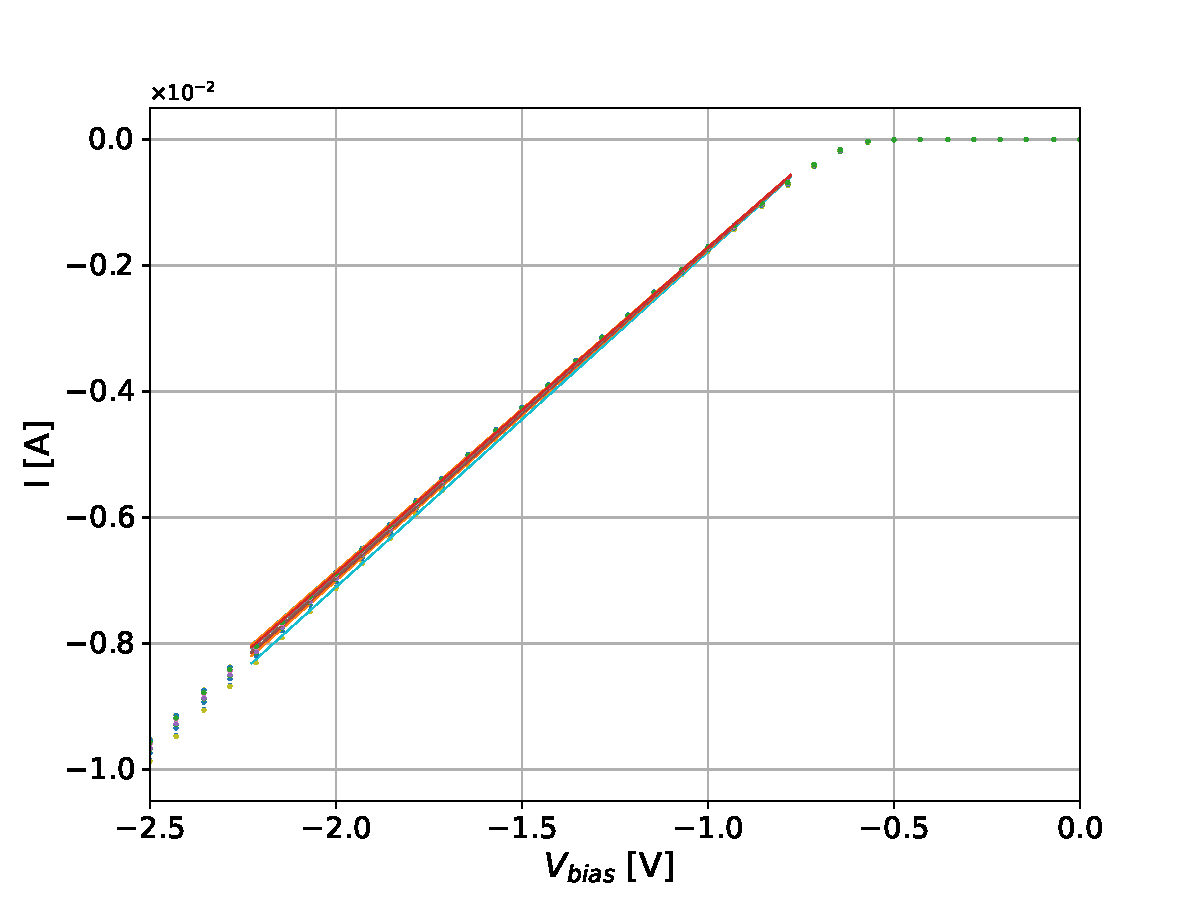
\includegraphics[width=\textwidth]{gfx/plots/Rq/16/FBK_16um_IV.pdf}
    \caption{IV curve linear fit \SI{16}{\micro m}.}
    \label{fig:}
  \end{subfigure}
  \hfill
  \begin{subfigure}{0.48\textwidth}
    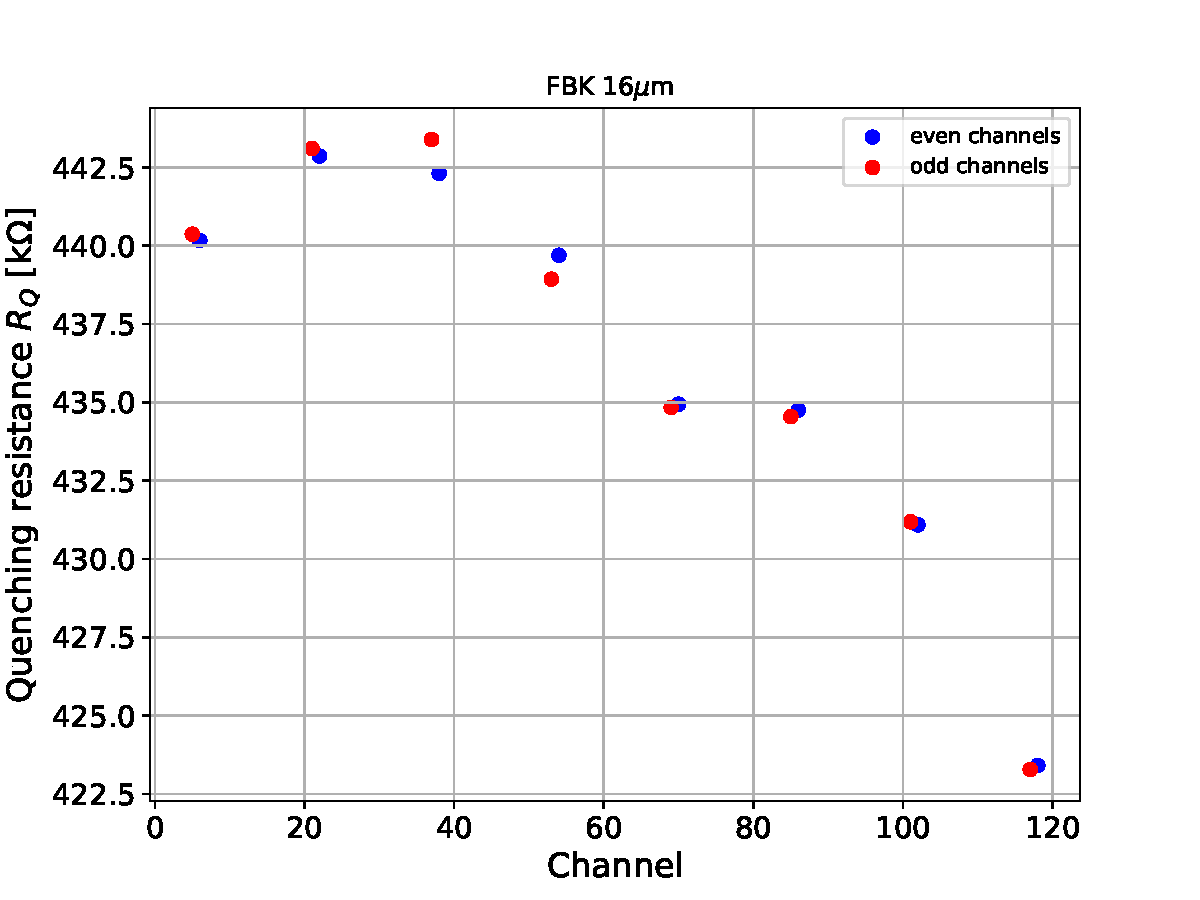
\includegraphics[width=\textwidth]{gfx/plots/Rq/16/FBK_16um_RQs.pdf}
    \caption{$R_Q$ results for \SI{16}{\micro m}.}
    \label{fig:}
  \end{subfigure}
  \begin{subfigure}{0.48\textwidth}
    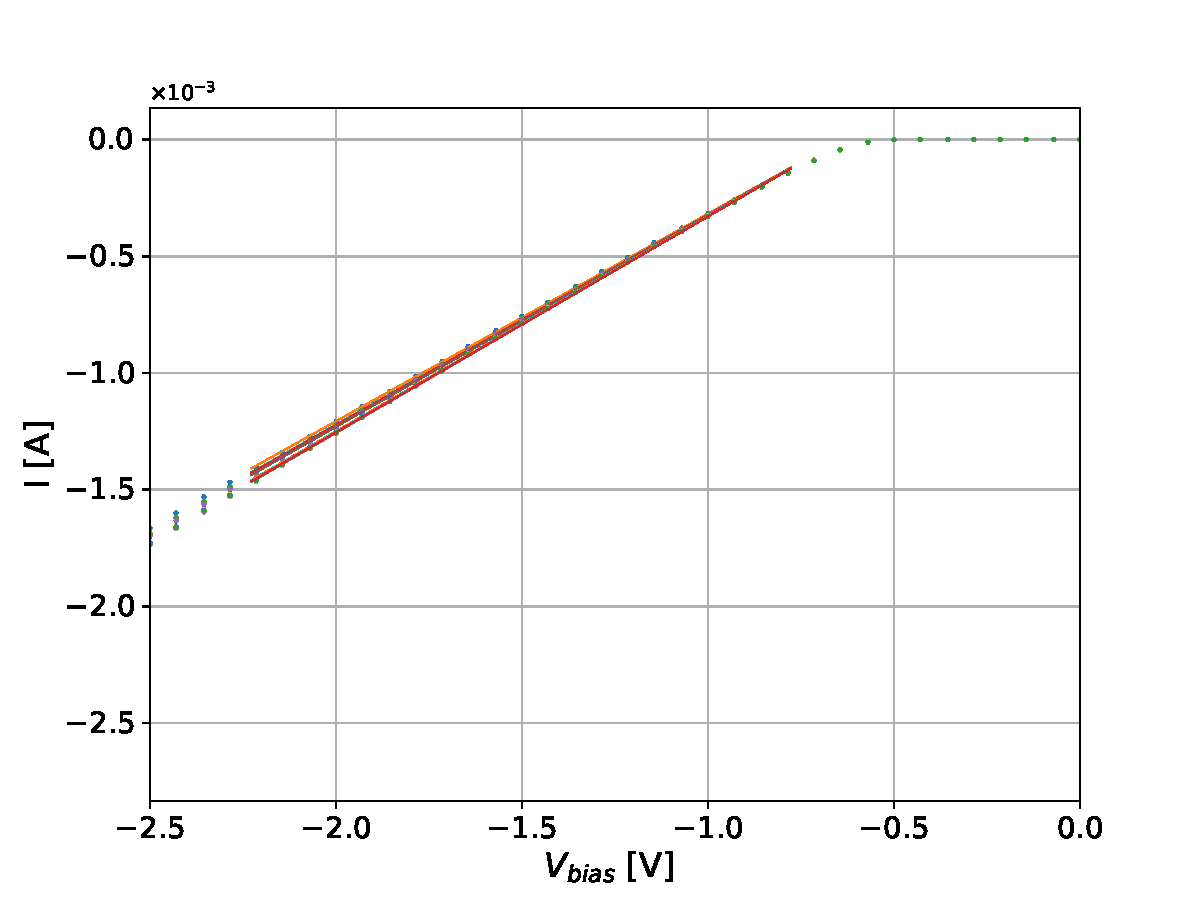
\includegraphics[width=\textwidth]{gfx/plots/Rq/31/FBK_31um_IV.pdf}
    \caption{IV curve linear fit \SI{31}{\micro m}.}
    \label{fig:}
  \end{subfigure}
  \hfill
  \begin{subfigure}{0.48\textwidth}
    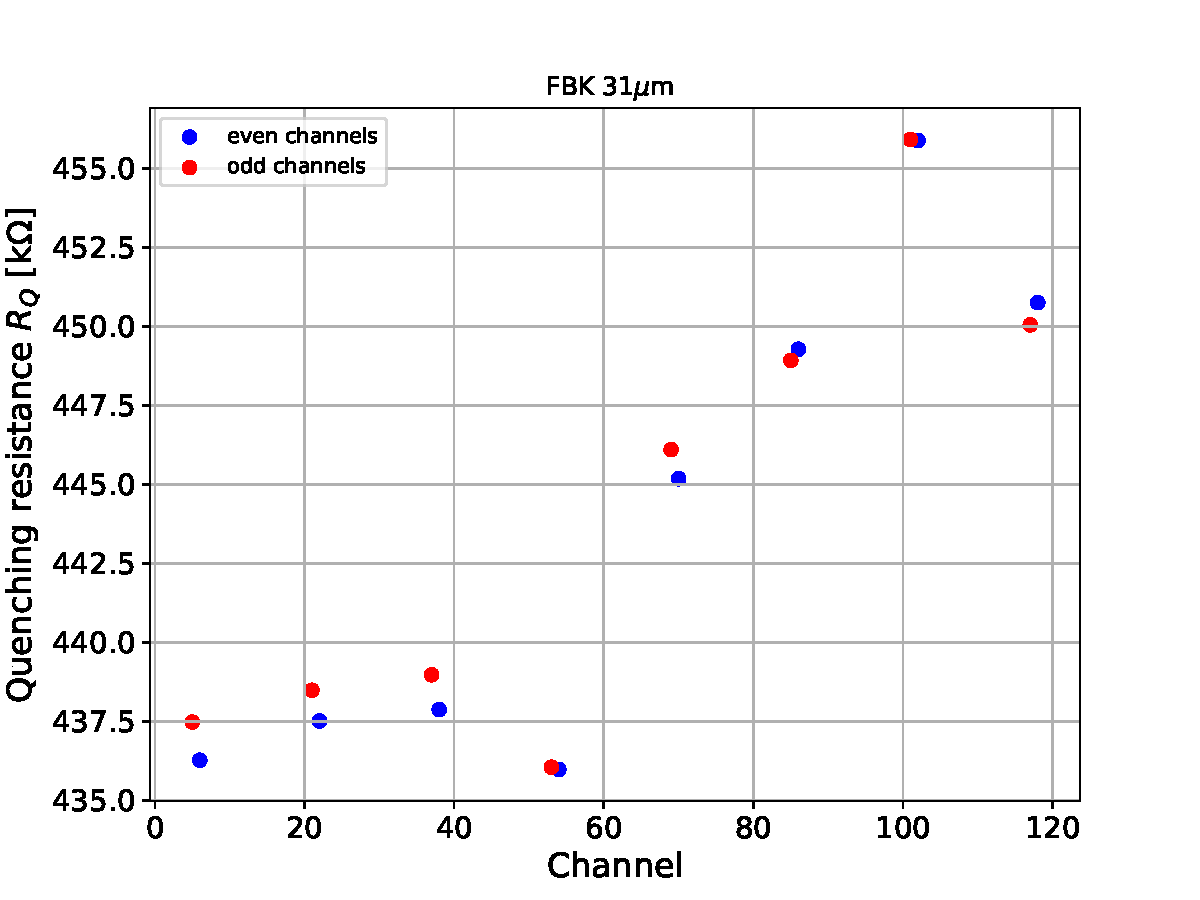
\includegraphics[width=\textwidth]{gfx/plots/Rq/31/FBK_31um_RQs.pdf}
    \caption{$R_Q$ results for \SI{31}{\micro m}.}
    \label{fig:}
  \end{subfigure}
  \begin{subfigure}{0.48\textwidth}
    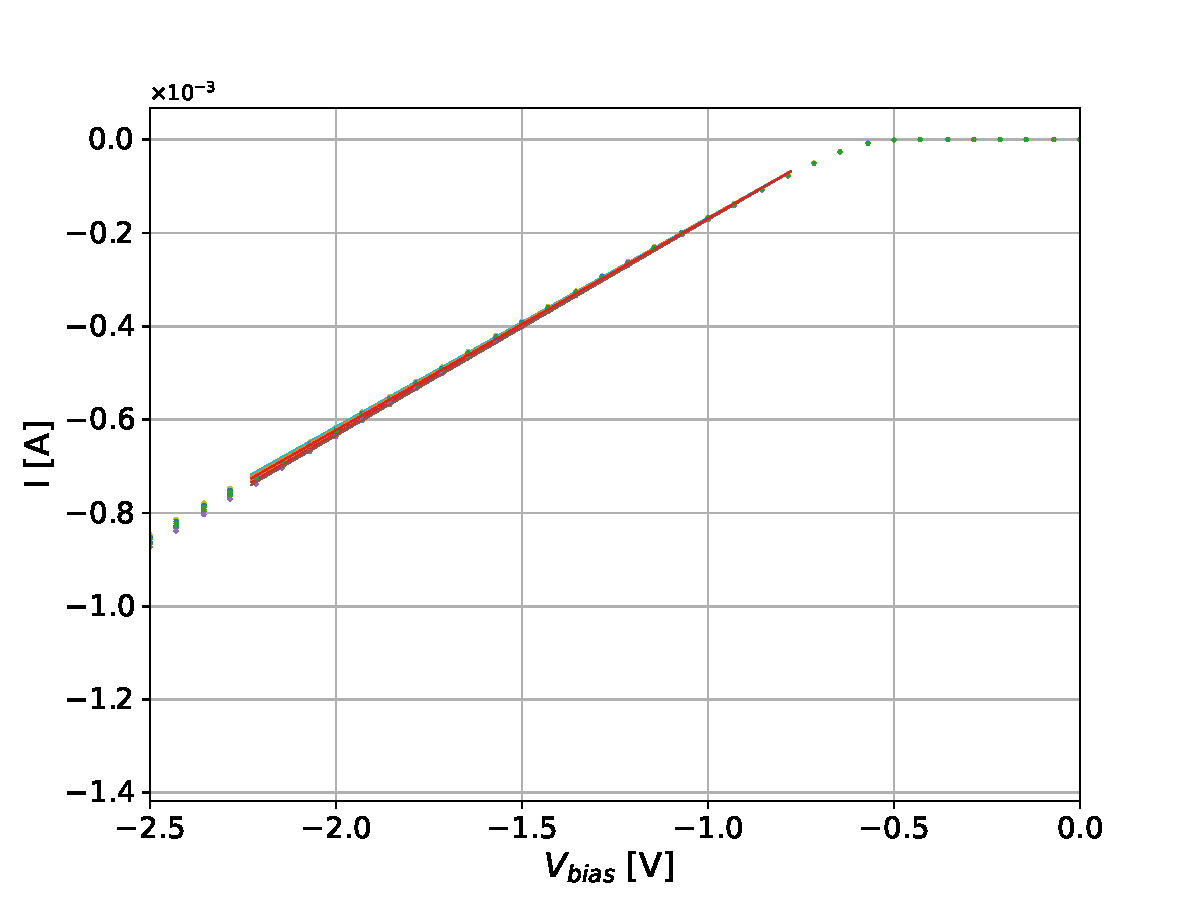
\includegraphics[width=\textwidth]{gfx/plots/Rq/42/FBK_42um_IV.pdf}
    \caption{IV curve linear fit \SI{42}{\micro m}.}
    \label{fig:}
  \end{subfigure}
  \hfill
  \begin{subfigure}{0.48\textwidth}
    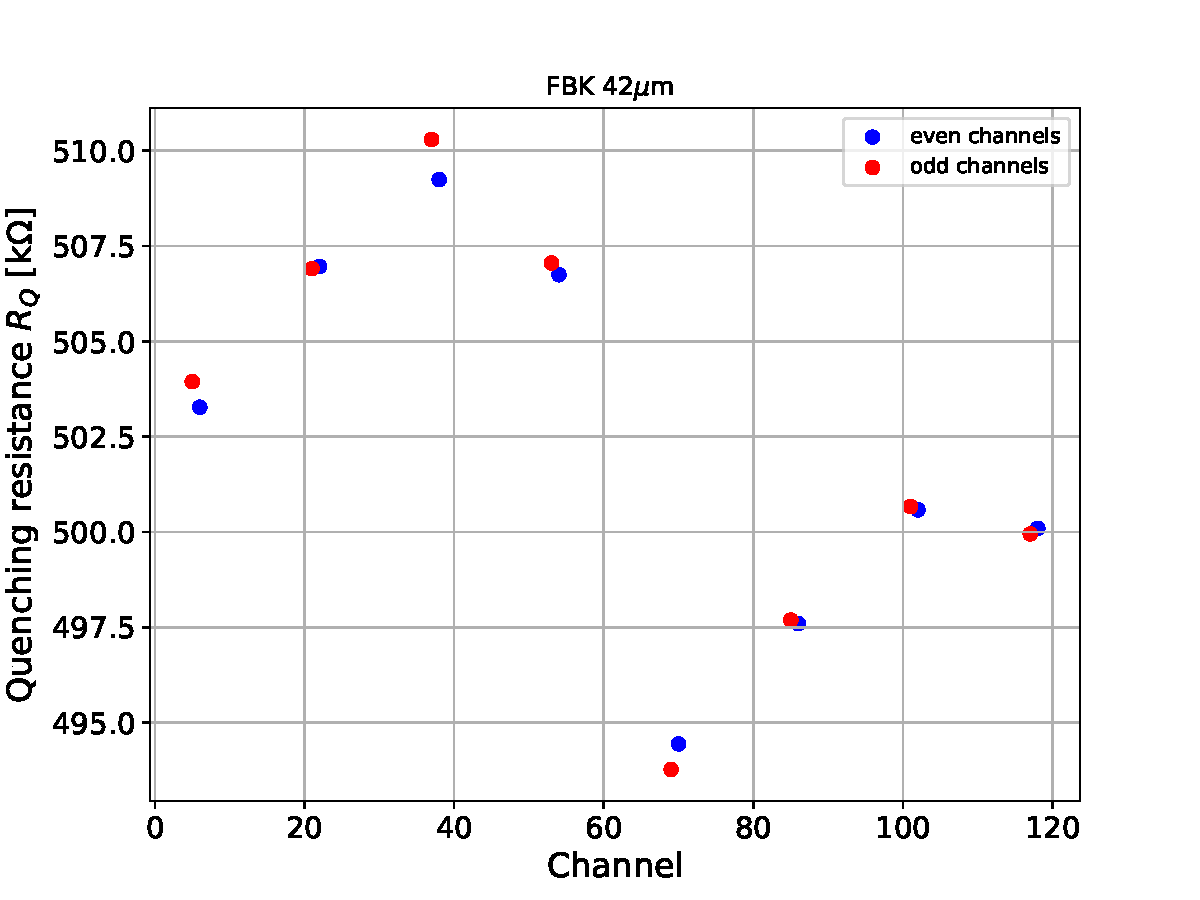
\includegraphics[width=\textwidth]{gfx/plots/Rq/42/FBK_42um_RQs.pdf}
    \caption{$R_Q$ results for \SI{42}{\micro m}.}
    \label{fig:}
  \end{subfigure}
  \begin{subfigure}{0.48\textwidth}
    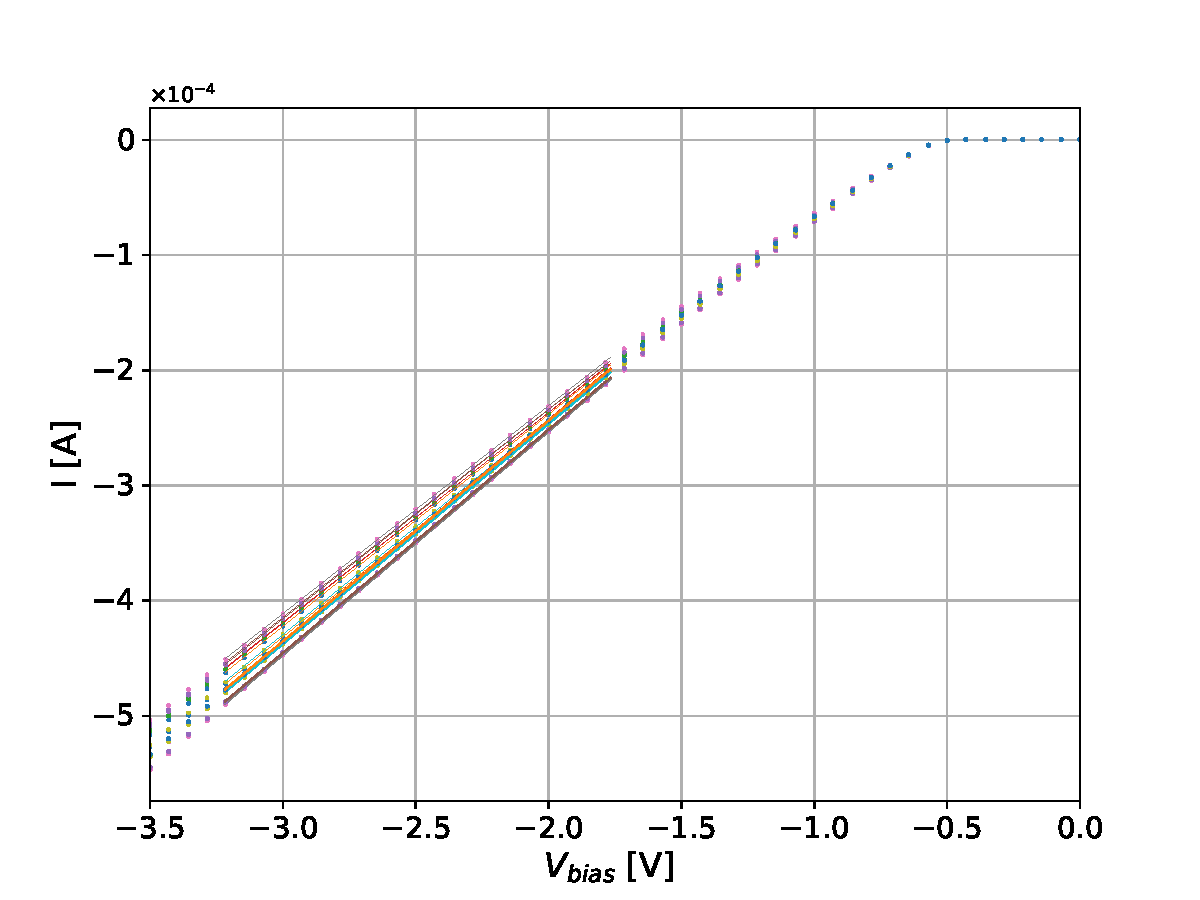
\includegraphics[width=\textwidth]{gfx/plots/Rq/H2017/FBK_2017um_IV.pdf}
    \caption{IV curve linear fit H2017.}
    \label{fig:}
  \end{subfigure}
  \hfill
  \begin{subfigure}{0.48\textwidth}
    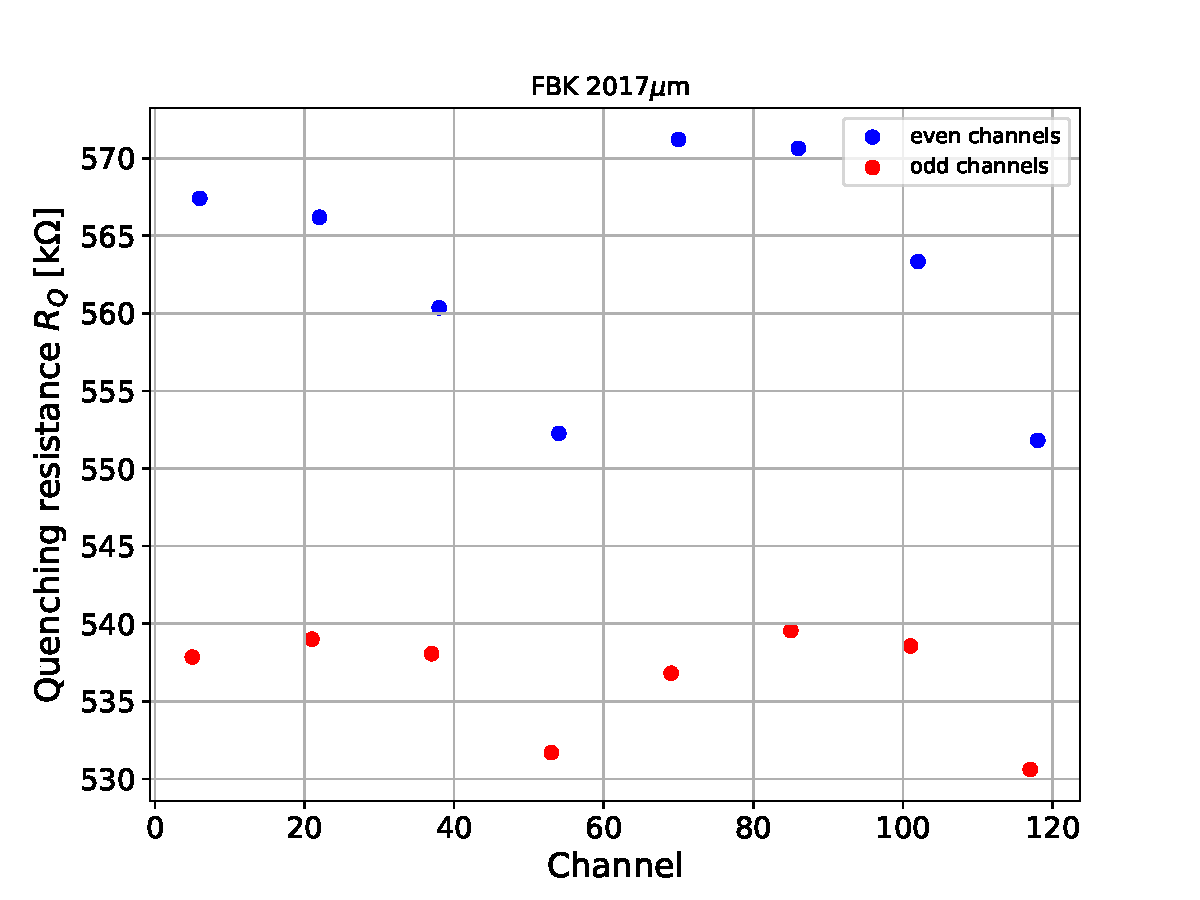
\includegraphics[width=\textwidth]{gfx/plots/Rq/H2017/FBK_2017um_RQs.pdf}
    \caption{$R_Q$ results for H2017.}
    \label{fig:}
  \end{subfigure}
  \caption{Plots of the IV curve fits (left) and the quenching resistor (right) for all detectors.}
  \label{fig:IV curve linear fit and RQ}
  
\end{figure}

\restoregeometry

\subsection{Time constant method}
 For the time constant methods, the results are shown in Table. \ref{table:taulongs table} and Fig. \ref{fig:tau longs}.
\begin{figure}[htbp]
    \centering
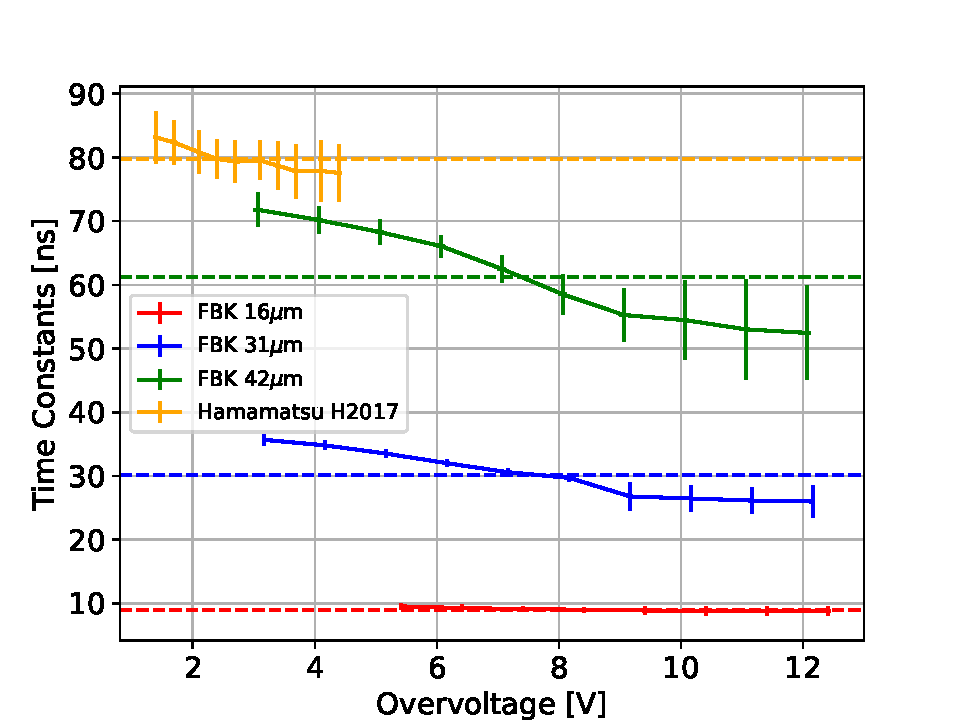
\includegraphics[width=\textwidth]{gfx/plots/WA/taulongs.pdf}
    \caption{$\tau_{long}$ as a function of $\Delta V$ for every detectors.}
    \label{fig:tau longs}
\end{figure}
\begin{table}[htbp]
\begin{tabular}{|c|c|c|c|c|}
\hline
\textbf{}                         & \textbf{FBK \SI{16}{\micro m}} & \textbf{FBK \SI{31}{\micro m} }        & \textbf{FBK \SI{42}{\micro m}} & \textbf{Hamamatsu H2017} \\ \hline
\textbf{$<\tau_{long}>$ {[}ns{]}} & $9 \pm 1.8$         & $30\pm 6$       & $61 \pm 12$        & $79.7 \pm 4$         \\ \hline
%\textbf{$C_d$}                    & $0.227\cdot 10^{-13}$  & $0.708\cdot 10^{-13}$ & $1.128\cdot 10^{-13}$  & $1.637\cdot 10^{-13}$    \\ \hline
\textbf{$R_Q$ {[}k$\Omega${]}}    & $396 \pm 87 $          & $422 \pm 93 $          & $497 \pm 109$           & $487\pm 19$             \\ \hline
\end{tabular}
\caption{$R_Q$ values for each detectors. With $20\%$ errors on $\tau_{long}$ (FBK) \& $2\%$ (for H2017) and $2\%$ errors on gain.}
\label{table:taulongs table}
\end{table}
% 1st results 
% tau long talk 
They were computed by measuring first the $\tau_{long}$ time constant with the waveform analysis. On Fig. \ref{fig:tau longs}, the different values as a function of overvoltage is shown for each detectors. A decrease of $\tau_{long}$ as $\Delta V$ increases is observable for all detectors.
In theory, $\tau_{long}$ should be constant, this results in large systematics errors of $20\%$ leading to measurement neither accurate nor satisfying.
%and should be further developed in a future work. 

% 4th comparison with manufacturer and guido. 
% fbk 
The manufacturer (FBK) \cite{StefanoMerzi2023PrivateCommunication} and Hamamatsu states a value of $R_Q = $ \SI{500}{\kilo \ohm}. 
% comparison with lois and guido 
The values for $R_Q$ are not perfectly \SI{500}{\kilo \ohm} due variations in the manufacture. For the FBK and Hamamatsu detectors, the IV measurements matches with the declared values with a spread below $5\%$ for the FBK. 
The measurements done by Loïs Niggli for the FBK detectors %\textbf{18\% span } 
\cite{NiggliLoisSECTIONIrradiation} are also compatible with what has been measured here. Also, the measurement in \cite{Girard2018CharacterisationDistributions} matches with the Hamamatsu too, with differences that can be due to the fact that the samples studied were different. 

% out look 
The measurement were not taken for all the possible channels, but this shows that the two methods presents similar results. The choice of one method to another depends on the aim of the measurement. Measuring with the IV curve allow to get the $\tau_{rec}$ which is equal to $\tau_{long}$. In the other way around, measuring first the $\tau_{long}$ with the waveform analysis leads to $R_Q$. Note that the IV measurement is way more easier to reproduce if the goal is to characterise more channels and having less systematic errors. The time constant method includes large errors from the gain but especially from the measured $\tau_{long}$. One could use the $R_Q$ values from the IV method to estimate the $\tau_{long}$ and compare it to the measured $\tau_{long}$ from the waveform analysis. 


\section{Breakdown Voltage}
\label{ch:Results:breakdown voltage}
This section presents the breakdown voltage measurements. Results are adjusted for a temperature of \SI{25.0}{\celsius}. In the Table. \ref{table:Vbds temp adjusted}, the measurement from the mean pulse amplitude described in \ref{ch:Experimental methods:breakdown voltage} are shown in the column "\textbf{WA}" and the fits are displayed in \ref{appendix:fig:Vbd fits}. One example is presented in Fig. \ref{fig:Vbd 31um chan6}. As comparison, the values from the $V_{bd}$ characterisation setup based on VATA64 taken by Guido Haefeli are shown in the column of the same name. 
\begin{figure}[htbp]
    \centering
    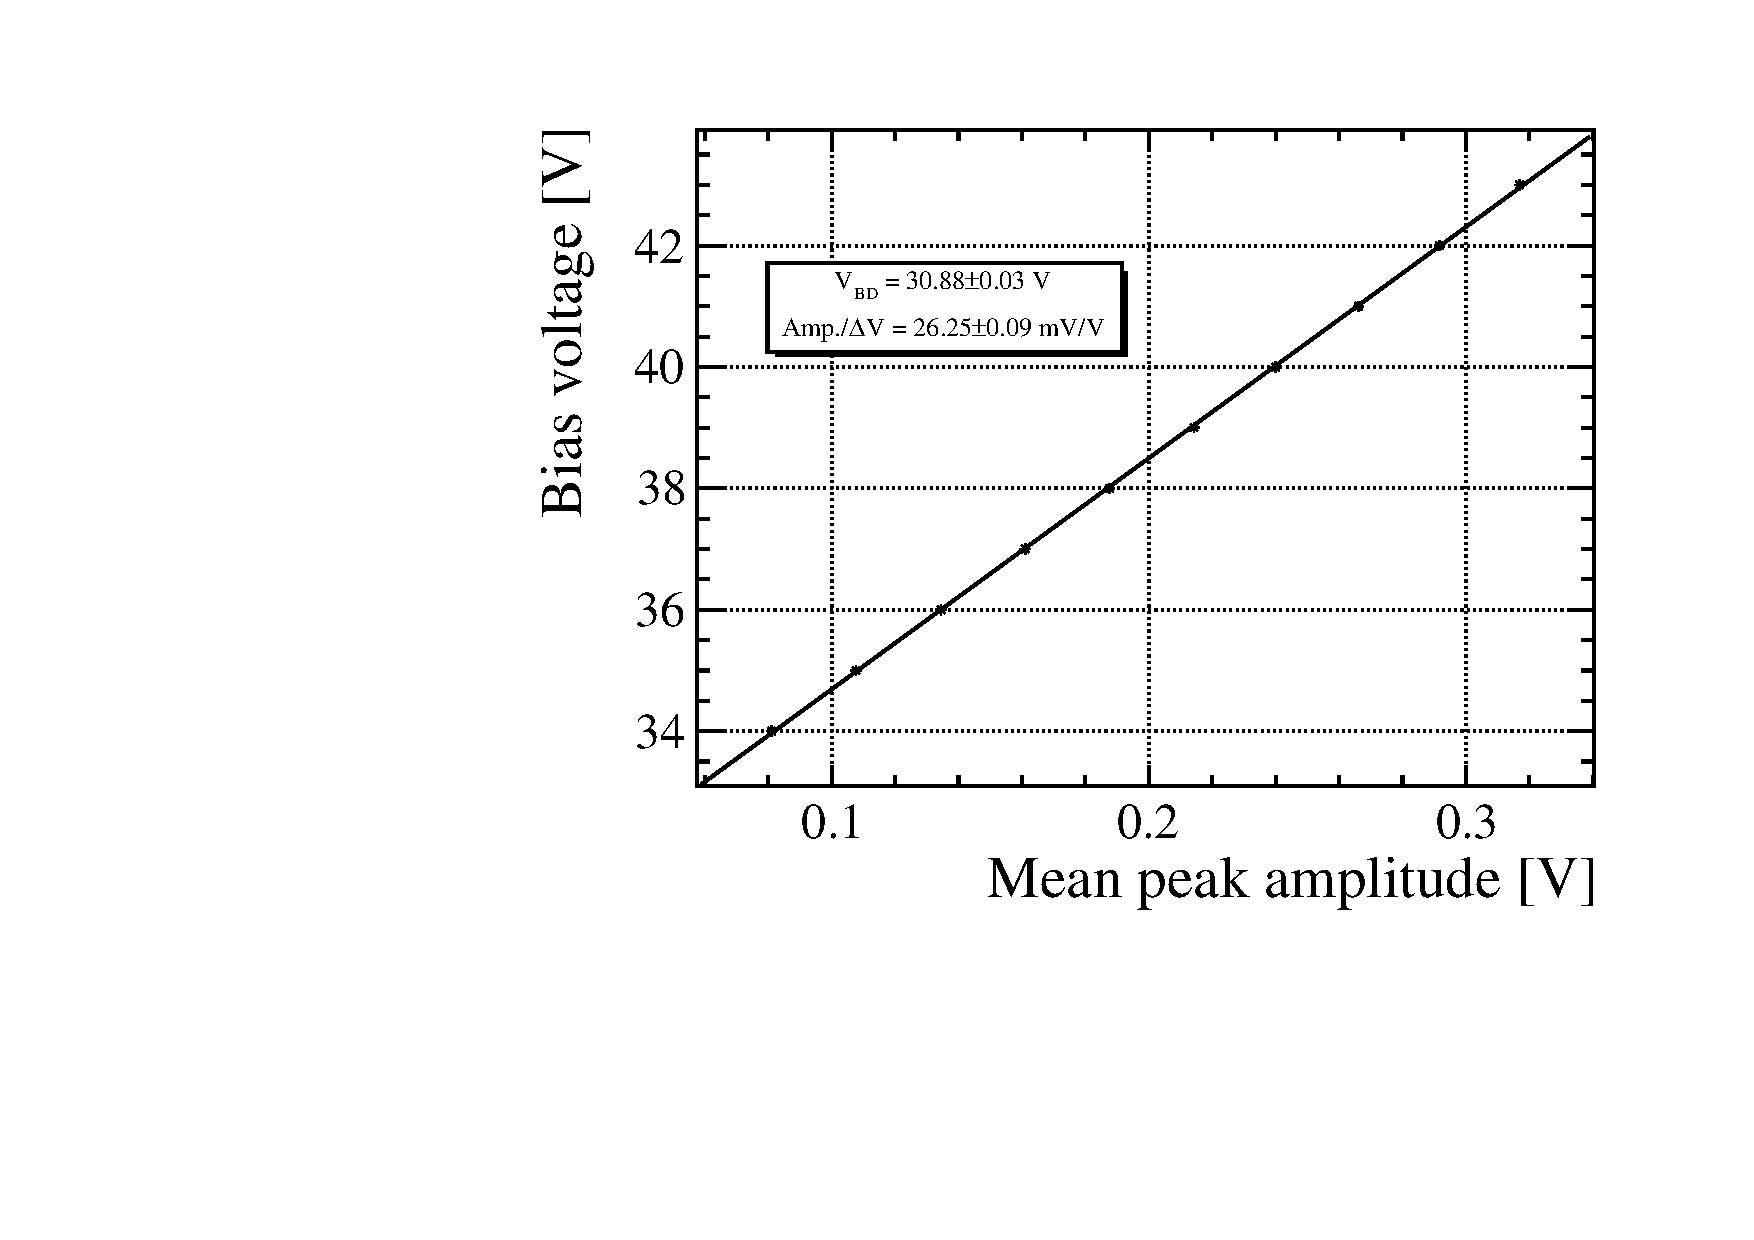
\includegraphics[width=0.7\textwidth]{gfx/plots/WA/31/Breakdown_voltage6.pdf}
    \caption{Breakdown voltage for the FBK \SI{31}{\micro m}, channel $6$.}
    \label{fig:Vbd 31um chan6}
\end{figure}

\begin{figure}[htbp]
  \centering
  \begin{subfigure}{0.48\textwidth}
    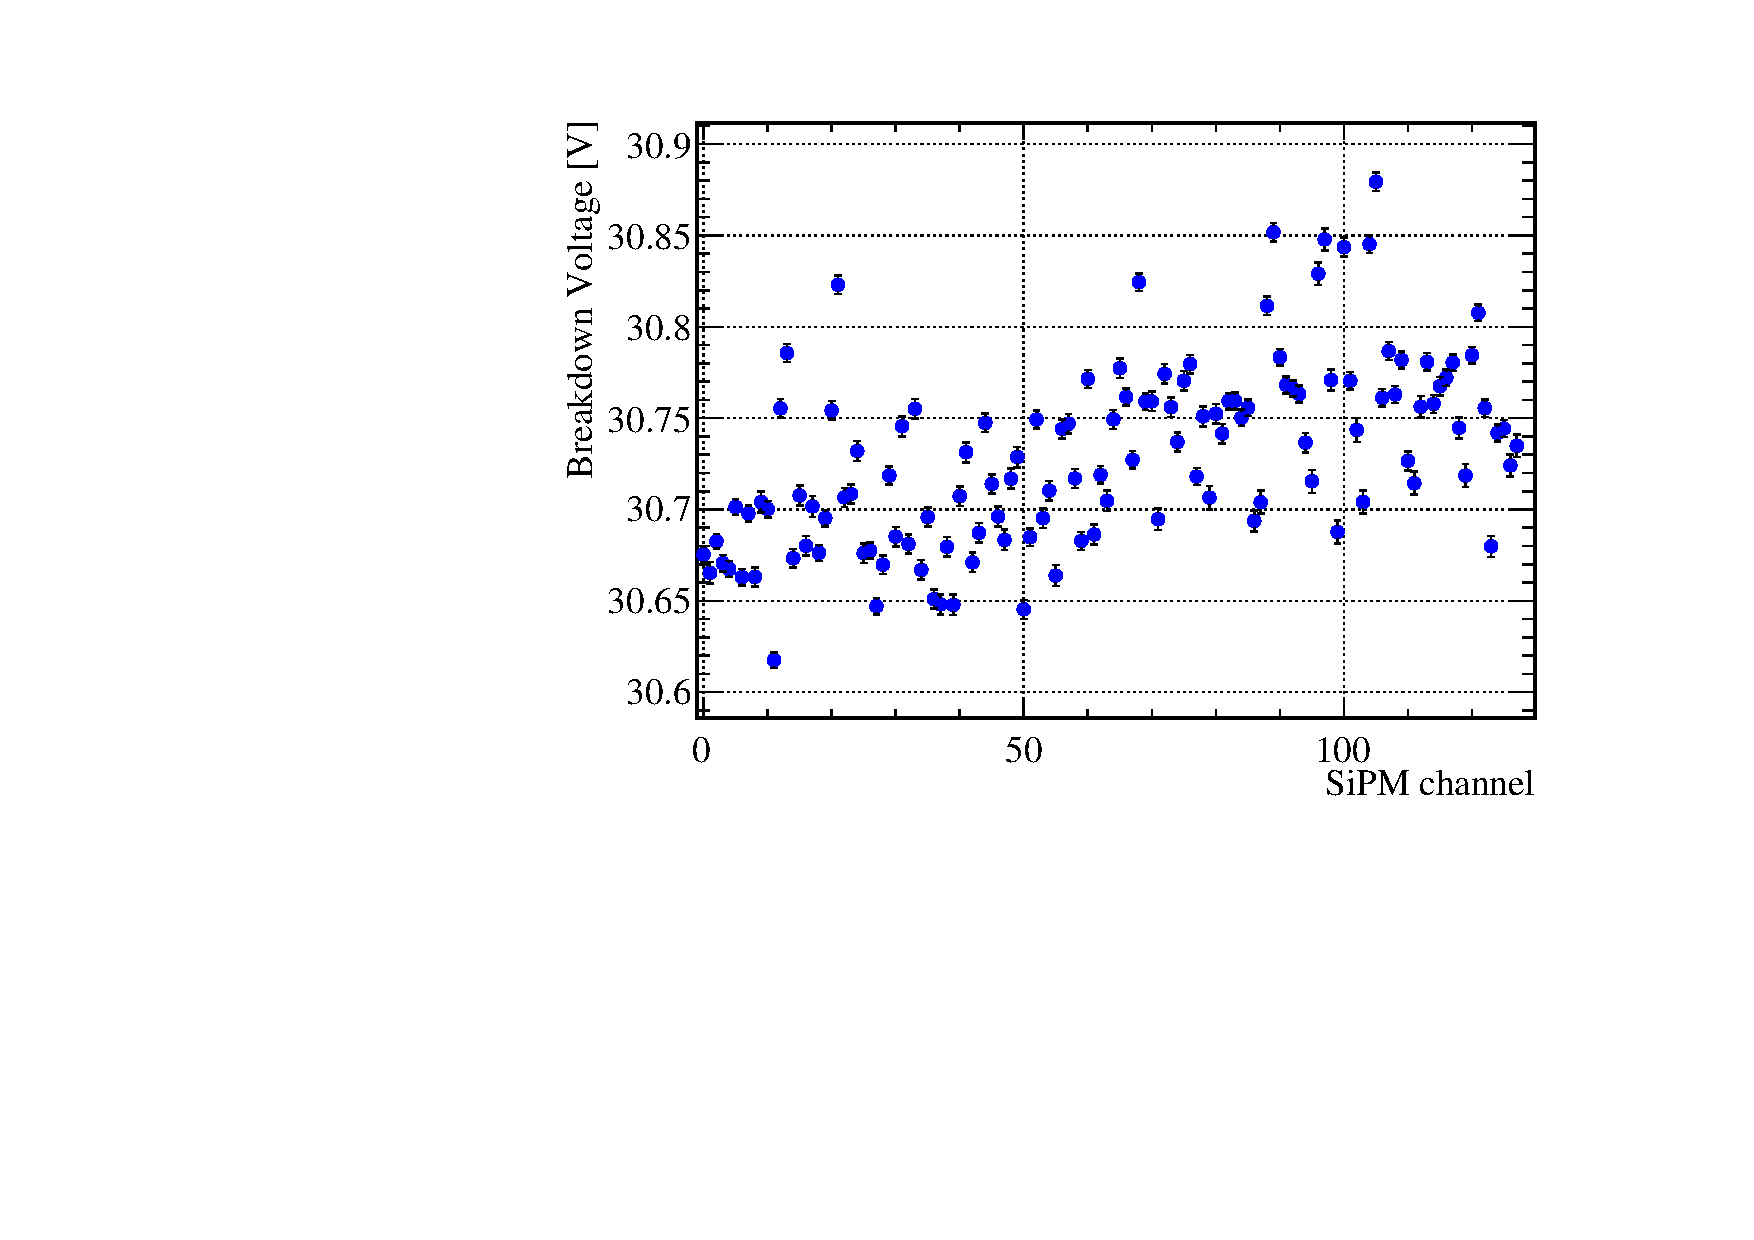
\includegraphics[width=\textwidth]{gfx/plots/WA/16/Vbd16.pdf}
    \caption{$V_{bd}$ \SI{16}{\micro m} sample $12$.}
    \label{fig:}
  \end{subfigure}
  \hfill
  \begin{subfigure}{0.48\textwidth}
    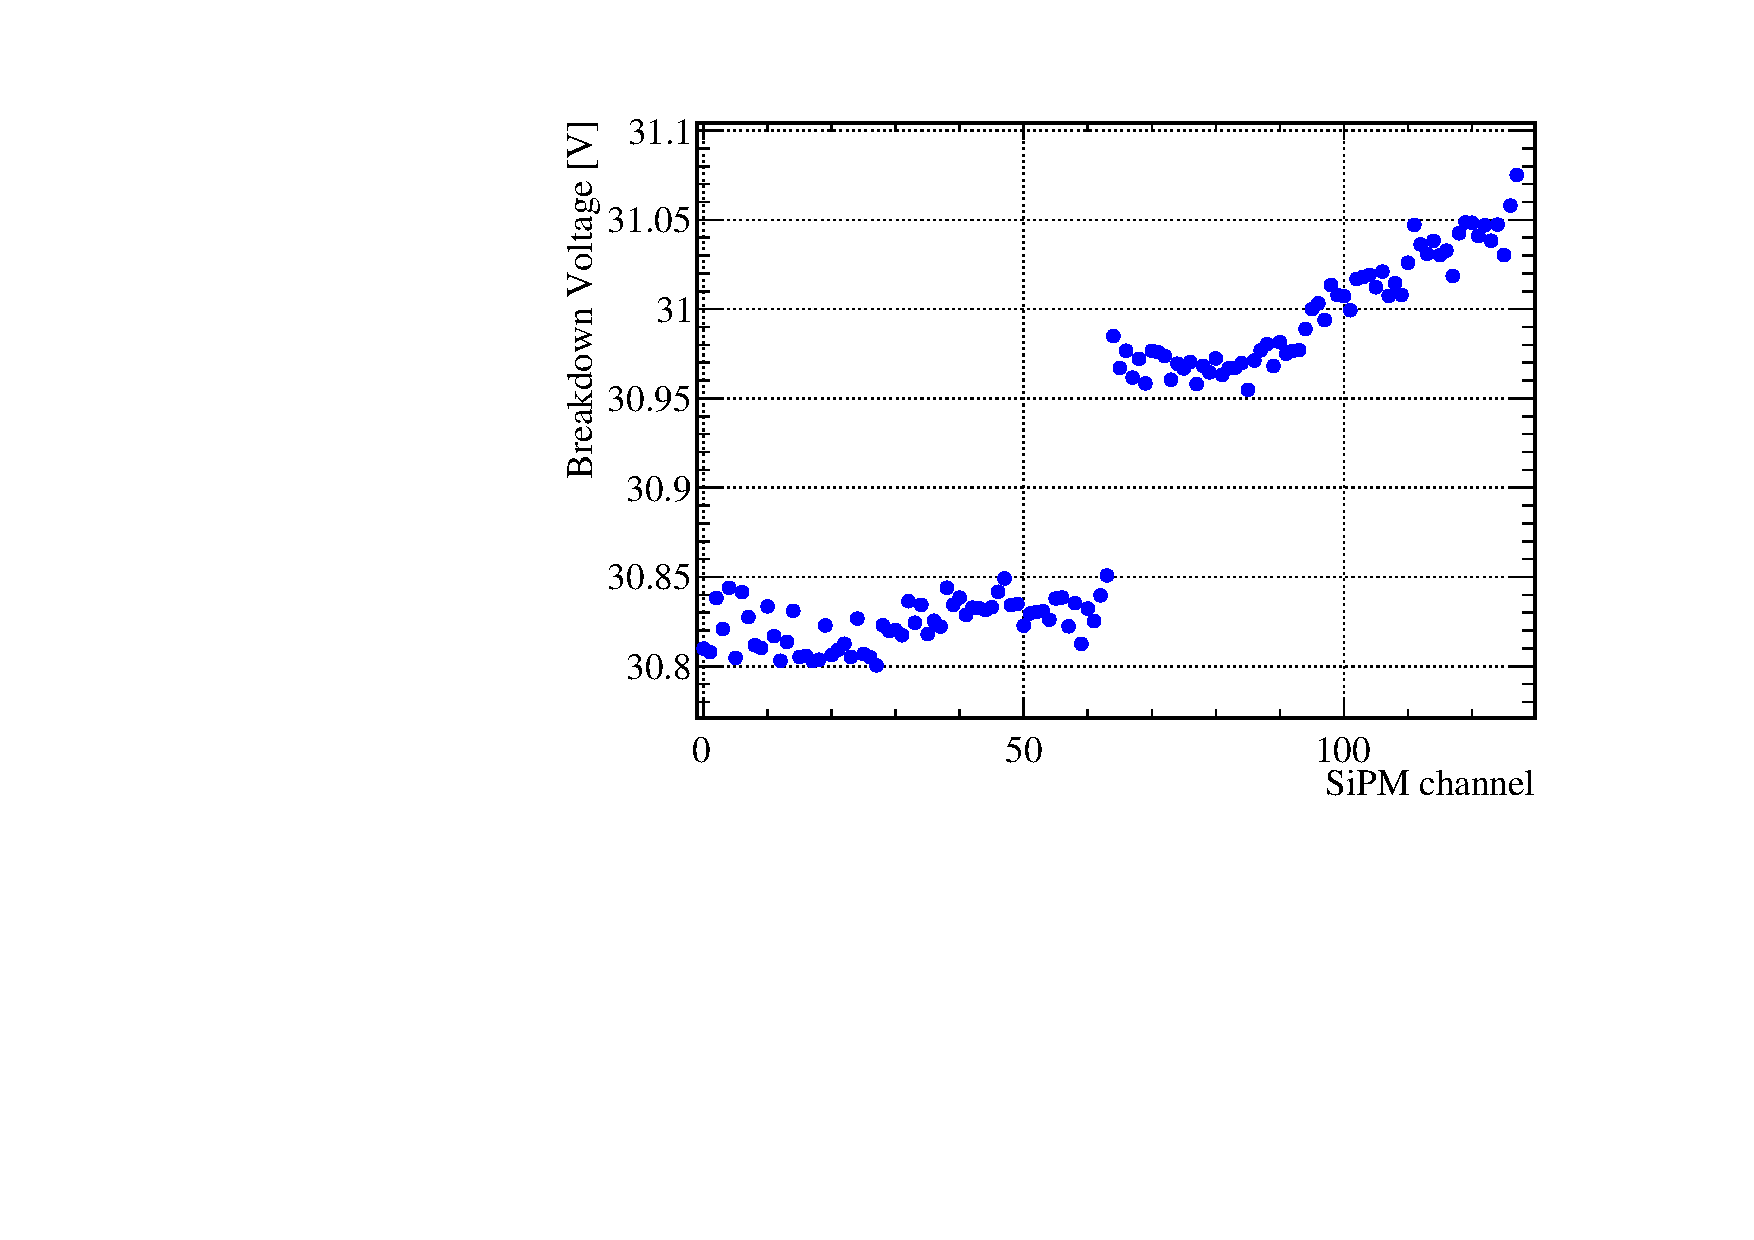
\includegraphics[width=\textwidth]{gfx/plots/WA/31/Vbd31.pdf}
    \caption{$V_{bd}$ \SI{31}{\micro m} sample $6$.}
    \label{fig:}
  \end{subfigure}
  \begin{subfigure}{0.48\textwidth}
    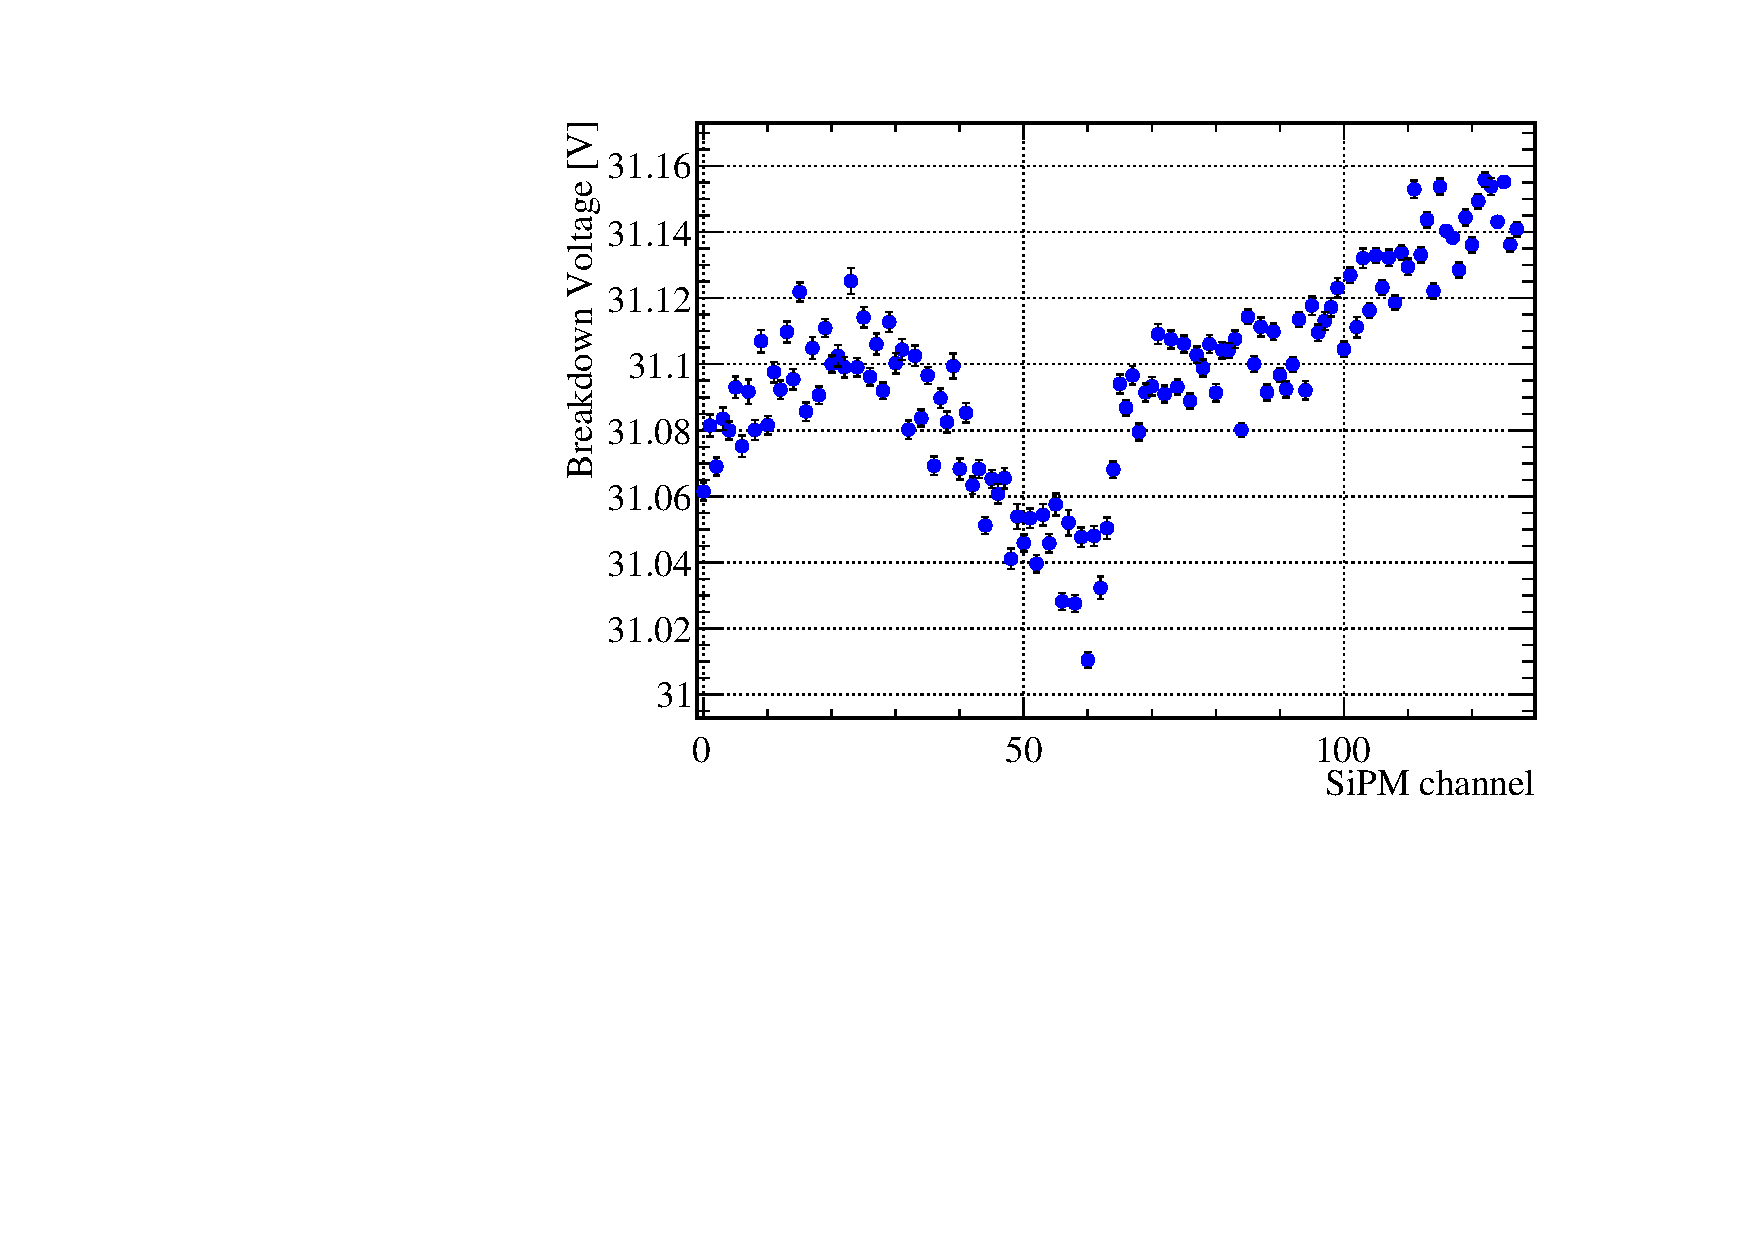
\includegraphics[width=\textwidth]{gfx/plots/WA/42/Vbd42.pdf}
    \caption{$V_{bd}$ \SI{42}{\micro m} sample $1$.}
    \label{fig:}
  \end{subfigure}
  \hfill
  \begin{subfigure}{0.48\textwidth}
    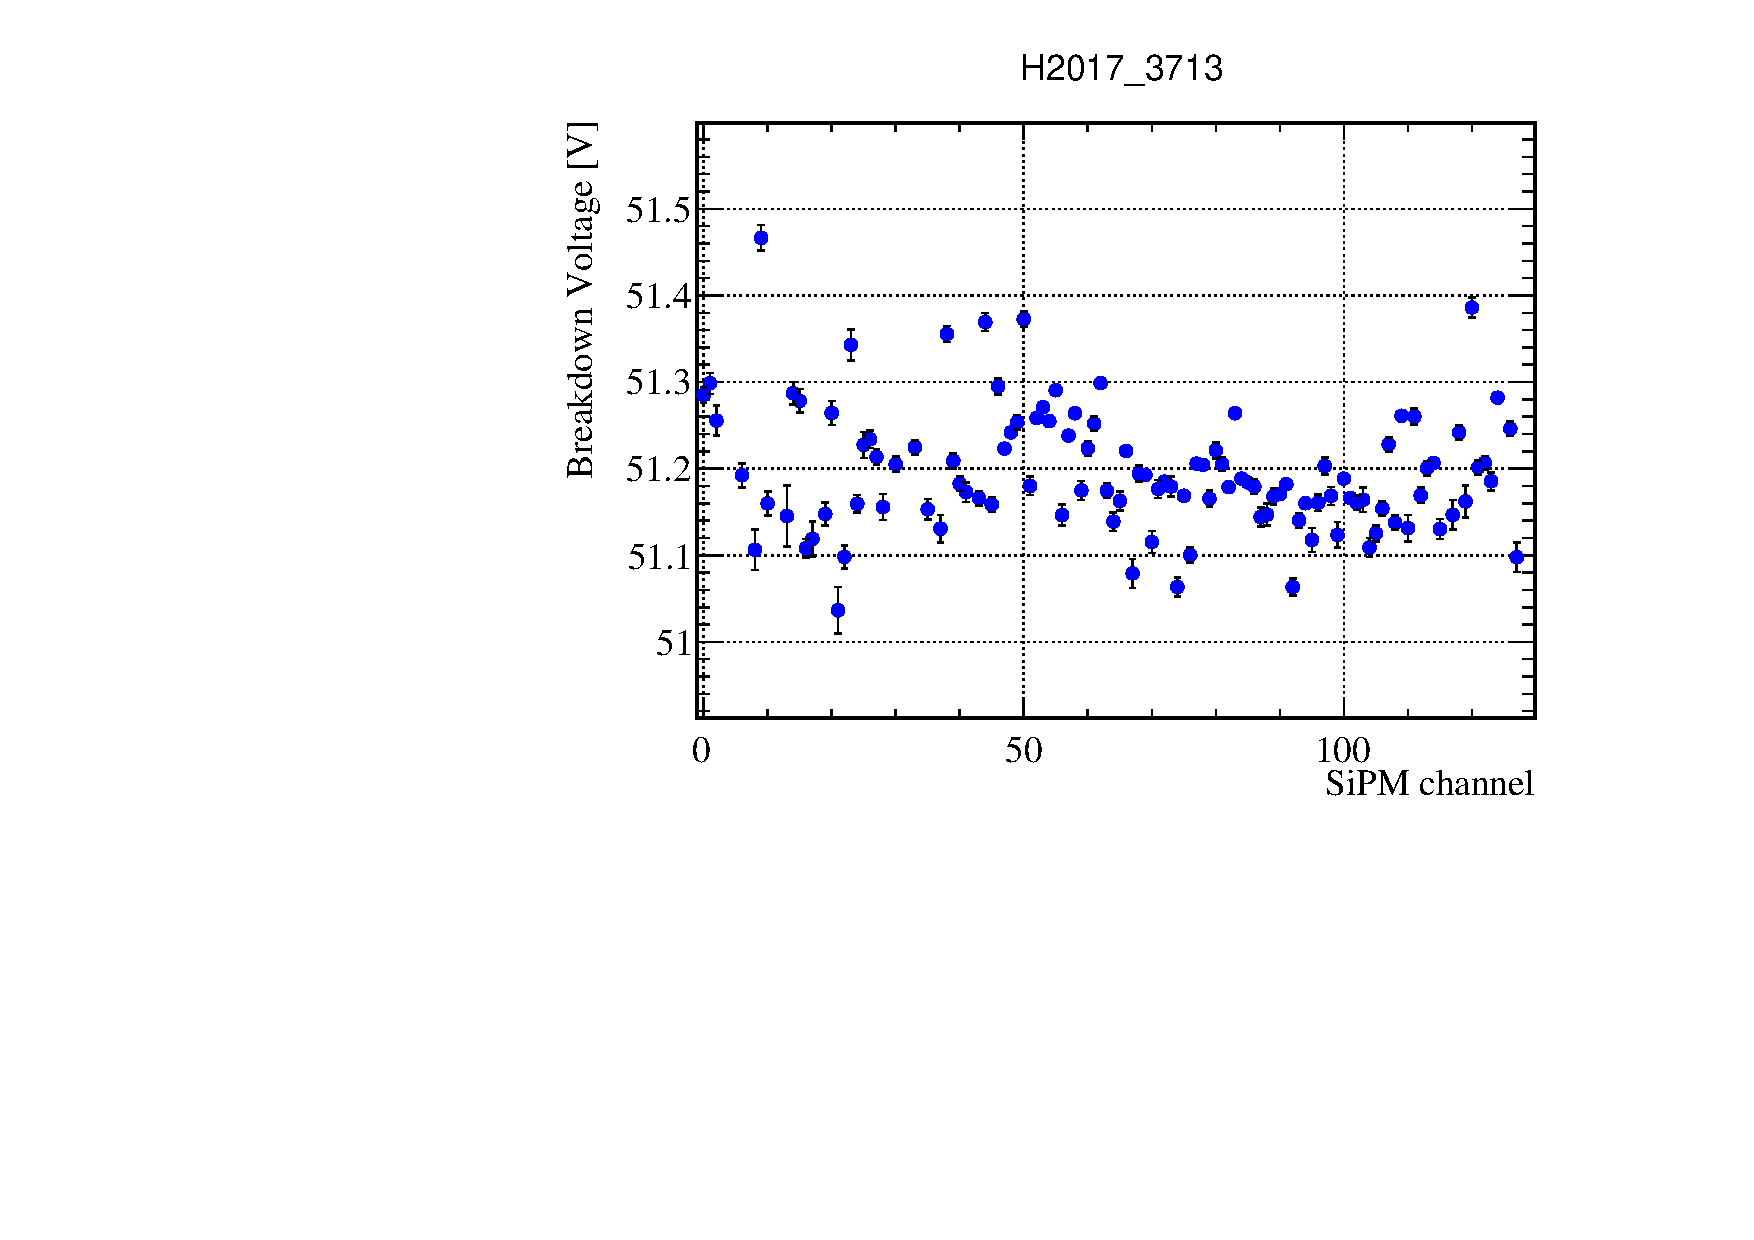
\includegraphics[width=\textwidth]{gfx/plots/WA/H2017/H2016_va64.pdf}
    \caption{$V_{bd}$ H2017.}
    \label{fig:}
  \end{subfigure}
  \caption{Plots of the $V_{bd}$ for all channels (\textbf{VATA64}) for the FBK detectors. }
  \label{fig:Vbd all channels Guido}
\end{figure}

\begin{table}[htbp]
\centering
\begin{tabular}{|c|cc|c|cc|}
\hline
                 & FBK \SI{16}{\micro m}                     & $V_{bd}$ [V] &                  & FBK \SI{31}{\micro m}                    & $V_{bd}$ [V] \\ \cline{2-3} \cline{5-6} 
\textbf{channel} & \multicolumn{1}{c|}{\textbf{WA}} & \textbf{VATA64}  & \textbf{channel} & \multicolumn{1}{c|}{\textbf{WA}} & \textbf{VATA64}  \\ \cline{2-3} \cline{5-6} 
\textbf{70}      & $30.6 \pm 0.3$     & $30.8\pm0.3$   & \textbf{6}       & $30.9\pm0.2$       & $30.9\pm 0.2$     \\
\textbf{86}      & $30.6\pm0.3$       & $30.7\pm 0.3$     & \textbf{36}      & $31.0\pm 0.2$      & $30.8\pm 0.2$     \\ \hline
\textbf{}        & FBK \SI{42}{\micro m}                    & $V_{bd}$ [V] & \textbf{}        & H2017                            & $V_{bd}$ [V] \\ \cline{2-3} \cline{5-6} 
\textbf{channel} & \multicolumn{1}{c|}{\textbf{WA}} & \textbf{VATA64}  & \textbf{channel} & \multicolumn{1}{c|}{\textbf{WA}} & \textbf{VATA64}  \\ \cline{2-3} \cline{5-6} 
\textbf{22}      & $30.9\pm 0.2$      & $31.1\pm 0.2$     & \textbf{54}      & $51.0 \pm 0.2$     &  $51.2\pm 0.2$            \\
\textbf{102}     & $31.0\pm 0.2$      & $31.1 \pm 0.2$      & \textbf{86}      & $51.0 \pm 0.2 $    &  $51.2\pm 0.2$            \\ \hline
\end{tabular}
\caption{$V_{bd}$ corrected with the temperature at \SI{25.0}{\celsius}.}
\label{table:Vbds temp adjusted}
\end{table}

%discussion 

As explained in section \ref{ch:background}, the breakdown voltage value varies from a channel to another and changes as a function of temperature. 
For the WA method, the temperature changed during the measurement. The air conditioner in the lab managed to start the measurement at \SI{25.0}{\celsius} but as overvoltage increases, so did the temperature (up to $26.0-26.5 ^\circ$C). Since this increase of temperature happens for each detectors and at the same amplitudes, the averaged temperature during the measurement is \SI{25.75}{\celsius}. One can then compute the correction associated to this temperature to have the results at \SI{25.0}{\celsius}. As section \ref{ch:background:SiPM:characterised detectors:FBKvsH} tells, the temperature dependency on $V_{bd}$ for the FBK detectors is \SI{32}{\milli V \per \celsius} and \SI{54}{\milli V \per \celsius} for the Hamamatsu. \\
\\
The plots shown in Fig. \ref{fig:Vbd all channels Guido} represent the measured value of $V_{bd}$ for all the channels. The spread in $V_{bd}$ is measured to be $ 0.26$ V, $0.27$V and $0.15$ V for the \SI{16}{\micro m}, \SI{31}{\micro m} and \SI{42}{\micro m} respectively. During the measurement (VATA64), the temperature for the \SI{16}{\micro m} and \SI{31}{\micro m} was \SI{24.7}{\celsius}n \SI{24.6}{\celsius} for the \SI{42}{\micro m} and \SI{25.0}{\celsius} for H2017. 
%The temperature adjustment is then  \SI{9.6}{\milli V} and \SI{12.8}{\milli V} respectively.
These measurements were done by Guido Haefeli and are used as comparison. The measured values (\textbf{WA}) show satisfying results limiting the difference with the \textbf{VATA64} method by less than \SI{200}{\milli V}. 

\section{Noise Classification}
\label{ch:Results:Noise Classification}
% intro 
Finding the correlated noise is necessary to characterize the SiPM. It allows for each detectors to define their operation range and helps in the computation of PDE and gain. Knowing the percentage of DiXT helps to correct measured quantities such as photo-current since DiXT peaks produce more photo-current than a 1 \ac{PE} pulse. But also AP and secondary peaks play a role in the current correction.
The measurement presented in Fig. \ref{fig:correlated noises + epoxy} shows the correlated noise as a function of overvoltage $\Delta V$ for the four FBK detectors, the Hamamatsu H2017. 
\\
The thresholds for classifying the different types of noise have been defined for the H2017, \SI{31}{\micro m} are available on Table \ref{table:thresholds wa}. \SI{16}{\micro m} has the exact same parameters except that the DeXT minimal time is \SI{15.0}{\nano s}. For the \SI{42}{\micro m}, the only change is AP [$ 0.5$, $ 0.85 $[. \SI{31}{\micro m} + epoxy detector had a lot of ringing  and secondary peaks making the classification difficult. To avoid an over correction of the PDE, the DiXT time threshold was increased to \SI{20}{\nano s} and the DeXT amplitude to \SI{0.9}{PE}.

\begin{table}[htbp]
\centering
\begin{tabular}{|c|c|c|c|}
\hline
\textbf{Threshold}      & \textbf{DiXT} & \textbf{DeXT}   & \textbf{AP}     \\ \hline
\textbf{Time [ns]}      & $\leq2.0$     & >$2.0$          & >$15.0$         \\ \hline
\textbf{Amplitude [PE]} & >$1.17$       & ]$ 0.85 $,$ 1.17 $] & [$ 0.6 $, $ 0.85 $[ \\ \hline
\end{tabular}
\caption{Thresholds for the noise classification.}
\label{table:thresholds wa}
\end{table}

To cross check that the thresholds are tuned properly, one can plot the waveform maximal amplitude as a function of their arrival time as in Fig. \ref{fig:peakamptime 42} for the \SI{42}{\micro m}: One can see the different noises, including secondaries than may be just due to misidentification.

\newgeometry{left=1.5cm,right=1.5cm,top=2cm,bottom=2cm}
\begin{figure}[htbp]
  \centering
  \begin{subfigure}{0.48\textwidth}
    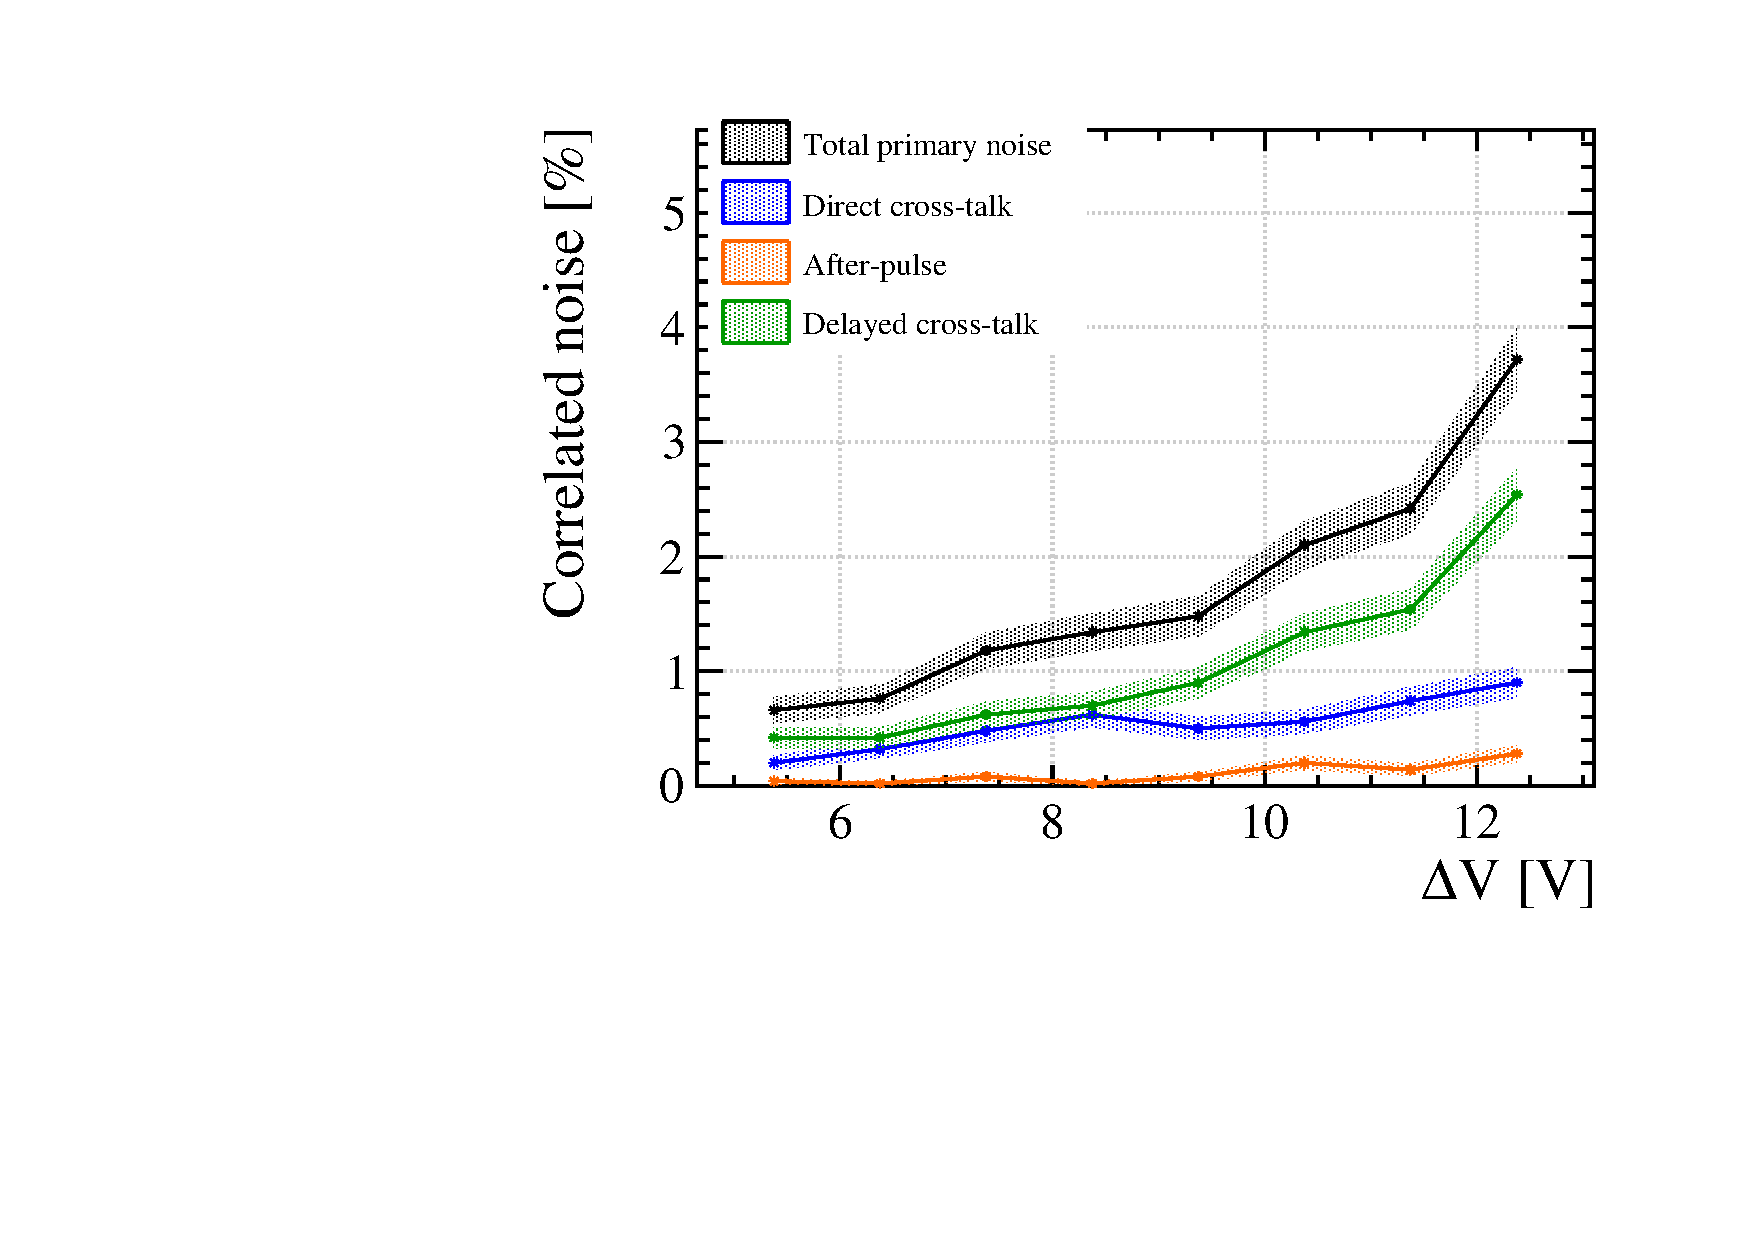
\includegraphics[width=1\linewidth]{gfx/plots/WA/16/CorrelatedNoise.pdf}
    \caption{FBK \SI{16}{\micro m}, channel $70$.}
    \label{fig:}
  \end{subfigure}
  \hfill
  \begin{subfigure}{0.48\textwidth}
    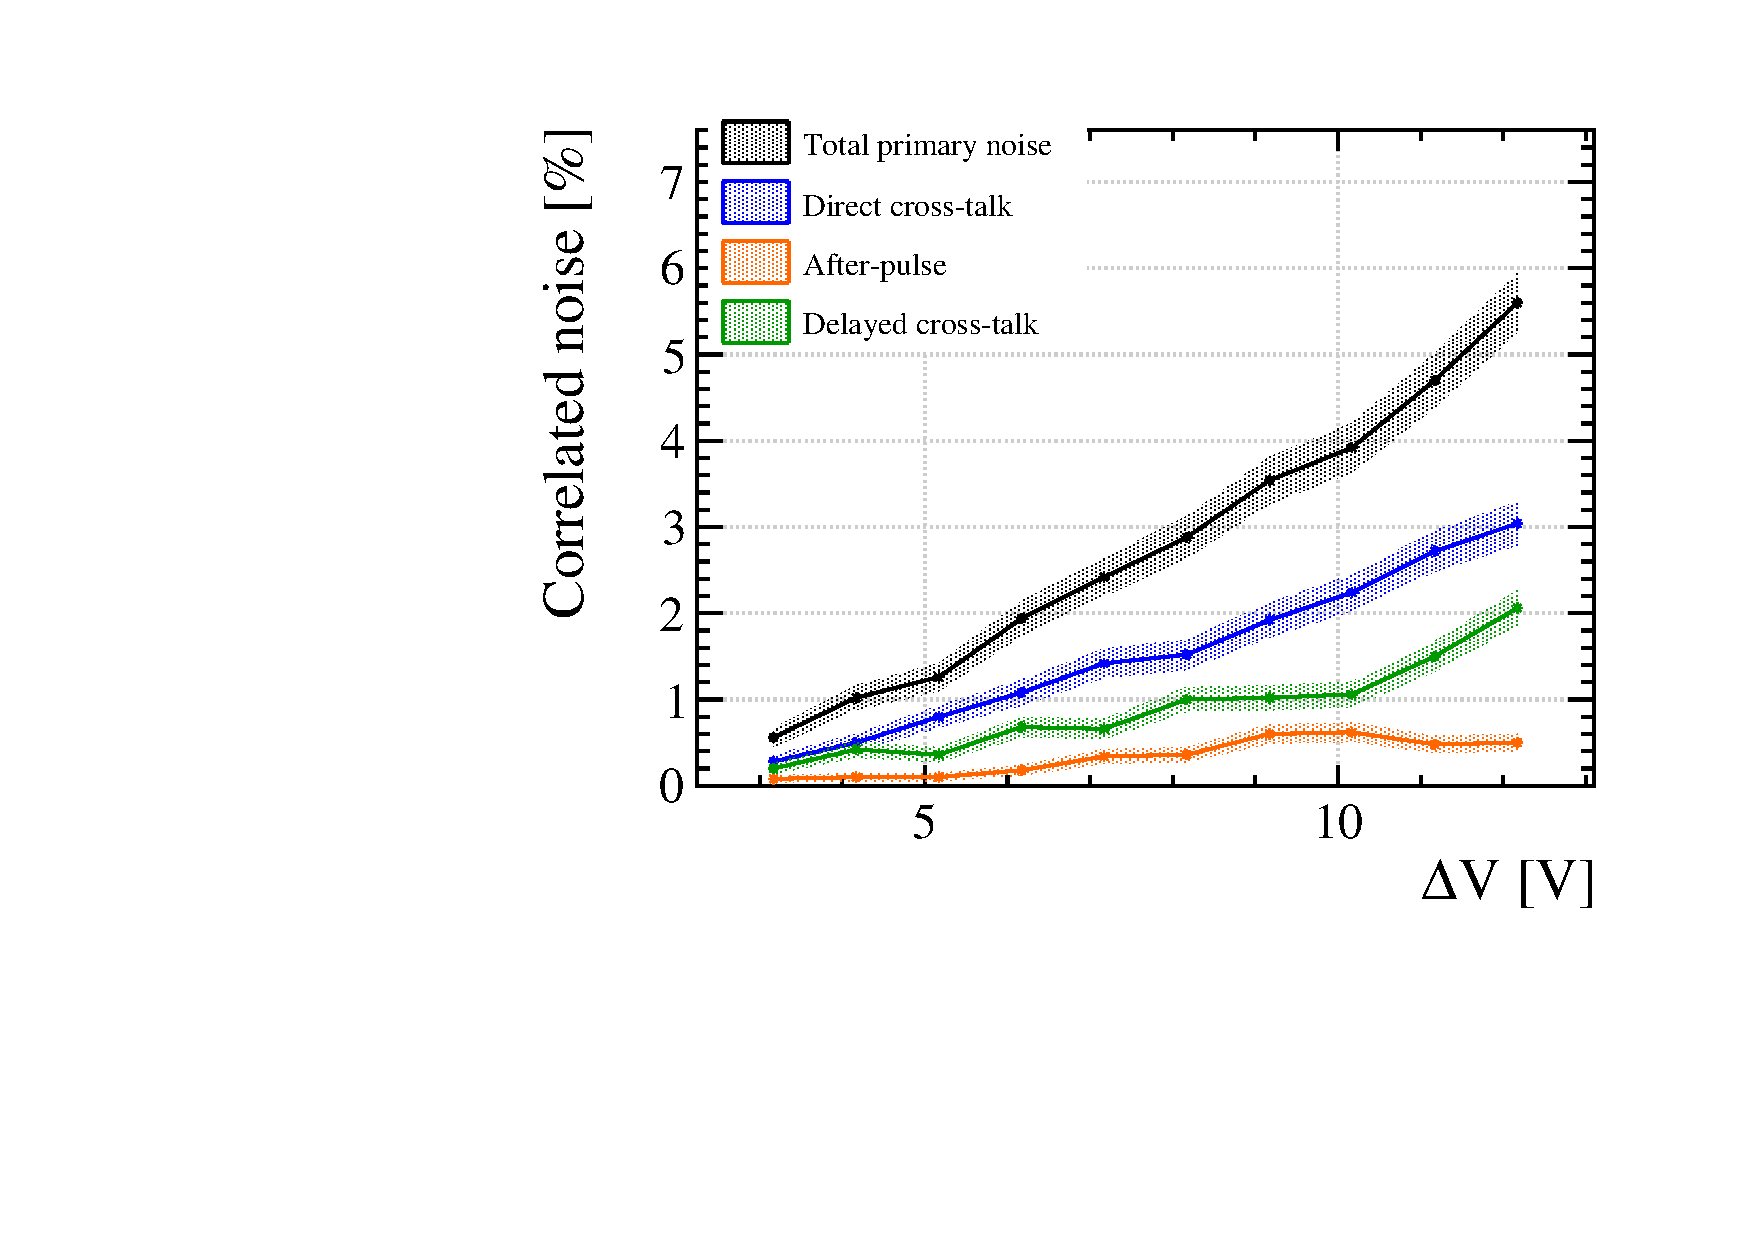
\includegraphics[width=1\linewidth]{gfx/plots/WA/31/CorrelatedNoise.pdf}
    \caption{FBK \SI{31}{\micro m}, channel $86$.}
    \label{fig:}
  \end{subfigure}
  \hfill
  \begin{subfigure}{0.48\textwidth}
    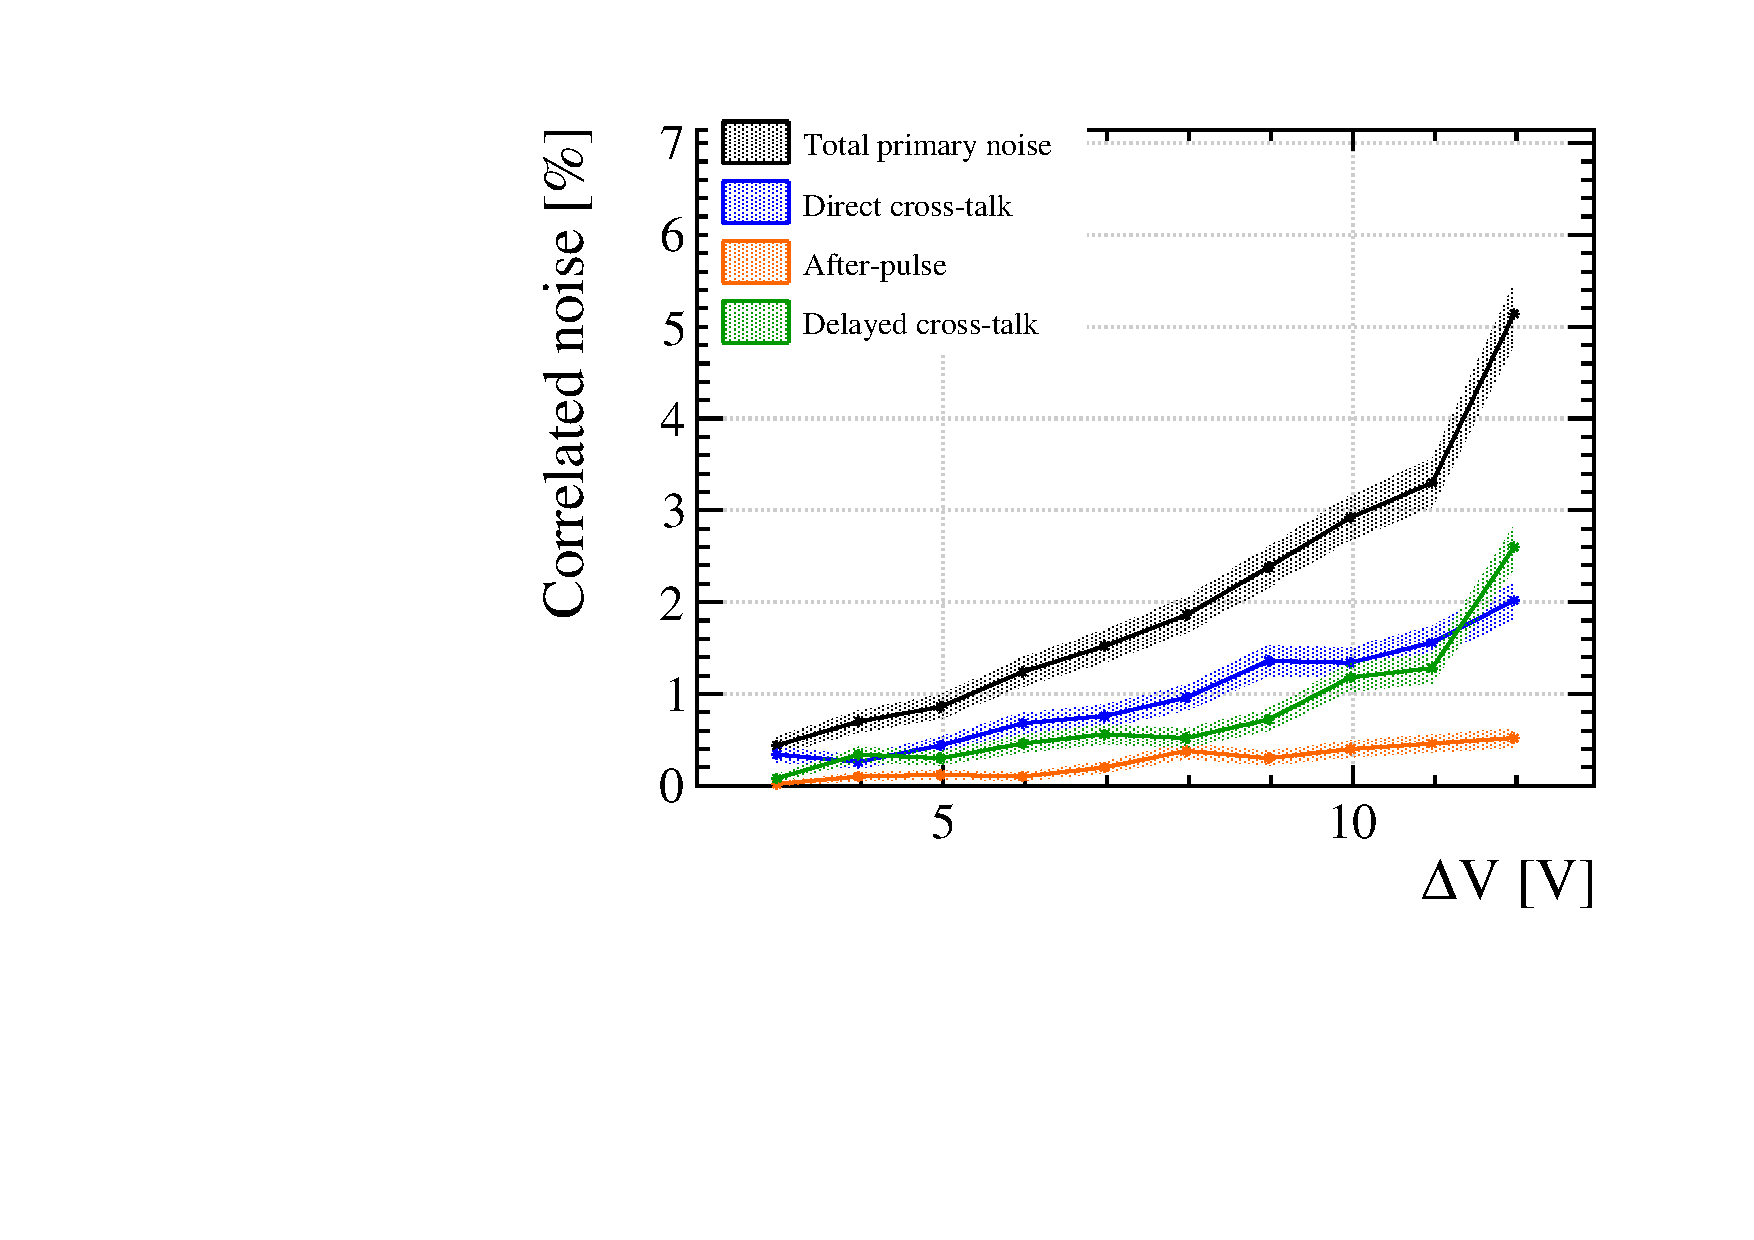
\includegraphics[width=1\linewidth]{gfx/plots/WA/42/CorrelatedNoise.pdf}
    \caption{FBK \SI{42}{\micro m}, channel $54$.}
    \label{fig:}
  \end{subfigure}
  \hfill
   \begin{subfigure}{0.48\textwidth}
    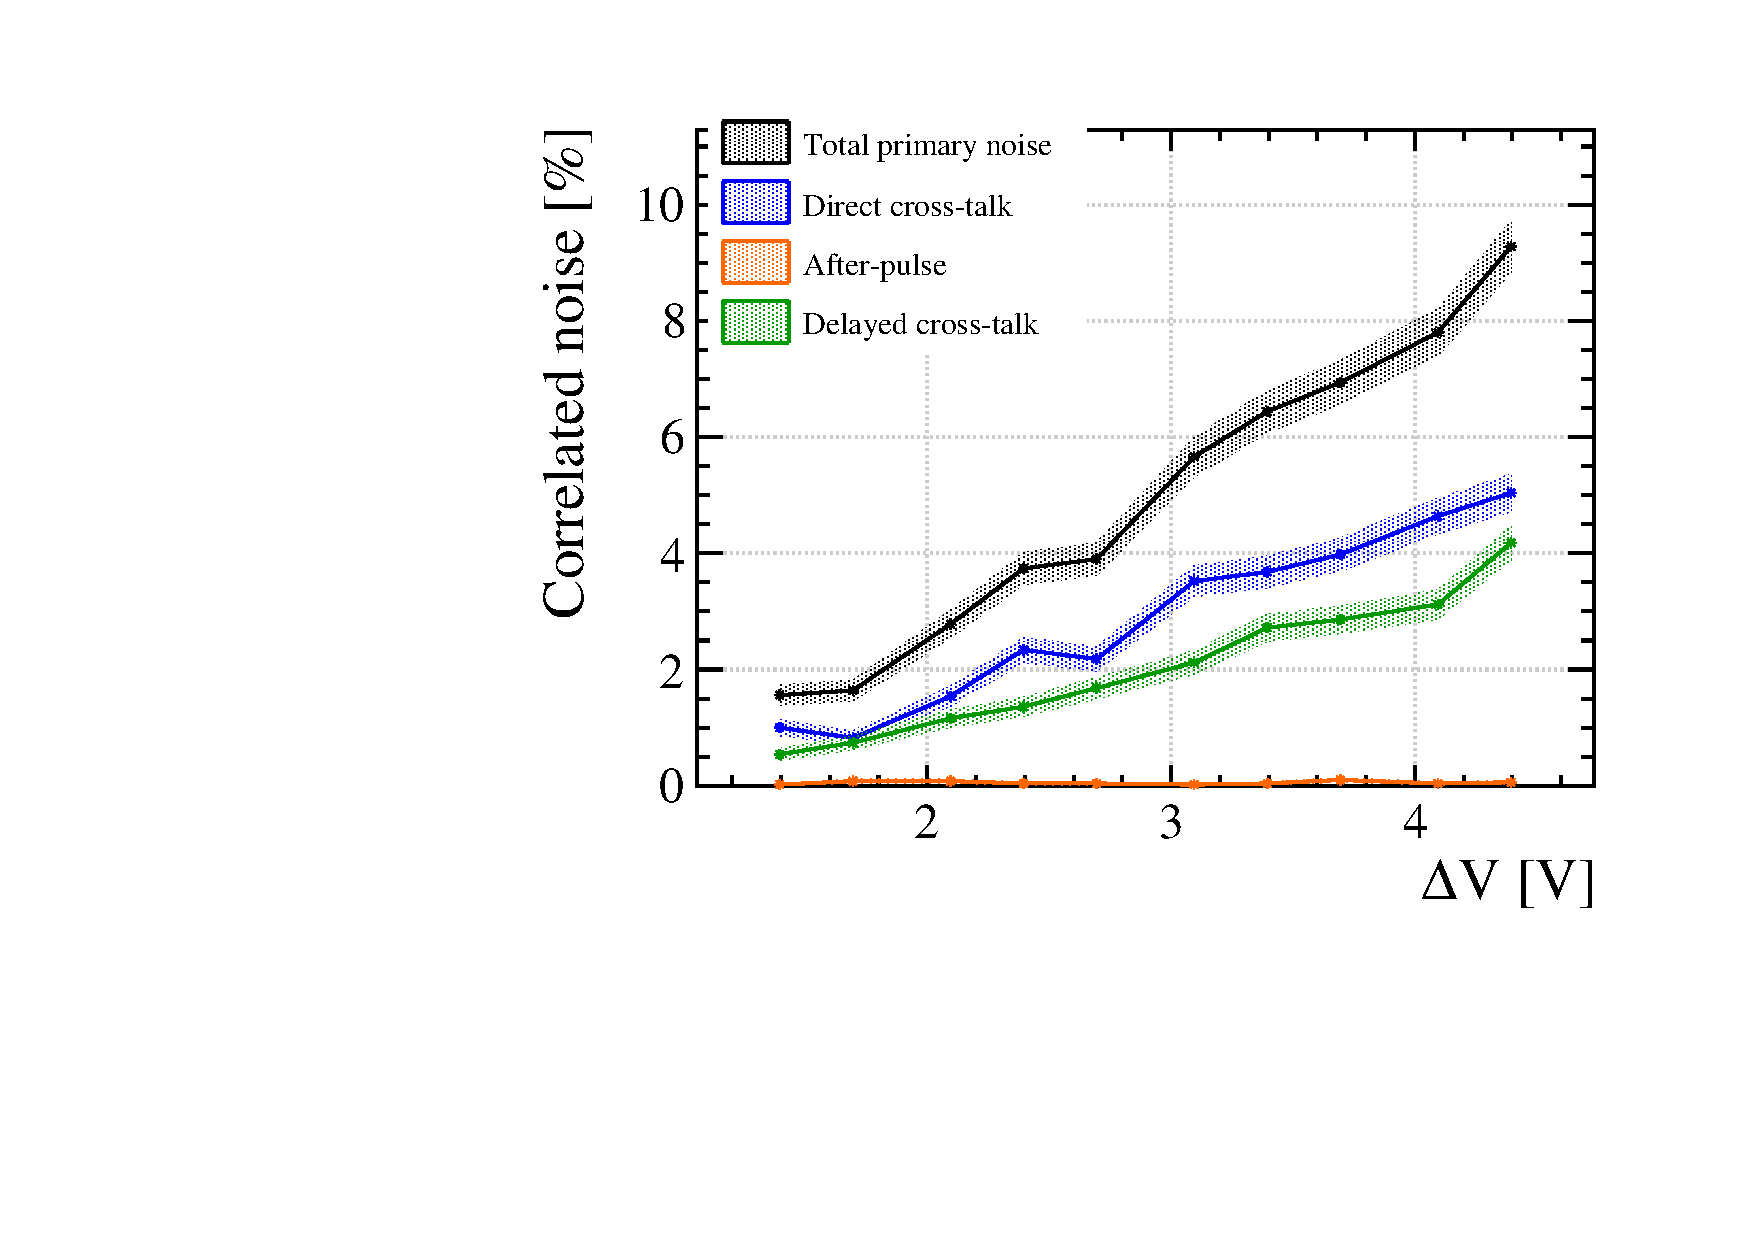
\includegraphics[width=1\linewidth]{gfx/plots/WA/H2017/CorrelatedNoise.pdf}
    \caption{H2017, channel $54$.}
  \end{subfigure}
  \hfill
   \begin{subfigure}{0.48\textwidth}
    \includegraphics[width=1\linewidth]{gfx/plots/WA/31epoxy/CorrelatedNoise.pdf}
    \caption{FBK \SI{31}{\micro m} + epoxy, channel $22$.}
  \end{subfigure}
\caption{Correlated noise of the FBK \SI{16}{\micro m} (a), \SI{31}{\micro m} (b), \SI{42}{\micro m} (c), H2017 (d) and FBK \SI{31}{\micro m} + epoxy layer (e) SiPM. }
\label{fig:correlated noises + epoxy}
\end{figure}

\begin{figure}[htbp]
    \centering
       \begin{subfigure}{0.48\textwidth}
        \includegraphics[width=1\linewidth]{gfx/plots/WA/16/clwf16.pdf}
        \caption{}
      \end{subfigure}
      \hfill
       \begin{subfigure}{0.48\textwidth}
        \includegraphics[width=1\linewidth]{gfx/plots/WA/31/clwf31.pdf}
        \caption{}
      \end{subfigure}
      \hfill
       \begin{subfigure}{0.48\textwidth}
        \includegraphics[width=1\linewidth]{gfx/plots/WA/42/clwf42.pdf}
        \caption{}
      \end{subfigure}
      \hfill
       \begin{subfigure}{0.48\textwidth}
        \includegraphics[width=1\linewidth]{gfx/plots/WA/H2017/clwfh2017.pdf}
        \caption{}
      \end{subfigure}
    \caption{Clean waveforms for the FBK \SI{16}{\micro m} (a), \SI{31}{\micro m} (b), \SI{42}{\micro m} (c) and Hamamatsu H2017 (d).}
    \label{fig:pulse shape clean waveforms}
\end{figure}

\restoregeometry

\begin{figure}[htbp]
    \centering
    \begin{subfigure}{0.7\textwidth}
        \includegraphics[width=\textwidth]{gfx/plots/WA/DiXTs_wo_epoxy.pdf}
        \caption{}
    \end{subfigure}
    \hfill
    \begin{subfigure}{0.7\textwidth}
        \includegraphics[width=\textwidth]{gfx/plots/WA/DiXTs.pdf}
        \caption{}
    \end{subfigure} 
    \caption{DiXT for the different four studied detectors (a) and with the \SI{31}{\micro m} with the epoxy layer (b).}
    \label{fig:DiXT detectors}
\end{figure}


% fbk and hamamatsu
The first observation one can make about the FBK detectors is their very low correlated noise even at high overvoltage. At $\Delta V= 12$ V, the FBK have $4\%$ to $6\%$ of total correlated noise. The Hamamatsu cannot operate in this region, but at its maximal operation range (around $\Delta V= 5$ V), the Hamamatsu is at $\approx 9.5\%$ of total correlated noise. At this $\Delta V$ the FBK detectors have $8$ to $12$ times less correlated noise. Having a higher operation range without increasing the correlated noise helps in improving the PDE. This difference is highlighted by Fig. \ref{fig:DiXT detectors} (a) where the DiXT is very low the for the FBK detectors. Operating at high PDE reduces the errors on $V_{bd}$ since we work in wider operation range. 
\\
The FBK \SI{16}{\micro m} has more DeXT than DiXT, which is not the case for the two other detectors from FBK. This may be due to a misidentification between direct and delayed cross talk. The pulse shapes for the four detectors are very different, and shown in Fig. \ref{fig:pulse shape clean waveforms}. One can see on the \SI{16}{\micro m} (a) that one signal is misidentified as 'clean' (in pale blue). Also, since the pixel sizes are smaller for the \SI{16}{\micro m} and \SI{31}{\micro m}, the signal amplitude is also smaller resulting in a lower signal to noise ratio. It is clearly visible on Fig. \ref{fig:pulse shape clean waveforms} (a) \& (b) where the baseline is way thicker than for the bigger pixel sizes (c) \& (d).\\ 
%31um epoxy talk 
\\
An interesting comparison between the FBK \SI{31}{\micro m} and its version with the epoxy layer can be done. Correlated noise plots are shown in Fig. \ref{fig:correlated noises + epoxy} (b) \& (e) respectively. The addition of an epoxy layer increases the total correlated noise by a factor of $6$ for all the overvoltage range. This result is explained by the fact that most of the noise comes from external cross talk. The photons issued from an avalanche by bremsstrahlung may be reflected by the epoxy layer, allowing this photon to hit another neighbour pixel causing external cross talk. Delayed cross talk is also increased.

%\begin{table}[]
%\begin{tabular}{|c|c|c|c|c|}
%\hline
%Detector                            & FBK \SI{16}{\micro m}   & FBK \SI{31}{\micro m} & FBK \SI{42}{\micro m} & H2017         \\ \hline
%Operation range$\cdot \Delta V$ [V] & [$5.4$-$12.4$] & [$3$-$12$]   & [$3$-$12$]   & [$0.8$-$4.6$] \\ \hline
%\end{tabular}
%\caption{Operation range for the studied detectors.}
%\label{table:operation ranges}
%\end{table}

\section{Gain}
\label{ch:Results:Gain}


The gain results are shown in Fig. \ref{fig:Gain fit for all detectors} and presented per unit of overvoltage.

Difficulties in the measurements have been encountered especially at low operation voltages for the FBK detectors. As explained in section \ref{ch:Results:Noise Classification}, the noise is very present at low $\Delta V$ for small pixel size (smaller pulse amplitude). 

\begin{figure}[htbp]
    \centering
    \includegraphics[width=0.8\textwidth]{gfx/plots/Gain/Gain(pixel size)_area.pdf}
    \caption{Relation between the gain and the pixel active area.}
    \label{fig:gain(area)}
\end{figure}


The first observation is that the measured value for the Hamamatsu H2017 matches with \cite{Girard2018CharacterisationDistributions}. 
\\
The smaller the pixel size, the smaller the gain. This is confirmed by the measurement where the FBK \SI{16}{\micro m} has the smallest gain value, followed by the \SI{31}{\micro m} and then \SI{42}{\micro m}. The reason why the gain depends on the pixel size is purely physical; the more active area (hence pixel size), the more electron-hole pair will be created during the avalanche and hence more current is produced. 
An interesting comparison is shown in Fig. \ref{fig:gain(area)}. Here, the gain as a function of the active area. Ideally, it would be a good choice to represent the gain as a function of the total active volume, but the thickness of the layers is not known. The surface plot is still valid at first approximation since the 3 samples from FBK analyzed are from the same wafer (W1). The thickness of the sample vary only due to some disparities but the process of adding the thin layers is considered homogeneous. A linear relation is clearly visible on Fig. \ref{fig:gain(area)} and confirms the gain dependency to the active volume. The Hamamatsu is shown as comparison and of course do not have the same dependency since it is not the same technology, wafer and process of fabrication. \\
\\
These gain measurements also provide inputs on the $V_{bd}$, the $V_{offset}$ represents the difference between $V_{bd,WA}$ from the waveform analysis and $V_{bd,G}$ by quantifying this difference at the extrapolation to zero of the fit. Significant differences from \SI{-0.8}{\volt} to \SI{+0.3}{\volt} showed that the $V_{WA,bd}$ may not be accurate enough especially for the H2017 where the gain is well fitted. Nevertheless, the gain measurement of the FBK are less precise, and we will see later \ref{ch:Results:PDE} that is has less influence on the PDE. 

\newgeometry{left=0.8cm,right=0.8cm,top=2cm,bottom=2cm}

\begin{figure}[htbp]
  \centering
  \begin{subfigure}{0.48\textwidth}
    \includegraphics[width=\textwidth]{gfx/plots/Gain/16/Gain.pdf}
    \caption{FBK \SI{16}{\micro m}, channel $70$.}
    \label{fig:16 gain}
  \end{subfigure}
  \hfill
  \begin{subfigure}{0.48\textwidth}
    \includegraphics[width=\textwidth]{gfx/plots/Gain/31/Gain.pdf}
    \caption{FBK \SI{31}{\micro m}, channel $86$.}
    \label{fig:31 gain}
  \end{subfigure}
    \begin{subfigure}{0.48\textwidth}
    \includegraphics[width=\textwidth]{gfx/plots/Gain/42/Gain.pdf}
    \caption{FBK \SI{42}{\micro m}, channel $22$.}
    \label{fig:42 gain }
  \end{subfigure}
  \hfill
  \begin{subfigure}{0.48\textwidth}
    \includegraphics[width=\textwidth]{gfx/plots/Gain/H2017/Gain.pdf}
    \caption{H2017, channel $70$.}
    \label{fig:H2017 gain }
  \end{subfigure}
  \hfill
  \begin{subfigure}{0.48\textwidth}
    \includegraphics[width=\textwidth]{gfx/plots/Gain/31epoxy/Gain.pdf}
    \caption{FBK \SI{31}{\micro m}+ epoxy , channel $54$.}
    \label{fig:31 epoxy gain}
  \end{subfigure}
  \hfill
  \caption{Plots of the gain fit for all the studied detectors. }
  \label{fig:Gain fit for all detectors}
\end{figure}

\restoregeometry


\section{Photo-detection efficiency}
\label{ch:Results:PDE}
The PDE is measured as a function of both overvoltages and wavelengths. Measurements for $10$ different overvoltages and $50$ wavelength are performed. The PDE for the FBK \SI{16}{\micro m}, \SI{31}{\micro m}, \SI{42}{\micro m} and Hamamatsu H2017 are in Fig. \ref{fig:pde 16um}, Fig. \ref{fig:pde 31um}, Fig. \ref{fig:pde 42um} and \ref{fig:pde H2017} respectively. The PDE of the the \SI{31}{\micro m} with an epoxy layer is shown in \ref{fig:pde 31epoxy}.
On Fig. \ref{fig:pde comp epoxy} is shown for one wavelength (a) the PDE as a function of overvoltage and for one $\Delta V = 10.02$ V (b), the PDE as a function of $\lambda$ for the \SI{31}{\micro m} with and without the epoxy coating. \\
\\
The current method needs the gain measurement and then more errors are induced by this method compared to the rate. 
Is it observed that the current method underestimate the PDE relatively to the rate method by $2\%$ to $8.5\%$ of the rate PDE value at $\Delta V=12 $ V for the FBK. The maximal difference is in the \SI{42}{\micro m}. \\
\\
For the FBK bare die detectors, one can see the PDE oscillating as $\lambda$ increases. The amplitude of these oscillations is around $5\%$ of the absolute PDE value. 
One explication possible for these oscillations could be explained by optical interference in the \ac{ARC} on top of the detector. Reflected photons within the media layer could interfere constructively and destructively resulting in oscillations of the PDE. 
\\
% PDE as delta V 
As predicted by the theory, increasing the overvoltage increases the PDE but only in the operation range. Beyond, it saturates and stops increasing. This is another way of defining the operation range of the detectors. Some figures showed a decrease of the PDE by $2\%$ but this could be explained by an over correction of the noise, especially at low overvoltage where the errors in the correlated noise are bigger. 
%of a detectors and the result shown in Table. \ref{table:operation ranges}, can be confirmed or refined.
\\
%The peak sensitivity wavelength is measured of $\lambda_p = 475$nm for both current and frequency methods, which is similar to the measured $\lambda_p \approx 480$nm in \cite{Girard2018CharacterisationDistributions}. There is still a difference compared to the announced value of $450$ nm \cite{SurfaceArray}.
\\
% H2017 comparison 
Results for the Hamamatsu H2017 are shown in Fig. \ref{fig:pde H2017} and match with the measurement in  especially at high overvoltage \cite{Girard2018CharacterisationDistributions}. Some differences are noticeable, if we look at $\Delta V = 3.5$V, the maximal PDE value in \cite{Girard2018CharacterisationDistributions} is $44 \%$ whereas in \ref{fig:pde H2017}, it reaches $38\%$.
The PIN Diode calibration is a major cause of uncertainties due to errors on the calibration, also the light diffuser is not the same as in \cite{Girard2018CharacterisationDistributions}. Following this, we have not pursued these calibration uncertainties since what concerns us  for R\&D is more the differences of PDE between FBK and Hamamatsu. 
Another hint on these differences could be due the oscilloscope which has a lower band with than in \cite{Girard2018CharacterisationDistributions}. A \SI{300}{\milli V} error on $V_{bd}$ could shift the overvoltage axis (on the PDE$(\Delta V)$ plots) such that the absolute PDE value changes by several points ($1$ to $3\%$). This error is not visible on the FBK because the relative error on $V_{bd}$ is reduce due to the higher operation range.\\
\\
% epoxy talk 
In the SciFi tracker, the detectors will be installed at the output of the fibres. Since the FBK have been studied bare die, another sample of the \SI{31}{\micro m} was studied with an epoxy layer as additional coating. The results on the PDE are visible on Fig. \ref{fig:pde 31epoxy} and one can clearly see that the oscillations are cancelled. %The peak sensitivity for the FBK NUV-HD is announced around $\lambda_p= 400$nm \cite{} and the measurement are partially in agreement with this, even though measurement below $400$nm should be done to confirm it. Nevertheless, since the light coming from the SciFi is not below $400$nm, this information is not relevant for us. 
One can notice on the plots of the PDE as a function of $\Delta V$ (left plot) that at very high $\Delta V$, the efficiency saturates reaching a maximal value of $45\%$ at $\Delta V=12 $ V. The comparison with the bare die detector and with the epoxy layer for one overvoltage is shown in Fig. \ref{fig:pde comp epoxy}. We notice that the epoxy version behaves as the mean value of the oscillations. 
% general comments about SiPMs
It is observed that the detectors with smaller pixels has a smaller PDE because of their lower FF. 

\newgeometry{left=0.5cm,right=0.5cm,top=1.5cm,bottom=1.5cm}
\begin{landscape}
\begin{figure}[htbp]
    \centering
    \begin{subfigure}{0.65\textwidth}
        \includegraphics[width=\linewidth]{gfx/plots/PDE/16/c_Current_Bias.pdf}  
        \caption{Current}
    \end{subfigure}
    %\hfill
    \begin{subfigure}{0.65\textwidth}
        \includegraphics[width=\linewidth]{gfx/plots/PDE/16/c_Current_Wavelength.pdf}  
        \caption{Current}
    \end{subfigure}
    \\
    \begin{subfigure}{0.65\textwidth}
        \includegraphics[width=\linewidth]{gfx/plots/PDE/16/c_Freq_Bias.pdf}    
        \caption{Rate}
    \end{subfigure}
    %\hfill
    \begin{subfigure}{0.65\textwidth}
        \includegraphics[width=\linewidth]{gfx/plots/PDE/16/c_Freq_Wavelength.pdf} 
        \caption{Rate}
    \end{subfigure}
    \caption{PDE of the FBK \SI{16}{\micro m}.}
    \label{fig:pde 16um}
\end{figure}

\end{landscape}

\begin{landscape}
\begin{figure}[htbp]
    \centering
    \begin{subfigure}{0.65\textwidth}
        \includegraphics[width=\linewidth]{gfx/plots/PDE/31/c_Current_Bias.pdf}  
        \caption{Current}
    \end{subfigure}
    %\hfill
    \begin{subfigure}{0.65\textwidth}
        \includegraphics[width=\linewidth]{gfx/plots/PDE/31/c_Current_Wavelength.pdf}  
        \caption{Current}
    \end{subfigure}
    \\
    \begin{subfigure}{0.65\textwidth}
        \includegraphics[width=\linewidth]{gfx/plots/PDE/31/c_Freq_Bias.pdf}    
        \caption{Rate}
    \end{subfigure}
    %\hfill
    \begin{subfigure}{0.65\textwidth}
        \includegraphics[width=\linewidth]{gfx/plots/PDE/31/c_Freq_Wavelength.pdf} 
        \caption{Rate}
    \end{subfigure}
    \caption{PDE of the FBK \SI{31}{\micro m}.}
    \label{fig:pde 31um}
\end{figure}
\end{landscape}

\begin{landscape}  
\begin{figure}[htbp]
    \centering
    \begin{subfigure}{0.65\textwidth}
        \includegraphics[width=\linewidth]{gfx/plots/PDE/42/c_Current_Bias.pdf}  
        \caption{Current}
    \end{subfigure}
    %\hfill
    \begin{subfigure}{0.65\textwidth}
        \includegraphics[width=\linewidth]{gfx/plots/PDE/42/c_Current_Wavelength.pdf}  
        \caption{Current}
    \end{subfigure}
    \\
    \begin{subfigure}{0.65\textwidth}
        \includegraphics[width=\linewidth]{gfx/plots/PDE/42/c_Freq_Bias.pdf}    
        \caption{Rate}
    \end{subfigure}
    %\hfill
    \begin{subfigure}{0.65\textwidth}
        \includegraphics[width=\linewidth]{gfx/plots/PDE/42/c_Freq_Wavelength.pdf} 
        \caption{Rate}
    \end{subfigure}
    \caption{PDE of the FBK \SI{42}{\micro m}. }
    \label{fig:pde 42um}
\end{figure}
\end{landscape}

\begin{landscape}
\begin{figure}[htbp]
    \centering
    \begin{subfigure}{0.65\textwidth}
        \includegraphics[width=\linewidth]{gfx/plots/PDE/H2017/c_Current_Bias.pdf} 
        \caption{Current}
    \end{subfigure}
    %\hfill
    \begin{subfigure}{0.65\textwidth}
        \includegraphics[width=\linewidth]{gfx/plots/PDE/H2017/c_Current_Wavelength.pdf}  
        \caption{Current}
    \end{subfigure}
    \\
    \begin{subfigure}{0.65\textwidth}
        \includegraphics[width=\linewidth]{gfx/plots/PDE/H2017/c_Freq_Bias.pdf}    
        \caption{Rate}
    \end{subfigure}
    %\hfill
    \begin{subfigure}{0.65\textwidth}
        \includegraphics[width=\linewidth]{gfx/plots/PDE/H2017/c_Freq_Wavelength.pdf} 
        \caption{Rate}
    \end{subfigure}
    \caption{PDE of the Hamamatsu H2017.}
    \label{fig:pde H2017}
\end{figure}
\end{landscape}

\begin{landscape}
\begin{figure}[htbp]
    \centering
    \begin{subfigure}{0.65\textwidth}
        \includegraphics[width=\linewidth]{gfx/plots/PDE/31epoxy/c_Current_Bias.pdf}  
        \caption{Current}
    \end{subfigure}
    %\hfill
    \begin{subfigure}{0.65\textwidth}
        \includegraphics[width=\linewidth]{gfx/plots/PDE/31epoxy/c_Current_Wavelength.pdf}  
        \caption{Current}
    \end{subfigure}
    \\
    \begin{subfigure}{0.65\textwidth}
        \includegraphics[width=\linewidth]{gfx/plots/PDE/31epoxy/c_Freq_Bias.pdf}    
        \caption{Rate}
    \end{subfigure}
    %\hfill
    \begin{subfigure}{0.65\textwidth}
        \includegraphics[width=\linewidth]{gfx/plots/PDE/31epoxy/c_Freq_Wavelength.pdf} 
        \caption{Rate}
    \end{subfigure}
    \caption{PDE of the FBK \SI{31}{\micro m} + epoxy layer.}
    \label{fig:pde 31epoxy}
\end{figure}
\end{landscape}
\restoregeometry

\begin{figure}[htbp]
    \centering
    \includegraphics[width=0.8\textwidth]{gfx/plots/PDE/PDEcomp.pdf}  
    \caption{PDE of the FBK \SI{31}{\micro m} with and without the epoxy layer at fixed $\Delta V$.}
    \label{fig:pde comp epoxy}
\end{figure}


\chapter{Conclusion}
\label{ch:Conclusion}

This work has been dedicated to characterise the three FBK detectors. Methods already developed in \cite{Girard2018CharacterisationDistributions} have been reproduced with the Hamamatsu H2017 and applied to the FBK SiPMs. \\
Three different experiment setups were employed and used to characterise different properties of the \SI{16}{\micro m}, \SI{31}{\micro m}, \SI{42}{\micro m} SiPM from FBK and the H2017 SiPM from Hamamatsu.
The IV setup provided measurements of the breakdown voltage less accurate than the waveform analysis and was abandoned. Nevertheless, the quenching resistor $R_Q$ has been measured for $16$ channels out of $128$ with acceptable results. A mean $R_Q$ of \SI{550}{\kilo \ohm}, \SI{436}{\kilo \ohm}, \SI{444}{\kilo \ohm}  and \SI{503}{\kilo \ohm} for H2017, \SI{16}{\micro m}, \SI{31}{\micro m} and \SI{42}{\micro m} respectively compared to an announced value of  \SI{500}{\kilo \ohm} for all was measured. The spread is below $5\%$ for the FBK SiPMs and of $7.4\%$ for the Hamamatsu. 
\\

The waveform analysis setup has enabled us to get breakdown voltage values with an accuracy of  \SI{200}{\milli \volt} for all detectors except the FBK \SI{16}{\micro m} (\SI{300}{\milli \volt}). Two channels per detector were analysed and the results were compared with the values with the VATA64 method.  
The correlated noise has also been obtained with the waveform analysis. FBK detectors can operate up to $\Delta V = 12$ V whereas the Hamamatsu is limited to $ \Delta V = 5$V. This increase of operation range is possible because the correlated noise for the FBK detectors is really low:  $(3.8 \pm 0.2)\%$, $(4.6\pm0.3)\%$ and $(5.2\pm0.3)\%$ at $\Delta V = 12$ V for the \SI{16}{\micro m}, \SI{31}{\micro m} and \SI{42}{\micro m} respectively. At $\Delta V = 4$ V the Hamamatsu H2017 has $(7.5\pm 0.3)\%$ of correlated noise which represents $9.3$ times more noise than the FBK \SI{42}{\micro m}. 
%Nevertheless, due to a too little signal at very low overvoltage, the SiPMs with the smallest pixels from FBK cannot operate well below $5 \Delta V$.
\\
%The difference in operation range and correlated noise is very important, 
The PDE and Gain setup coupled to the wave analysis allowed to measure the gain and PDE for each detector. A comparison of the \SI{31}{\micro m} and another \SI{31}{\micro m} with an additional layer of epoxy glue was studied to see its effect on the PDE. 
The gain of the FBK detectors has been measured with $2\%$ errors and values of $(0.142 \pm 3)\cdot10^{6} $V$^{-1}$, $(0.446\pm 0.009)\cdot10^{6} $V$^{-1}$ and $(0.770\pm 0.015)\cdot10^{6} 
$V$^{-1}$ for the \SI{16}{\micro m}, \SI{31}{\micro m} and \SI{42}{\micro m} respectively. The Hamamatsu H2017 gain was the same value as measured in \cite{Girard2018CharacterisationDistributions}, $(1.022\pm 0.02)\cdot10^{6}$V$^{-1}$. These measurements showed the relation between the pixel size and the gain. They are also a way to cross check the $V_{bd}$ value. 
The PDE measurements showed and oscillating behavior of the PDE as the wavelength varied. Reaching a maximum around \SI{410}{\nano m} of $29\%$, $52\%$, $57\%$ for \SI{16}{\micro m} , \SI{31}{\micro m} and \SI{42}{\micro m} at $\Delta V = 12$ V (for the optimal $\Delta V$ and with a $\approx 4\%$ amplitude). The Hamamatsu has at $\lambda \approx 470$ nm a peak PDE of $40\%$ at $\Delta V = 4.4$ V.
Adding an epoxy layer on the FBK \SI{31}{\micro m} cancelled the oscillations and reduced the PDE by $10\%$ of the \SI{31}{\micro m} bare die with a peak efficiency at measured $46\%$ at $\Delta V=12$ V.

In conclusion, the FBK detectors have proven to be really performing at high overvoltage due to their low correlated noise. This high operating range open possibilities for higher PDE. 
A baseline of important characteristics of the FBK SiPMs has been done. For the LHCb upgrade, other measurements should be investigated in order to decide whether these are convenient or not. The NUV-HD technology is designed to have optimal performances at cryogenic temperatures, a study on the reduction of DCR at low temperatures could be done. The LHC upgrade will have more luminosity implying more radiation damage on the SiPMs. Studies about the impact of radiation on the FBK NUV-HD SiPMs are needed. 


%*****************************************
\newpage
%\bibliographystyle{unsrt}
\bibliographystyle{IEEEtran}
\bibliography{references.bib}

%\bibliography{IEEEabrv,mybibfile}

%*
\appendix
%\renewcommand{\thechapter}{\alph{chapter}}
\cleardoublepage
%\part{Appendix}
%********************************************************************
% Appendix
%*******************************************************
% If problems with the headers: get headings in appendix etc. right
%\markboth{\spacedlowsmallcaps{Appendix}}{\spacedlowsmallcaps{Appendix}}
\chapter{Appendix}

%\section{Quenching resistor}



\section{Breakdown Voltage}
Breakdown voltages fit used for $V_{bd}$ channel comparison with the VATA64 method and the waveform \& PDE analysis. 
\begin{figure}[htbp]
  \centering
  \begin{subfigure}{0.48\textwidth}
    \includegraphics[width=1\linewidth]{gfx/plots/WA/16/Breakdown_voltage70.pdf}
    \caption{\SI{16}{\micro m} channel $70$.}  
  \end{subfigure}
  \hfill
  \begin{subfigure}{0.48\textwidth}
    \includegraphics[width=1\linewidth]{gfx/plots/WA/16/Breakdown_voltage86.pdf}
    \caption{\SI{16}{\micro m} channel $86$.}   
  \end{subfigure}
  \hfill
  \begin{subfigure}{0.48\textwidth}
    \includegraphics[width=1\linewidth]{gfx/plots/WA/31/Breakdown_voltage6.pdf}
    \caption{\SI{31}{\micro m} channel $6$.}  
  \end{subfigure}
  \hfill  
  \begin{subfigure}{0.48\textwidth}
    \includegraphics[width=1\linewidth]{gfx/plots/WA/31/Breakdown_voltage36.pdf}
    \caption{\SI{31}{\micro m} channel $36$.}
  \end{subfigure}
  \hfill 
  \begin{subfigure}{0.48\textwidth}
    \includegraphics[width=1\linewidth]{gfx/plots/WA/31/Breakdown_voltage86.pdf}
    \caption{\SI{31}{\micro m} channel $86$.}
  \end{subfigure}
  \caption{}
  \label{}
\end{figure}

\begin{figure}
    \centering
  \begin{subfigure}{0.48\textwidth}
    \includegraphics[width=1\linewidth]{gfx/plots/WA/42/Breakdown_voltage22.pdf}
    \caption{\SI{42}{\micro m} channel $22$.}
  \end{subfigure}
  \hfill
  \begin{subfigure}{0.48\textwidth}
    \includegraphics[width=1\linewidth]{gfx/plots/WA/42/Breakdown_voltage102.pdf}
    \caption{\SI{42}{\micro m} channel $102$.}
  \end{subfigure}
  \hfill
  \begin{subfigure}{0.48\textwidth}
    \includegraphics[width=1\linewidth]{gfx/plots/WA/42/Breakdown_voltage54.pdf}
    \caption{\SI{42}{\micro m} channel $54$.}
  \end{subfigure}
  \hfill
  \begin{subfigure}{0.48\textwidth}
    \includegraphics[width=1\linewidth]{gfx/plots/WA/H2017/Breakdown_voltage54.pdf}
    \caption{H2017 channel $54$.}
  \end{subfigure}
  \hfill
  \begin{subfigure}{0.48\textwidth}
    \includegraphics[width=1\linewidth]{gfx/plots/WA/H2017/Breakdown_voltage86.pdf}
    \caption{H2017 channel $86$.}
  \end{subfigure}
\caption{}
\label{appendix:fig:Vbd fits}
\end{figure}


\section{Correlated noise}

\begin{figure}[hbtp]
    \centering
    \includegraphics[width=1\textwidth]{gfx/plots/WA/42/peakamptime.pdf}
    \caption{FBK \SI{42}{\micro m} detector.}   
    \label{fig:peakamptime 42}
\end{figure}

%\section{Gain}



%\cleardoublepage%********************************************************************
% Bibliography
%*******************************************************
% work-around to have small caps also here in the headline
% https://tex.stackexchange.com/questions/188126/wrong-header-in-bibliography-classicthesis
% Thanks to Enrico Gregorio
\defbibheading{bibintoc}[\bibname]{%
  \phantomsection
  \manualmark
  \markboth{\spacedlowsmallcaps{#1}}{\spacedlowsmallcaps{#1}}%
  \addtocontents{toc}{\protect\vspace{\beforebibskip}}%
  \addcontentsline{toc}{chapter}{\tocEntry{#1}}%
  \chapter*{#1}%
}

% allow Linebreaks in urls anywhere
\setcounter{biburlnumpenalty}{100}
\setcounter{biburlucpenalty}{100}
\setcounter{biburllcpenalty}{100}
% enable to long words to break anywhere by increasing the allowed whitespace between words.
\sloppy

\printbibliography[heading=bibintoc]
%\printbibliography


\cleardoublepage\include{frontbackmatter/Figures}
\cleardoublepage\include{frontbackmatter/Tables}

\end{document}
%*************************************************************************
